\documentclass[11pt]{article}
\usepackage[margin=0.9in]{geometry}
\usepackage{amsmath,amssymb,amsthm,booktabs,longtable,array,hyperref}
\usepackage{pgfplots}
\usepgfplotslibrary{groupplots}
\pgfplotsset{compat=1.18}
\hypersetup{colorlinks=true,linkcolor=blue,urlcolor=blue}
\setlength{\emergencystretch}{3em}
\newtheorem{theorem}{Theorem}
\newtheorem{lemma}{Lemma}
\newtheorem{corollary}{Corollary}
\newtheorem{proposition}{Proposition}
\newcommand{\diag}{\operatorname{diag}}
\newcommand{\Cov}{\operatorname{Cov}}
\newcommand{\Var}{\operatorname{Var}}
\newcommand{\Mp}{M}

\title{Technical appendices to\\Collective Mpemba cooling beyond triplet tests}
\author{}
\date{12 October 2026}
\begin{document}
\maketitle
These appendices accompany the focused paper on the counterexample,
mechanism and sharp $25\%$ amplitude bound. They preserve the detailed
proofs and additional results of the comprehensive research report.
Their theorem, equation and figure numbers are internal to this document.
The main paper leads with the rational witness; the retained original
primary witness below has two different rates and its own numerical plots.
Neither witness's finite-time data should be substituted for the other's.

\paragraph{Reading guide.}
The source-predicate correspondence is in Appendix~\ref{sec:claimscope};
the controlled mechanism is in Appendix~\ref{sec:mechanism};
the eigenfunction restriction and sharp upper bound are in
Appendix~\ref{sec:fulltripletbound}. The uniformly gapped family is in
Appendix~\ref{sec:quarterlimit}, the rational witness in
Appendix~\ref{app:rational}, and the simpler formal sharpness rates in
Appendix~\ref{app:formalsharp}. Lean coverage is specified in
Appendix~\ref{sec:lean}. Classifications, higher-dimensional results,
finite-time extensions and their limitations are retained in the other
appendices, rather than being additional claims of the focused main text.
\clearpage
\tableofcontents
\clearpage
\appendix
\section{Problem and literature status}
The target is the inference that failure of Eq.~(3) on every energy-ordered triplet of a four-state reversible thermalizing generator precludes the Mpemba effect. The triplets retain the original off-diagonal rates. This is the conjecture in \href{https://arxiv.org/html/2603.04567v1}{Avitan, Factor and Gelbwaser-Klimovsky, arXiv:2603.04567v1}, submitted 4 March 2026. Its main text and supporting information, particularly S2--S14, were checked on 11 October 2026. The version history listed only v1. Its finite-temperature claim is numerical; the analytic theorem assumes zero bath temperature and stronger triplet inequalities.

The later \href{https://arxiv.org/html/2609.09988v1}{Gelbwaser-Klimovsky, arXiv:2609.09988v1}, submitted 9 September 2026, repeats the inference without providing a general proof. Its examples without an exact three-state mechanism concern a different, stronger predicate. Searches by title, identifier, conjecture, correction and counterexample located no other primary-source resolution. This establishes the scope of the literature check; it does not exclude unindexed or unpublished work. The source-to-counterexample correspondence is made explicit in Section~\ref{sec:claimscope}. Publication priority or exhaustive novelty is not claimed.

For supporting no-Mpemba results we additionally checked \href{https://arxiv.org/html/2410.06623v2}{Ohga, Hayakawa and Ito, arXiv:2410.06623v2}, version-history date 19 October 2024, including Result 2 and SI B--D, on 11 October 2026. Their theorem is a prior application of monotone coupling to absence of mean-energy crossings. Section~\ref{sec:priororder} compares the assumptions and observables precisely. The broader assessment in Section~\ref{sec:novelty} also checks Fill--Kahn (v3, 6 September 2013), Baake--Sumner (v3, 25 September 2022), and Vu--Hayakawa (v2, 6 January 2025), including their relevant full-text arguments. Supporting applications carry no independent novelty claim.

For definitions we use \href{https://pmc.ncbi.nlm.nih.gov/articles/PMC5441807/}{Lu and Raz, PNAS 114, 5083--5088 (2017)}, and distinguish the strong effect of \href{https://arxiv.org/abs/1711.05829}{Klich et al., Phys. Rev. X 9, 021060 (2019)}. The asymptotic conclusion is supplemented below by certified finite-time crossing brackets.

\subsection{Model and reductions}
With column probabilities, $\dot p=Mp$, $M_{ij}=a_{ij}$ for $i\ne j$, and $M_{jj}=-\sum_{i\ne j}a_{ij}$. The rate $a_{ij}$ goes from $j$ to $i$. Write
\[
q_i=e^{-\beta_b E_i},\qquad Q=\sum_iq_i,\qquad \pi_b=q/Q.
\]
Detailed balance is $M_{ij}q_j=M_{ji}q_i$. An energy shift sets $E_1=0$; measuring energies in bath units sets $\beta_b=1$. A common positive multiplier of $M$ changes only the time unit. We use $a_{12}=1$. We neither assume equally spaced energies nor normalize the total energy span. These would impose additional restrictions.

If $D=\diag(\pi_b)$, detailed balance makes $S=D^{-1/2}MD^{1/2}$ symmetric: $MD=DM^\top$. Hence the spectrum is real and the generator is diagonalizable. Its Dirichlet form is
\[
-f^\top D M^\top f=\sum_{i<j}c_{ij}(f_i-f_j)^2,\qquad c_{ij}=M_{ij}\pi_{bj}=c_{ji}.
\]
In the positive-rate domain the stationary eigenvalue is simple. The counterexample and scalar-overlap classification additionally assume a simple slowest nonzero eigenvalue. Section~\ref{sec:degenerateextension} treats the other multiplicities for specified asymptotic distances, while Theorem~\ref{thm:orderedk} does not require simplicity.

\subsection{Exact predicate and its negation}
For $i<j<k$, put $A=a_{ik}$, $B=a_{jk}$, $C=a_{ij}$, $t=q_j/q_i$, $u=q_k/q_j$. The source's $(-,0,+)$ correspond to $(i,j,k)$. Its exact test is
\begin{align*}
\kappa&=\frac{A+B}{C(1+t)},&G&=At-B,\\
F&=A(1+tu/2)-B(1+u/2)-C(1-t),\\
P_{ijk}&=(\kappa\geq1\ \land\ F>0)\ \lor\ (\kappa\leq1\ \land\ G>0).
\end{align*}
Both strict comparisons and both inclusive branch comparisons match Eq.~(3) and S9. This is a direct transcription of the published test, using destination-first rate indices.

\begin{lemma}[The branch logic reduces to a convex cone]
For positive $C$ and $0<t<1$, $\neg P_{ijk}$ is equivalent to $F\leq0$ and $G\leq0$.
\end{lemma}
\begin{proof}
Let $H=A+B-C(1+t)$, $d=(1-t)/(1+t)>0$, and $h=2/(1+t)+u/2>0$. Direct expansion gives $F=hG+dH$. If $H>0$, failure is $F\leq0$, which forces $G<0$. If $H<0$, failure is $G\leq0$, which forces $F<0$. At $H=0$ both branches apply, but $F=hG$, so their strict tests agree. These cases prove both directions.
\end{proof}
For fixed energies the eight linear inequalities define one closed polyhedral cone. The admissible rates are its intersection with the strictly positive orthant. This conclusion does not discard the original branch logic; it proves an equivalent formulation including $\kappa=1$.

The supporting-information fast-vector formulas divide by $-uG$. We do not use that division. When $G=0$, direct triplet diagonalization gives nonzero eigenvalues $-A(1+t+tu)$ and $-[C(1+t)+Atu]$. If also $H=0$, they coincide. The predicate remains well-defined whenever $C>0$. Isolated triplet generators require their diagonals to be recomputed, not inherited as principal submatrices.

\subsection{Precise published claim and the contradiction}\label{sec:claimscope}
The target is the finite-temperature conjecture in Avitan, Factor and Gelbwaser-Klimovsky, rather than an extrapolation supplied by this report. Their \href{https://arxiv.org/html/2603.04567v1#Sx3}{N-level protocol} states: ``if all triplets violate the conditions, the $N$-level system will not exhibit the Mpemba effect.'' The \href{https://arxiv.org/html/2603.04567v1#Sx3.SSx2}{non-zero-temperature subsection} explicitly identifies this as a conjecture. The protocol and SI Eqs.~(S10)--(S14) specify the original rates.

Let $\mathsf{ME}_{\rm cool}(M,E,\beta_b)$ mean that there exist finite $0<\beta_h<\beta_c<\beta_b$ with $|b_2(\beta_h)|<|b_2(\beta_c)|$, where the bath and generator are fixed and the slow nonzero eigenvalue is simple. Section~\ref{sec:cooling} shows that this implies an initial-to-eventual KL-distance reversal. A necessary consequence of the published conjecture, restricted to four states and this regular domain, is
\begin{equation}\label{eq:claimC4}
\boxed{\quad
\bigwedge_{i<j<k}\neg P_{ijk}
\quad\Longrightarrow\quad
\neg\mathsf{ME}_{\rm cool}(M,E,\beta_b).
\quad}\tag{$\mathcal C_4$}
\end{equation}
This is a universally quantified implication over distinct ordered energies, positive reversible rates and $0<\beta_b<\infty$. Requiring positive rates and a simple slow mode restricts the domain; it does not enlarge the authors' claim. Restricting the conclusion to cooling makes it weaker. A counterexample to this restricted consequence therefore suffices to refute the unrestricted finite-temperature conjecture, independently of any heating or spectral-boundary convention.

\begin{center}\small
\begin{tabular}{p{.42\textwidth}p{.49\textwidth}}
\toprule Requirement in $(\mathcal C_4)$&Witness in Theorem~\ref{thm:counterexample}\\\midrule
Four ordered distinct energies&$E=(0,\log(200/199),\log(5/2),\log400)$.\\
Finite positive bath&$\beta_b=1$.\\
Conservative reversible thermal dynamics&All twelve off-diagonal rates are positive; $\mathbf1^\top M=0$ and $M\diag(q)$ is symmetric.\\
Simple slow nonzero eigenvalue&One root in each of $(-20,-19)$, $(-60,-59)$ and $(-337,-336)$.\\
Original-rate triplet failures&Exact evaluations below give $F<0$ and $G<0$ on all four triplets, with both $\kappa$ branches represented.\\
Conclusion contradicted&$\beta_h=1/1000<\beta_c=1/100<1$ and $|b_2(\beta_c)|-|b_2(\beta_h)|>0.0001034076$.\\\bottomrule
\end{tabular}
\end{center}
The table records the proof obligations, which the exact construction below discharges. No effective rate, principal-submatrix diagonal, infinite initial temperature or equality case is used. Shifting all energies by the same positive constant also makes $E_1>0$, if desired, without changing any rate test or Gibbs distribution.

\paragraph{Three distinct statements.}
The March paper's zero-temperature theorem assumes $\beta_b\to\infty$, a nondegenerate spectrum and $C>A+B$ for every triplet (SI Eq.~S20). Our bath is finite and the latter inequality fails already for $123$: $1<28+1799/8$. Thus the counterexample does not challenge that theorem or the three-state necessity of Eq.~(3).

The September paper, \href{https://arxiv.org/html/2609.09988v1#S2}{Gelbwaser-Klimovsky, Section II}, distinguishes Eq.~(3) from its exact three-state mechanisms. Write $\mathcal E_{ijk}$ for satisfaction of one of those mechanisms. In their nondegenerate three-state setting, necessity gives $\mathcal E_{ijk}\Rightarrow P_{ijk}$, but not conversely. Consequently
\[
\bigwedge\neg P_{ijk}\ \Longrightarrow\ \bigwedge\neg\mathcal E_{ijk}.
\]
Necessity supplies no converse to this implication. Its reported four-state effects with no triplet mechanism therefore do not, by that fact alone, establish failure of $(\mathcal C_4)$. Section II separately reiterates the original-rate Eq.~(3) absence inference. Our witness verifies the stronger premise $\bigwedge\neg P_{ijk}$ explicitly.

\paragraph{General conjecture versus sampled parameter ranges.}
The March Fig.~2 uses rates from $0.05$ to $1$ and $\beta_bE_i$ from $0$ to $1$; the September Fig.~5 uses rates from $0.001$ to $1$ and $\beta_bE_i$ from $0$ to $5$. These are sampling ranges, not hypotheses attached to the general inference. Our invariant energy span is $\beta_b(E_4-E_1)=\log400>5$, outside both boxes. Even the downward-rate ratio $a_{12}/a_{23}=8/1799<0.05$ prevents a common time rescaling from placing all downward rates in the March box. We therefore refute the unrestricted conjecture; we neither reproduce nor contradict the finite sample counts, and make no claim of a counterexample within either sampled box.

\subsection{What the cooling witness proves}\label{sec:cooling}
Choose $Mv_2=\lambda_2v_2$, $w_2^\top M=\lambda_2w_2^\top$ and $w_2^\top v_2=1$. Since $\lambda_2\ne0$, $w_2^\top\pi_b=0$. Thus
\[
b_2(\beta)=w_2^\top[\pi(\beta)-\pi_b]=w_2^\top\pi(\beta).
\]
All initial temperatures here are finite and positive. Cooling has $0<\beta_h<\beta_c<\beta_b$, with anomalous ordering $|b_2(\beta_h)|<|b_2(\beta_c)|$. Heating instead has $\beta_b<\beta_h<\beta_c$ and requires $|b_2(\beta_c)|<|b_2(\beta_h)|$.

With a simple slow mode,
\[
p(t;\beta)-\pi_b=e^{\lambda_2t}b_2(\beta)v_2+O(e^{\lambda_3t}).
\]
Consequently a strict overlap comparison gives the same eventual comparison in every fixed norm. For relative entropy,
\[
D_{\rm KL}(p(t;\beta)\Vert\pi_b)=\tfrac12e^{2\lambda_2t}b_2(\beta)^2
\sum_i v_{2i}^2/\pi_{bi}+o(e^{2\lambda_2t}).
\]
The hotter initial Gibbs state is initially farther in this distance because
\[
\frac{d}{d\beta}D_{\rm KL}(\pi(\beta)\Vert\pi_b)
=(\beta-\beta_b)\Var_{\pi(\beta)}(E).
\]
Thus the example gives a genuine initial-to-eventual distance reversal. It does not claim reversal at every time or for arbitrary distance functionals without appropriate hypotheses. A strong effect would require a nonbath preparation with zero slow overlap; that is not the witness used here.

Holding the bath, generator and eigenvectors fixed gives
\[
b_2'(\beta)=-\Cov_{\pi(\beta)}(w_2,E)
=-\sum_{i<j}\pi_i(\beta)\pi_j(\beta)(w_{2j}-w_{2i})(E_j-E_i).
\]
A stationary point alone does not prove a maximum. We instead certify two strict overlap values on the same bath side. Since $b_2(1)=0$, their increasing absolute ordering also forces an interior maximum somewhere between $\beta_h$ and the bath.

\section{Main result and exact counterexample}
\begin{theorem}[Counterexample to the published finite-temperature inference]\label{thm:counterexample}
There exist four distinct ordered energies, a finite positive bath temperature and a strictly positive reversible generator with a simple slowest nonzero eigenvalue such that all four original-rate predicates $P_{ijk}$ fail, yet two finite cooling preparations obey $|b_2(\beta_h)|<|b_2(\beta_c)|$. Thus the antecedent of $(\mathcal C_4)$ holds and its conclusion is false.
\end{theorem}
\begin{proof}
Set
\[
\beta_b=1,\quad q=(1,199/200,2/5,1/400),\quad
E=(0,\log(200/199),\log(5/2),\log400).
\]
These energies are distinct and strictly ordered. The downward rates in the order $(12,13,14,23,24,34)$ are
\[
(1,28,249/10,1799/8,4983/200,251/25).
\]
Set upward rates by $a_{ji}=a_{ij}q_j/q_i$ for $i<j$. The full generator is
\[
M=\begin{pmatrix}
-49029/4000&1&28&249/10\\
199/200&-7280583/79600&1799/8&4983/200\\
56/5&17990/199&-1011751/4000&251/25\\
249/4000&4983/79600&251/4000&-11971/200
\end{pmatrix}.
\]
Every off-diagonal entry is positive. Its columns sum to zero and $M\diag(q)$ is symmetric. Since $Q=959/400$, the equilibrium is $\pi_b=(400,398,160,1)/959$.

Exact original-rate triplet evaluations are:
\begin{center}
\begin{tabular}{cccc}
\toprule Triplet&$\kappa$&$F$&$G$\\\midrule
123&$7225/57$&$-1176493/4975$&$-39403/200$\\
124&$3321/133$&$-32119/1592000$&$-279/2000$\\
134&$1747/1960$&$-7761/4000$&$-2/25$\\
234&$1391209/12548025$&$-190400119/1592000$&$-119/4975$\\\bottomrule
\end{tabular}
\end{center}
All four predicates fail strictly, with two upper branches and two lower branches. No boundary convention is needed.

The characteristic polynomial is $xC(x)/1273600000000$, where
\begin{align*}
C(x)={}&1273600000000x^3+530473008000000x^2\\
&+35732953114072400x+510539126345027563.
\end{align*}
Exact opposite endpoint signs show one root in each of $(-337,-336)$, $(-60,-59)$ and $(-20,-19)$. These three disjoint sign-changing intervals exhaust a cubic's roots; all are simple. The largest, denoted $r$, is $\lambda_2$. Approximately,
\[
(\lambda_2,\lambda_3,\lambda_4)=(-19.86836952145,-59.91747997894,-336.72876105237).
\]
In particular the slow-mode spectral gap exceeds 39 in these time units.

Let $P_i(x)$ be the explicit cofactor polynomials listed in Appendix~\ref{app:cofactors}. Their common factor corresponds to the first column of $\operatorname{adj}(M^\top-xI)$. Put $w_i=P_i(r)/P_1(r)$. The nonvanishing denominator is certified by the rational isolating interval below. The adjugate identity proves $M^\top w=rw$. It also follows that $q^\top w=0$. To impose the required biorthogonal normalization set
\[
N=\sum_iq_iw_i^2>0,\qquad v_i=q_iw_i/N.
\]
Detailed balance gives $Mv=rv$ and $w^\top v=1$. Thus $w=w_2$, $v=v_2$ is a valid consistently normalized pair. Approximately,
\[
w=(1,-0.75893729814493,-0.61211930644096,-0.0038663077658171).
\]
The relevant overlap is exactly
\[
b_2(\beta)=\frac{\sum_iw_iq_i^\beta}{\sum_iq_i^\beta}.
\]
For $\beta_h=1/1000$ and $\beta_c=1/100$, rational interval certification gives the following deliberately widened enclosures:
\begin{align*}
-0.0937454280&<b_2(\beta_h)<-0.0937454279,\\
-0.0938488357&<b_2(\beta_c)<-0.0938488356.
\end{align*}
Every displayed terminating decimal denotes an exact rational number. In particular
\[
|b_2(\beta_c)|-|b_2(\beta_h)|>0.0001034076>0.
\]
Both preparations have finite temperatures, $T_h=1000$ and $T_c=100$ in units with $k_B=1$, versus $T_b=1$. The strict overlap comparison and spectral expansion establish the ordinary cooling Mpemba effect. The verification construction below proves the enclosures without relying on floating-point acceptance tests. This completes the counterexample.
\end{proof}

\section{Mathematical explanation and supporting applications}
\subsection{Why the triplet inference fails}
The highest-energy state's slow-mode value is almost zero, while the intermediate states have strongly negative values. At very high initial temperature, occupation of state 4 therefore dilutes the negative slow overlap. The slightly cooler preparation depopulates state 4 enough to increase the magnitude of that overlap. At still lower temperatures, transfer toward the positive ground-state component returns the overlap to zero at the bath. This explanation concerns projection onto a relaxation mode, not merely mean energy.

An isolated triplet has a different eigenvector and a different equilibrium normalization from the full four-state system. Pairwise detailed balance and the inequalities $F,G<0$ do not control the orientation of the full slow eigenvector relative to the entire Gibbs curve. In particular, nonmonotone slow eigenvectors are permitted. This explains the missing implication in a triplet-only argument.

All rates, $F$ and $G$ are strict; the slow eigenvalue is separated; the overlap gap is strict. Continuous dependence of a simple eigenprojection, Gibbs probabilities and the predicates on rates and energies therefore yields an open neighborhood of counterexamples, including varying energies. This is not an equality-surface artifact. No numerical radius for that neighborhood is claimed.

There is also an explicit one-parameter family. Let $R_0=\pi_b\mathbf1^\top-I$ and $M_\rho=M+\rho R_0$ for $\rho\geq0$. Its off-diagonal reset rates are $\rho\pi_{bi}$, for which $F=G=0$ on every triplet. Thus $F,G$ remain unchanged. On the zero-sum subspace $R_0=-I$, so every nonzero eigenvalue shifts by $-\rho$ and every mode and overlap is preserved. Positivity and the counterexample persist for all $\rho\geq0$. A subsequent common positive time rescaling also preserves the result. More explicitly, for every $\alpha>24$, the same $q$ and the downward rates
\[
(\alpha-24,\alpha+3,\alpha-1/10,
199\alpha/200+200,199\alpha/200+1/25,2\alpha/5+1/25)
\]
form a counterexample. Their generator equals $M+(\alpha-25)(q\mathbf1^\top-QI)$. All nonzero eigenvalues shift by $-(\alpha-25)Q$, while their ordering, modes, overlaps and all $F,G$ remain unchanged. Positivity follows directly from $\alpha>24$.

\subsection{A predictive mechanism and an exact onset threshold}\label{sec:mechanism}
The following construction controls the eigenvector rather than interpreting it after diagonalization. It extends the rational-mode companion in Appendix~\ref{app:rational}, not merely the reset direction: two rates and the slow eigenvector change with a parameter. Throughout the entire parameter interval, the four triplet predicates fail. Nevertheless, the family crosses a sharp boundary between ordinary and anomalous asymptotic cooling.

\begin{lemma}[A single-turn criterion for a nearly neutral top state]\label{lem:singleturn}
Let $E_1=0<E_2<E_3<E_4$, $\beta_b=1$, and suppose the simple slow left mode, normalized with $w_1=1$, is
\[
w=(1,-p,-r,z),\qquad p>r>-z>0,\qquad \sum_iw_i e^{-E_i}=0.
\]
Assume also
\[
E_4>E_2+E_3,\qquad (1+r)E_3>(p-r)(E_3-E_2).
\]
Write $E_\Sigma=E_2+E_3+E_4$ and
\[
D_0=(1-p-r+z)E_\Sigma+4(pE_2+rE_3-zE_4).
\]
There is an ordinary asymptotic cooling Mpemba effect at finite positive initial temperatures if and only if $D_0<0$. In that case $|b_2(\beta)|$ has exactly one maximum on $0<\beta<1$. If $D_0\geq0$, it strictly decreases throughout that interval. There is no asymptotic heating reversal for $\beta>1$ under these hypotheses.
\end{lemma}
\begin{proof}
Let $N(\beta)=\sum_iw_i e^{-\beta E_i}$ and $Z(\beta)=\sum_i e^{-\beta E_i}$, so $b_2=N/Z$. All three excited-state coefficients are negative, hence $N'(\beta)>0$. Since $N(1)=0$, $b_2<0$ for $0\leq\beta<1$ and $b_2>0$ for $\beta>1$.

Define $D(\beta)=Z(\beta)^2b_2'(\beta)$. Its pair expansion has three positive and three negative terms:
\begin{align*}
D(\beta)={}&c_{12}e^{-\beta E_2}+c_{13}e^{-\beta E_3}+c_{14}e^{-\beta E_4}\\
&-c_{23}e^{-\beta(E_2+E_3)}-c_{24}e^{-\beta(E_2+E_4)}-c_{34}e^{-\beta(E_3+E_4)},
\end{align*}
where $c_{1j}=(w_1-w_j)E_j>0$ and $c_{ij}=(w_j-w_i)(E_j-E_i)>0$ for $2\leq i<j\leq4$. In particular $c_{13}>c_{23}$. Multiplying by a positive exponential gives
\begin{align*}
J(\beta):=e^{\beta E_4}D(\beta)
={}&c_{12}e^{\beta(E_4-E_2)}
+e^{\beta(E_4-E_2-E_3)}(c_{13}e^{\beta E_2}-c_{23})\\
&+c_{14}-c_{24}e^{-\beta E_2}-c_{34}e^{-\beta E_3}.
\end{align*}
Every nonconstant summand is strictly increasing for $\beta\geq0$; the second is a product of positive increasing functions. Thus $J'>0$. Also $J(1)>0$ because $N'(1)>0$ and $N(1)=0$. Direct evaluation gives $J(0)=D_0$. If $D_0<0$, there is exactly one zero $\beta_m\in(0,1)$, with $b_2'<0$ before it and $b_2'>0$ afterwards. As $b_2<0$, this is exactly a maximum of its absolute value. Two finite $0<\beta_h<\beta_c<\beta_m$ give a strict cooling witness. If $D_0\geq0$, then $J(\beta)>0$ for every $\beta>0$, excluding any such reversal. Finally $J>0$ and $b_2>0$ for $\beta>1$, giving ordinary heating ordering.
\end{proof}
The condition uses $\beta=0$ only as an analytic endpoint. Infinite initial temperature is not required for any witness. The single-turn proof is essential: the sign of an endpoint derivative alone would not generally exclude a maximum elsewhere.

\paragraph{Rates that force this geometry while every triplet fails.}
Keep $q=(1,199/200,2/5,1/400)$ and set
\[
p=\frac{759}{1000},\quad r_0=\frac{48959}{80000},\quad
\eta=\frac1{160},\quad -\frac3{100}\leq z\leq-\frac1{250}.
\]
Use $w(z)=(1,-p,-r_0-\eta z,z)$. The small compensation $\eta z$ makes $q^\top w(z)=0$ exactly. Define the downward rates by
\[
a_{12}=1,\qquad a_{13}=28,\qquad a_{14}=249/10,\qquad a_{24}=4983/200,
\]
\begin{align*}
a_{23}(z)&=\frac{528238451563-2257386450z}{200000(11761-500z)},\\
a_{34}(z)&=\frac{2(1550z^2-5989657z+1197903)}{5(80500z+48959)}.
\end{align*}
As before, $a_{ji}=a_{ij}q_j/q_i$ and the diagonal enforces column conservation. These formulas arise by taking the first component of $Lw=\lambda w$ to define
\[
\lambda(z)=-\frac{1550z+3973343}{200000},
\]
then solving its second and fourth components for $a_{23}$ and $a_{34}$. The third follows from bath orthogonality and stationarity; direct substitution checks all four. This is a rate-level design prescription. At $z=-1/250$ it reproduces Appendix~\ref{app:rational} exactly.

\begin{theorem}[A controlled triplet-failing family with a sharp cooling threshold]\label{thm:family}
Every generator just defined is strictly positive and reversible, fails all four original triplet tests strictly, and has the displayed $w(z)$ as its simple slow mode. Put
\begin{align*}
U&=(1-p-r_0)E_\Sigma+4(pE_2+r_0E_3),\\
V&=(3+\eta)E_4-(1-\eta)E_2-(1+3\eta)E_3>0,\qquad z_*=U/V.
\end{align*}
Within the stated closed parameter interval, an ordinary asymptotic cooling effect occurs exactly when
\[
\boxed{z>z_*,\qquad -0.017940112<z_*<-0.017940111.}
\]
For $z\leq z_*$ there is no asymptotic cooling effect. For $z>z_*$ the cooling amplitude has a unique maximum; the family has no asymptotic heating effect.
\end{theorem}
\begin{proof}
Both rate denominators stay positive. Exact polynomial bounds throughout the interval give $224<a_{23}<225$, $10<a_{34}<12$, and the following uniform bounds:
\begin{center}
\begin{tabular}{ccc}
\toprule Triplet&Upper bound on $F$&Upper bound on $G$\\\midrule
123&$-230$&$-196$\\
124&$-1/50$&$-13/100$\\
134&$-19/10$&$-2/25$\\
234&$-118$&$-3/100$\\\bottomrule
\end{tabular}
\end{center}
Every comparison is strict; $123,124$ stay in the upper $\kappa$ branch and $134,234$ in the lower branch.

To identify the slow mode uniformly, let $M_0$ use the four fixed rates above and $a_{23}=224$, $a_{34}=10$. An exact $LDL^\top$ congruence of $\diag(q)(M_0^\top+50I)$ has successive pivots
\[
\frac{150971}{4000},\quad
-\frac{494381936093}{12077680000},\quad
\frac{2188881388080131}{19775277443720},\quad
-\frac{432951459178371}{17511051104641048}.
\]
There are two negative pivots, so $M_0$ has exactly two eigenvalues below $-50$. Increasing conductances increases the reversible Dirichlet form. The min--max principle therefore puts two eigenvalues of every $M(z)$ below $-50$ as well. The explicit eigenvalue satisfies $-20<\lambda(z)<-19$; the remaining eigenvalue is the simple stationary zero. Consequently $\lambda(z)$ is the simple slow nonzero eigenvalue, with separation exceeding 30. This rules out realizing the desired geometry in a faster mode by mistake.

The hypotheses of Lemma~\ref{lem:singleturn} hold uniformly, and substitution of $r=r_0+\eta z$ gives $D_0=U-Vz$. The exact logarithm enclosures described below prove $V>0$ and the displayed bracket for $z_*$. Apply the lemma, including its equality case.
\end{proof}

\paragraph{Predictions for finite preparations and for onset.}
The pair $\beta_h=1/1000$, $\beta_c=1/100$ has its own exact threshold. Write
\[
u(\beta)=\frac{1-pq_2^\beta-r_0q_3^\beta}{Z(\beta)},\qquad
v(\beta)=\frac{q_4^\beta-\eta q_3^\beta}{Z(\beta)},\qquad b_z=u+zv.
\]
Since both overlaps are negative, this pair reverses if and only if
\[
z>z_{\rm pair}:=-\frac{u(1/1000)-u(1/100)}{v(1/1000)-v(1/100)}
\simeq-0.01480024798314.
\]
The denominator is certified positive by integer-power enclosures. For $z_*<z\leq z_{\rm pair}$ other, sufficiently high but finite temperatures witness the effect; this particular pair does not. This distinguishes existence of the effect from success of a chosen temperature grid.

Let $d_*=\partial_\beta D(0,z_*)>0$ and $\delta=z-z_*$. Analyticity and the implicit function theorem give, as $\delta\downarrow0$,
\begin{align*}
\beta_m(z)&=\frac{V}{d_*}\delta+O(\delta^2),\\
|b_z(\beta_m)|-|b_z(0)|&=\frac{V^2}{32d_*}\delta^2+O(\delta^3).
\end{align*}
Here $V/d_*\simeq1.76871$ and $V^2/(32d_*)\simeq0.943684$ in the fixed normalization $w_1=1$. The factors follow from $Z(0)=4$, $b_z'(0)=-V\delta/16$ and $b_{z_*}''(0)=d_*/16$. The peak is born at the high-temperature endpoint with a linearly opening inverse-temperature window and a quadratically small advantage. Figure~\ref{fig:mechanism} illustrates this prediction.

\begin{figure}[htbp]
\centering
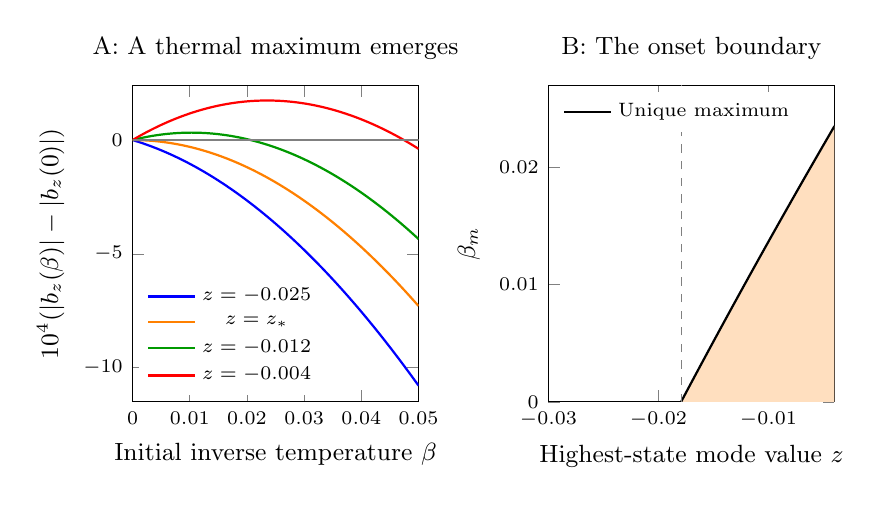
\begin{tikzpicture}
\begin{groupplot}[group style={group size=2 by 1,horizontal sep=1.65cm},width=.43\textwidth,height=5.6cm,tick label style={font=\scriptsize},label style={font=\small},title style={font=\small},scaled ticks=false]
\nextgroupplot[title={A: A thermal maximum emerges},xlabel={Initial inverse temperature $\beta$},ylabel={$10^4(|b_z(\beta)|-|b_z(0)|)$},xmin=0,xmax=.05,ymin=-11.5,ymax=2.4,xtick={0,.01,.02,.03,.04,.05},xticklabel style={/pgf/number format/fixed,/pgf/number format/precision=2},legend style={font=\scriptsize,draw=none,at={(.02,.02)},anchor=south west}]
\addplot[blue,thick] coordinates {(0.0,0.0) (0.0003333333333333334,-0.025435041859519596) (0.0006666666666666668,-0.05151647812271278) (0.001,-0.07824391076742812) (0.0013333333333333335,-0.10561694004242354) (0.001666666666666667,-0.1336351644729556) (0.002,-0.16229818086637288) (0.0023333333333333335,-0.1916055843177139) (0.002666666666666667,-0.22155696821530835) (0.0030000000000000005,-0.2521519242463828) (0.003333333333333334,-0.28339004240266985) (0.003666666666666667,-0.31527091098602145) (0.004,-0.34779411661402565) (0.004333333333333334,-0.3809592442256267) (0.004666666666666667,-0.41476587708674895) (0.005000000000000001,-0.44921359679592426) (0.005333333333333334,-0.4843019832899222) (0.005666666666666667,-0.5200306148493842) (0.006000000000000001,-0.5563990681044604) (0.006333333333333334,-0.5934069180404492) (0.006666666666666668,-0.6310537380034414) (0.007000000000000001,-0.6693390997059646) (0.007333333333333334,-0.7082625732326331) (0.007666666666666668,-0.7478237270457991) (0.008,-0.7880221279912062) (0.008333333333333335,-0.8288573413036473) (0.008666666666666668,-0.8703289306126223) (0.009000000000000001,-0.9124364579480008) (0.009333333333333334,-0.9551794837456857) (0.009666666666666667,-0.9985575668532796) (0.010000000000000002,-1.0425702645357526) (0.010333333333333335,-1.0872171324811126) (0.010666666666666668,-1.1324977248060788) (0.011000000000000001,-1.1784115940617548) (0.011333333333333334,-1.2249582912393056) (0.011666666666666669,-1.2721373657756354) (0.012000000000000002,-1.319948365559066) (0.012333333333333335,-1.3683908369350204) (0.012666666666666668,-1.4174643247117027) (0.013000000000000001,-1.467168372165785) (0.013333333333333336,-1.5175025210480912) (0.013666666666666669,-1.5684663115892832) (0.014000000000000002,-1.6200592825055509) (0.014333333333333335,-1.6722809710043003) (0.014666666666666668,-1.7251309127898433) (0.015000000000000001,-1.7786086420690892) (0.015333333333333336,-1.8327136915572373) (0.01566666666666667,-1.8874455924834679) (0.016,-1.9428038745966372) (0.016333333333333335,-1.9987880661709736) (0.01666666666666667,-2.0553976940117673) (0.017,-2.1126322834610693) (0.017333333333333336,-2.170491358403388) (0.017666666666666667,-2.2289744412713812) (0.018000000000000002,-2.2880810530515565) (0.018333333333333337,-2.3478107132899653) (0.018666666666666668,-2.4081629400978994) (0.019000000000000003,-2.469137250157591) (0.019333333333333334,-2.5307331587279034) (0.01966666666666667,-2.592950179650035) (0.020000000000000004,-2.6557878253532077) (0.020333333333333335,-2.7192456068603685) (0.02066666666666667,-2.783323033793885) (0.021,-2.848019614381236) (0.021333333333333336,-2.913334855460714) (0.02166666666666667,-2.9792682624871123) (0.022000000000000002,-3.045819339537421) (0.022333333333333337,-3.112987589316525) (0.02266666666666667,-3.180772513162886) (0.023000000000000003,-3.2491736110542444) (0.023333333333333338,-3.318190381613303) (0.02366666666666667,-3.387822322113419) (0.024000000000000004,-3.4580689284842916) (0.024333333333333335,-3.5289296953176494) (0.02466666666666667,-3.6004041158729385) (0.025000000000000005,-3.672491682083003) (0.025333333333333336,-3.7451918845597714) (0.02566666666666667,-3.8185042125999398) (0.026000000000000002,-3.892428154190649) (0.026333333333333337,-3.9669631960151657) (0.026666666666666672,-4.04210882345856) (0.027000000000000003,-4.117864520613377) (0.027333333333333338,-4.19422977028532) (0.02766666666666667,-4.271204053998911) (0.028000000000000004,-4.348786852003169) (0.028333333333333335,-4.426977643277275) (0.02866666666666667,-4.50577590553624) (0.029000000000000005,-4.585181115236564) (0.029333333333333336,-4.665192747581904) (0.02966666666666667,-4.745810276528732) (0.030000000000000002,-4.827033174791989) (0.030333333333333337,-4.908860913850743) (0.030666666666666672,-4.991292963953842) (0.031000000000000003,-5.074328794125557) (0.03133333333333334,-5.157967872171242) (0.03166666666666667,-5.242209664682966) (0.032,-5.3270536370451635) (0.03233333333333334,-5.412499253440272) (0.03266666666666667,-5.498545976854358) (0.033,-5.585193269082771) (0.03333333333333334,-5.672440590735756) (0.03366666666666667,-5.760287401244085) (0.034,-5.848733158864689) (0.03433333333333334,-5.937777320686274) (0.03466666666666667,-6.027419342634929) (0.035,-6.117658679479761) (0.035333333333333335,-6.208494784838493) (0.03566666666666667,-6.299927111183069) (0.036000000000000004,-6.391955109845269) (0.036333333333333336,-6.484578231022302) (0.036666666666666674,-6.577795923782408) (0.037000000000000005,-6.671607636070443) (0.037333333333333336,-6.766012814713482) (0.037666666666666675,-6.861010905426398) (0.038000000000000006,-6.956601352817437) (0.03833333333333334,-7.052783600393809) (0.03866666666666667,-7.149557090567256) (0.03900000000000001,-7.246921264659624) (0.03933333333333334,-7.344875562908423) (0.03966666666666667,-7.443419424472399) (0.04000000000000001,-7.542552287437087) (0.04033333333333334,-7.642273588820358) (0.04066666666666667,-7.742582764577981) (0.04100000000000001,-7.843479249609162) (0.04133333333333334,-7.9449624777620755) (0.04166666666666667,-8.047031881839414) (0.042,-8.149686893603917) (0.04233333333333334,-8.25292694378389) (0.04266666666666667,-8.356751462078726) (0.043000000000000003,-8.461159877164437) (0.04333333333333334,-8.566151616699152) (0.04366666666666667,-8.671726107328627) (0.044000000000000004,-8.777882774691754) (0.044333333333333336,-8.884621043426055) (0.044666666666666674,-8.991940337173174) (0.045000000000000005,-9.09984007858436) (0.04533333333333334,-9.208319689325965) (0.045666666666666675,-9.3173785900849) (0.046000000000000006,-9.427016200574124) (0.04633333333333334,-9.537231939538104) (0.046666666666666676,-9.64802522475828) (0.04700000000000001,-9.759395473058513) (0.04733333333333334,-9.87134210031054) (0.04766666666666667,-9.983864521439427) (0.04800000000000001,-10.096962150429) (0.04833333333333334,-10.210634400327274) (0.04866666666666667,-10.324880683251893) (0.04900000000000001,-10.43970041039555) (0.04933333333333334,-10.555092992031392) (0.04966666666666667,-10.671057837518447) (0.05,-10.78759435530702)};\addlegendentry{$z=-0.025$}
\addplot[orange,thick] coordinates {(0.0,0.0) (0.0003333333333333334,-0.0003351101266055592) (0.0006666666666666668,-0.0013401840059951292) (0.001,-0.003014835507794835) (0.0013333333333333335,-0.005358676666552211) (0.001666666666666667,-0.00837131768744747) (0.002,-0.012052366952009714) (0.0023333333333333335,-0.016401431023837988) (0.002666666666666667,-0.021418114654327046) (0.0030000000000000005,-0.02710202078839781) (0.003333333333333334,-0.033452750570232385) (0.003666666666666667,-0.04046990334901354) (0.004,-0.048153076684668644) (0.004333333333333334,-0.056501866353617806) (0.004666666666666667,-0.06551586635452623) (0.005000000000000001,-0.07519466891406093) (0.005333333333333334,-0.08553786449265101) (0.005666666666666667,-0.09654504179025249) (0.006000000000000001,-0.10821578775211649) (0.006333333333333334,-0.12054968757456137) (0.006666666666666668,-0.13354632471074876) (0.007000000000000001,-0.14720528087646273) (0.007333333333333334,-0.16152613605589305) (0.007666666666666668,-0.17650846850742138) (0.008,-0.1921518547694109) (0.008333333333333335,-0.20845586966599983) (0.008666666666666668,-0.22542008631289662) (0.009000000000000001,-0.2430440761231802) (0.009333333333333334,-0.2613274088131016) (0.009666666666666667,-0.28026965240788926) (0.010000000000000002,-0.29987037324755716) (0.010333333333333335,-0.320129135992715) (0.010666666666666668,-0.34104550363038216) (0.011000000000000001,-0.3626190374798035) (0.011333333333333334,-0.38484929719826766) (0.011666666666666669,-0.40773584078692793) (0.012000000000000002,-0.43127822459662524) (0.012333333333333335,-0.4554760033337139) (0.012666666666666668,-0.48032873006588894) (0.013000000000000001,-0.5058359562280158) (0.013333333333333336,-0.531997231627962) (0.013666666666666669,-0.5588121044524299) (0.014000000000000002,-0.5862801212727934) (0.014333333333333335,-0.6144008270509337) (0.014666666666666668,-0.6431737651450788) (0.015000000000000001,-0.6725984773156436) (0.015333333333333336,-0.7026745037310715) (0.01566666666666667,-0.7334013829736777) (0.016,-0.7647786520454934) (0.016333333333333335,-0.7968058463741131) (0.01666666666666667,-0.829482499818539) (0.017,-0.8628081446750305) (0.017333333333333336,-0.8967823116829545) (0.017666666666666667,-0.9314045300306321) (0.018000000000000002,-0.9666743273611929) (0.018333333333333337,-1.0025912297784236) (0.018666666666666668,-1.039154761852622) (0.019000000000000003,-1.0763644466264506) (0.019333333333333334,-1.114219805620787) (0.01966666666666667,-1.1527203588405814) (0.020000000000000004,-1.1918656247807076) (0.020333333333333335,-1.2316551204318194) (0.02066666666666667,-1.2720883612862057) (0.021,-1.3131648613436429) (0.021333333333333336,-1.3548841331172536) (0.02166666666666667,-1.3972456876393575) (0.022000000000000002,-1.4402490344673287) (0.022333333333333337,-1.4838936816894504) (0.02266666666666667,-1.5281791359307677) (0.023000000000000003,-1.5731049023589432) (0.023333333333333338,-1.6186704846901103) (0.02366666666666667,-1.664875385194725) (0.024000000000000004,-1.7117191047034215) (0.024333333333333335,-1.7592011426128606) (0.02466666666666667,-1.807320996891585) (0.025000000000000005,-1.8560781640858661) (0.025333333333333336,-1.9054721393255554) (0.02566666666666667,-1.9555024163299342) (0.026000000000000002,-2.0061684874135595) (0.026333333333333337,-2.0574698434921124) (0.026666666666666672,-2.1094059740882423) (0.027000000000000003,-2.161976367337411) (0.027333333333333338,-2.215180509993738) (0.02766666666666667,-2.2690178874358398) (0.028000000000000004,-2.3234879836726714) (0.028333333333333335,-2.378590281349364) (0.02866666666666667,-2.434324261753064) (0.029000000000000005,-2.4906894048187658) (0.029333333333333336,-2.5476851891351475) (0.02966666666666667,-2.605311091950404) (0.030000000000000002,-2.663566589178073) (0.030333333333333337,-2.7224511554028674) (0.030666666666666672,-2.781964263886499) (0.031000000000000003,-2.842105386573503) (0.03133333333333334,-2.902873994097063) (0.03166666666666667,-2.964269555784822) (0.032,-3.026291539664712) (0.03233333333333334,-3.0889394124707614) (0.03266666666666667,-3.152212639648905) (0.033,-3.216110685362803) (0.03333333333333334,-3.2806330124996435) (0.03366666666666667,-3.3457790826759424) (0.034,-3.4115483562433577) (0.03433333333333334,-3.4779402922944813) (0.03466666666666667,-3.5449543486686306) (0.035,-3.612589981957655) (0.035333333333333335,-3.6808466475117187) (0.03566666666666667,-3.7497237994450883) (0.036000000000000004,-3.8192208906419185) (0.036333333333333336,-3.8893373727620353) (0.036666666666666674,-3.9600726962467148) (0.037000000000000005,-4.031426310324451) (0.037333333333333336,-4.103397663016738) (0.037666666666666675,-4.175986201143833) (0.038000000000000006,-4.249191370330516) (0.03833333333333334,-4.323012615011861) (0.03866666666666667,-4.397449378438986) (0.03900000000000001,-4.472501102684812) (0.03933333333333334,-4.548167228649805) (0.03966666666666667,-4.624447196067733) (0.04000000000000001,-4.701340443511402) (0.04033333333333334,-4.778846408398393) (0.04066666666666667,-4.856964526996801) (0.04100000000000001,-4.935694234430968) (0.04133333333333334,-5.015034964687193) (0.04166666666666667,-5.094986150619479) (0.042,-5.175547223955231) (0.04233333333333334,-5.25671761530098) (0.04266666666666667,-5.338496754148082) (0.043000000000000003,-5.420884068878438) (0.04333333333333334,-5.503878986770181) (0.04366666666666667,-5.587480934003378) (0.044000000000000004,-5.671689335665719) (0.044333333333333336,-5.756503615758206) (0.044666666666666674,-5.841923197200833) (0.045000000000000005,-5.9279475018382595) (0.04533333333333334,-6.014575950445493) (0.045666666666666675,-6.1018079627335435) (0.046000000000000006,-6.189642957355094) (0.04633333333333334,-6.278080351910158) (0.046666666666666676,-6.3671195629517285) (0.04700000000000001,-6.456760005991424) (0.04733333333333334,-6.547001095505134) (0.04766666666666667,-6.637842244938655) (0.04800000000000001,-6.729282866713325) (0.04833333333333334,-6.821322372231635) (0.04866666666666667,-6.913960171882871) (0.04900000000000001,-7.007195675048718) (0.04933333333333334,-7.101028290108862) (0.04966666666666667,-7.1954574244466105) (0.05,-7.290482484454481)};\addlegendentry{$z=z_*$}
\addplot[green!60!black,thick] coordinates {(0.0,0.0) (0.0003333333333333334,0.0207836908785624) (0.0006666666666666668,0.04087758701838509) (0.001,0.0602820645442337) (0.0013333333333333335,0.07899750150512955) (0.001666666666666667,0.09702427786853562) (0.002,0.11436277551453723) (0.0023333333333333335,0.1310133782300171) (0.002666666666666667,0.14697647170282502) (0.0030000000000000005,0.16225244351594229) (0.003333333333333334,0.17684168314164095) (0.003666666666666667,0.19074458193563798) (0.004,0.2039615331312444) (0.004333333333333334,0.2164929318335096) (0.004666666666666667,0.22833917501336043) (0.005000000000000001,0.23950066150173632) (0.005333333333333334,0.249977791983719) (0.005666666666666667,0.2597709689926581) (0.006000000000000001,0.2688805969042922) (0.006333333333333334,0.27730708193086545) (0.006666666666666668,0.28505083211523996) (0.007000000000000001,0.29211225732500395) (0.007333333333333334,0.29849176924657594) (0.007666666666666668,0.30418978137930497) (0.008,0.3092067090295664) (0.008333333333333335,0.3135429693048545) (0.008666666666666668,0.3171989811078712) (0.009000000000000001,0.32017516513061073) (0.009333333333333334,0.3224719438484412) (0.009666666666666667,0.3240897415141825) (0.010000000000000002,0.32502898415218084) (0.010333333333333335,0.3252900995523799) (0.010666666666666668,0.32487351726438907) (0.011000000000000001,0.323779668591548) (0.011333333333333334,0.32200898658498883) (0.011666666666666669,0.31956190603769496) (0.012000000000000002,0.31643886347855704) (0.012333333333333335,0.31264029716642655) (0.012666666666666668,0.3081666470841659) (0.013000000000000001,0.303018354932697) (0.013333333333333336,0.29719586412504634) (0.013666666666666669,0.2906996197803882) (0.014000000000000002,0.28353006871808545) (0.014333333333333335,0.27568765945172785) (0.014666666666666668,0.26717284218316845) (0.015000000000000001,0.25798606879655767) (0.015333333333333336,0.24812779285237563) (0.01566666666666667,0.2375984695814625) (0.016,0.22639855587904686) (0.016333333333333335,0.21452851029877193) (0.01666666666666667,0.2019887930467216) (0.017,0.18877986597544327) (0.017333333333333336,0.17490219257796935) (0.017666666666666667,0.16035623798183912) (0.018000000000000002,0.14514246894311636) (0.018333333333333337,0.1292613538404086) (0.018666666666666668,0.1127133626688835) (0.019000000000000003,0.0954989670342838) (0.019333333333333334,0.07761864014694356) (0.01966666666666667,0.05907285681580013) (0.020000000000000004,0.039862093442408944) (0.020333333333333335,0.019986828014954494) (0.02066666666666667,-0.000552459897738349) (0.021,-0.02175528915219192) (0.021333333333333336,-0.04362117703626762) (0.02166666666666667,-0.06614963927515345) (0.022000000000000002,-0.08934019003735615) (0.022333333333333337,-0.1131923419406917) (0.02266666666666667,-0.1377056060582751) (0.023000000000000003,-0.1628794919245126) (0.023333333333333338,-0.18871350754109212) (0.02366666666666667,-0.21520715938297383) (0.024000000000000004,-0.24235995240438218) (0.024333333333333335,-0.270171390044795) (0.02466666666666667,-0.2986409742349358) (0.025000000000000005,-0.3277682054027616) (0.025333333333333336,-0.35755258247945365) (0.02566666666666667,-0.3879936029054075) (0.026000000000000002,-0.4190907626362194) (0.026333333333333337,-0.45084355614867594) (0.026666666666666672,-0.4832514764467398) (0.027000000000000003,-0.5163140150675365) (0.027333333333333338,-0.5500306620873409) (0.02766666666666667,-0.5844009061275592) (0.028000000000000004,-0.619424234360715) (0.028333333333333335,-0.6551001325164292) (0.02866666666666667,-0.6914280848874033) (0.029000000000000005,-0.7284075743353968) (0.029333333333333336,-0.7660380822972072) (0.02966666666666667,-0.8043190887906472) (0.030000000000000002,-0.8432500724205192) (0.030333333333333337,-0.8828305103845904) (0.030666666666666672,-0.9230598784795636) (0.031000000000000003,-0.963937651107049) (0.03133333333333334,-1.0054633012795342) (0.03166666666666667,-1.047636300626347) (0.032,-1.0904561193996256) (0.03233333333333334,-1.1339222264802802) (0.03266666666666667,-1.1780340893839485) (0.033,-1.2227911742669635) (0.03333333333333334,-1.2681929459323058) (0.03366666666666667,-1.3142388678355534) (0.034,-1.3609284020908425) (0.03433333333333334,-1.408261009476813) (0.03466666666666667,-1.4562361494425509) (0.035,-1.504853280113541) (0.035333333333333335,-1.5541118582976046) (0.03566666666666667,-1.6040113394908375) (0.036000000000000004,-1.6545511778835482) (0.036333333333333336,-1.7057308263661912) (0.036666666666666674,-1.757549736535299) (0.037000000000000005,-1.8100073586994048) (0.037333333333333336,-1.8631031418849733) (0.037666666666666675,-1.9168365338423203) (0.038000000000000006,-1.9712069810515254) (0.03833333333333334,-2.0262139287283567) (0.03866666666666667,-2.0818568208301738) (0.03900000000000001,-2.1381351000618443) (0.03933333333333334,-2.195048207881638) (0.03966666666666667,-2.2525955845071395) (0.04000000000000001,-2.310776668921141) (0.04033333333333334,-2.3695908988775307) (0.04066666666666667,-2.4290377109071963) (0.04100000000000001,-2.4891165403239017) (0.04133333333333334,-2.549826821230169) (0.04166666666666667,-2.611167986523165) (0.042,-2.6731394679005707) (0.04233333333333334,-2.735740695866455) (0.04266666666666667,-2.7989710997371344) (0.043000000000000003,-2.8628301076470484) (0.04333333333333334,-2.9273171465546075) (0.04366666666666667,-2.992431642248048) (0.044000000000000004,-3.058173019351289) (0.044333333333333336,-3.124540701329771) (0.044666666666666674,-3.191534110496299) (0.045000000000000005,-3.2591526680168776) (0.04533333333333334,-3.3273957939165473) (0.045666666666666675,-3.396262907085205) (0.046000000000000006,-3.465753425283431) (0.04633333333333334,-3.5358667651483064) (0.046666666666666676,-3.6066023421992246) (0.04700000000000001,-3.677959570843697) (0.04733333333333334,-3.7499378643831616) (0.04766666666666667,-3.822536635018776) (0.04800000000000001,-3.895755293857216) (0.04833333333333334,-3.9695932509164518) (0.04866666666666667,-4.044049915131544) (0.04900000000000001,-4.1191246943604165) (0.04933333333333334,-4.19481699538962) (0.04966666666666667,-4.2711262239401115) (0.05,-4.348051784673009)};\addlegendentry{$z=-0.012$}
\addplot[red,thick] coordinates {(0.0,0.0) (0.0003333333333333334,0.04922598794815132) (0.0006666666666666668,0.0977354732590607) (0.001,0.14552881858217945) (0.0013333333333333335,0.19260638861131607) (0.001666666666666667,0.23896855007868406) (0.002,0.2846156717489434) (0.0023333333333333335,0.3295481244132362) (0.002666666666666667,0.3737662808832148) (0.0030000000000000005,0.41727051598506537) (0.003333333333333334,0.4600612065535245) (0.003666666666666667,0.5021387314258899) (0.004,0.543503471436026) (0.004333333333333334,0.5841558094083626) (0.004666666666666667,0.6240961301518893) (0.005000000000000001,0.6633248204541429) (0.005333333333333334,0.7018422690751905) (0.005666666666666667,0.7396488667416072) (0.006000000000000001,0.7767450061404477) (0.006333333333333334,0.8131310819132129) (0.006666666666666668,0.8488074906498131) (0.007000000000000001,0.8837746308825231) (0.007333333333333334,0.9180329030799355) (0.007666666666666668,0.9515827096409075) (0.008,0.9844244548885033) (0.008333333333333335,1.0165585450639325) (0.008666666666666668,1.0479853883204826) (0.009000000000000001,1.0787053947174485) (0.009333333333333334,1.1087189762140577) (0.009666666666666667,1.1380265466633899) (0.010000000000000002,1.1666285218062937) (0.010333333333333335,1.1945253192652985) (0.010666666666666668,1.221717358538523) (0.011000000000000001,1.2482050609935804) (0.011333333333333334,1.2739888498614778) (0.011666666666666669,1.2990691502305136) (0.012000000000000002,1.3234463890401713) (0.012333333333333335,1.3471209950750092) (0.012666666666666668,1.3700933989585466) (0.013000000000000001,1.3923640331471476) (0.013333333333333336,1.4139333319239002) (0.013666666666666669,1.4348017313924937) (0.014000000000000002,1.4549696694710925) (0.014333333333333335,1.4744375858862067) (0.014666666666666668,1.4932059221665603) (0.015000000000000001,1.5112751216369558) (0.015333333333333336,1.5286456294121373) (0.01566666666666667,1.5453178923906505) (0.016,1.5612923592486987) (0.016333333333333335,1.576569480434) (0.01666666666666667,1.591149708159638) (0.017,1.6050334963979125) (0.017333333333333336,1.6182213008741893) (0.017666666666666667,1.6307135790607439) (0.018000000000000002,1.6425107901706073) (0.018333333333333337,1.6536133951514078) (0.018666666666666668,1.6640218566792113) (0.019000000000000003,1.6737366391523605) (0.019333333333333334,1.682758208685311) (0.01966666666666667,1.6910870331024679) (0.020000000000000004,1.6987235819320192) (0.020333333333333335,1.7056683263997687) (0.02066666666666667,1.711921739422967) (0.021,1.7174842956041427) (0.021333333333333336,1.7223564712249302) (0.02166666666666667,1.726538744239898) (0.022000000000000002,1.7300315942703763) (0.022333333333333337,1.7328355025982825) (0.02266666666666667,1.734950952159947) (0.023000000000000003,1.7363784275399379) (0.023333333333333338,1.737118414964884) (0.02366666666666667,1.7371714022973) (0.024000000000000004,1.7365378790294081) (0.024333333333333335,1.7352183362769615) (0.02466666666666667,1.7332132667730658) (0.025000000000000005,1.7305231648620023) (0.025333333333333336,1.7271485264930495) (0.02566666666666667,1.7230898492143047) (0.026000000000000002,1.7183476321665063) (0.026333333333333337,1.7129223760768564) (0.026666666666666672,1.7068145832528416) (0.027000000000000003,1.7000247575760579) (0.027333333333333338,1.6925534044960309) (0.02766666666666667,1.6844010310240418) (0.028000000000000004,1.6755681457269491) (0.028333333333333335,1.6660552587210145) (0.02866666666666667,1.6558628816657268) (0.029000000000000005,1.644991527757629) (0.029333333333333336,1.6334417117241449) (0.02966666666666667,1.6212139498174052) (0.030000000000000002,1.6083087598080776) (0.030333333333333337,1.5947266609791961) (0.030666666666666672,1.580468174119992) (0.031000000000000003,1.565533821519725) (0.03133333333333334,1.5499241269615172) (0.03166666666666667,1.533639615716188) (0.032,1.5166808145360902) (0.03233333333333334,1.4990482516489456) (0.03266666666666667,1.4807424567516885) (0.033,1.4617639610043023) (0.03333333333333334,1.4421132970236636) (0.03366666666666667,1.4217909988773894) (0.034,1.4007976020776782) (0.03433333333333334,1.3791336435751624) (0.03466666666666667,1.3567996617527587) (0.035,1.3337961964195177) (0.035333333333333335,1.3101237888044803) (0.03566666666666667,1.2857829815505362) (0.036000000000000004,1.2607743187082803) (0.036333333333333336,1.235098345729877) (0.036666666666666674,1.2087556094629217) (0.037000000000000005,1.181746658144311) (0.037333333333333336,1.154072041394109) (0.037666666666666675,1.12573231020942) (0.038000000000000006,1.096728016958266) (0.03833333333333334,1.0670597153734604) (0.03866666666666667,1.036727960546492) (0.03900000000000001,1.0057333089214051) (0.03933333333333334,0.9740763182886915) (0.03966666666666667,0.9417575477791742) (0.04000000000000001,0.9087775578579034) (0.04033333333333334,0.875136910318055) (0.04066666666666667,0.840836168274825) (0.04100000000000001,0.8058758961593352) (0.04133333333333334,0.7702566597125425) (0.04166666666666667,0.7339790259791429) (0.042,0.6970435633014891) (0.04233333333333334,0.6594508413135057) (0.04266666666666667,0.6212014309346146) (0.043000000000000003,0.5822959043636524) (0.04333333333333334,0.5427348350728051) (0.04366666666666667,0.5025187978015393) (0.044000000000000004,0.46164836855053604) (0.044333333333333336,0.4201241245756356) (0.044666666666666674,0.37794664438177833) (0.045000000000000005,0.33511650771695844) (0.04533333333333334,0.2916342955661715) (0.045666666666666675,0.24750059014537665) (0.046000000000000006,0.2027159748954571) (0.04633333333333334,0.15728103447618494) (0.046666666666666676,0.11119635476019464) (0.04700000000000001,0.06446252282695795) (0.04733333333333334,0.017080126956763506) (0.04766666666666667,-0.03095024337529894) (0.04800000000000001,-0.07962799750534882) (0.04833333333333334,-0.12895254358671496) (0.04866666666666667,-0.1789232885959449) (0.04900000000000001,-0.22953963833879618) (0.04933333333333334,-0.2808009974562224) (0.04966666666666667,-0.33270676943036775) (0.05,-0.3852563565905413)};\addlegendentry{$z=-0.004$}
\addplot[gray,forget plot] coordinates {(0,0)(.05,0)};
\nextgroupplot[title={B: The onset boundary},xlabel={Highest-state mode value $z$},ylabel={$\beta_m$},xmin=-.03,xmax=-.004,ymin=0,ymax=.027,xtick={-.03,-.02,-.01},ytick={0,.01,.02},xticklabel style={/pgf/number format/fixed,/pgf/number format/precision=2},yticklabel style={/pgf/number format/fixed,/pgf/number format/precision=2},legend style={font=\scriptsize,draw=none,at={(.02,.98)},anchor=north west}]
\addplot[fill=orange!25,draw=none,forget plot] coordinates {(-0.017940111223364898,0.0) (-0.017800710111131247,0.0002464413443806452) (-0.0176613089988976,0.0004926451841585077) (-0.01752190788666395,0.0007386118890034555) (-0.0173825067744303,0.0009843418279155665) (-0.017243105662196653,0.0012298353692260999) (-0.017103704549963003,0.0014750928805984682) (-0.016964303437729356,0.0017201147290291602) (-0.016824902325495706,0.001964901280848743) (-0.016685501213262056,0.0022094529017227865) (-0.01654610010102841,0.0024537699566528426) (-0.01640669898879476,0.002697852809977433) (-0.01626729787656111,0.002941701825372973) (-0.01612789676432746,0.003185317365854769) (-0.01598849565209381,0.0034286997937779803) (-0.015849094539860165,0.0036718494708385843) (-0.015709693427626514,0.003914766758074382) (-0.015570292315392864,0.004157452015865918) (-0.015430891203159216,0.004399905603937492) (-0.015291490090925567,0.004642127881358138) (-0.015152088978691918,0.004884119206542585) (-0.01501268786645827,0.005125879937252245) (-0.01487328675422462,0.005367410430596202) (-0.014733885641990971,0.005608711043032173) (-0.014594484529757323,0.005849782130367511) (-0.014455083417523672,0.006090624047760189) (-0.014315682305290024,0.0063312371497197635) (-0.014176281193056375,0.006571621790108394) (-0.014036880080822725,0.006811778322141807) (-0.013897478968589078,0.0070517070983902854) (-0.013758077856355428,0.0072914084707796836) (-0.01361867674412178,0.0075308827905923815) (-0.013479275631888131,0.007770130408468309) (-0.01333987451965448,0.008009151674405923) (-0.013200473407420832,0.00824794693776319) (-0.013061072295187184,0.00848651654725862) (-0.012921671182953533,0.008724860850972226) (-0.012782270070719885,0.008962980196346523) (-0.012642868958486236,0.009200874930187551) (-0.012503467846252586,0.009438545398665852) (-0.01236406673401894,0.009675991947317462) (-0.012224665621785289,0.009913214921044956) (-0.01208526450955164,0.01015021466411838) (-0.011945863397317992,0.010386991520176308) (-0.011806462285084342,0.010623545832226832) (-0.011667061172850693,0.010859877942648541) (-0.011527660060617045,0.011095988193191552) (-0.011388258948383394,0.01133187692497851) (-0.011248857836149746,0.01156754447850557) (-0.011109456723916097,0.011802991193643432) (-0.010970055611682447,0.012038217409638334) (-0.0108306544994488,0.012273223465113052) (-0.01069125338721515,0.012508009698067925) (-0.010551852274981502,0.01274257644588184) (-0.010412451162747853,0.012976924045313261) (-0.010273050050514203,0.013211052832501223) (-0.010133648938280554,0.013444963142966346) (-0.009994247826046906,0.013678655311611845) (-0.009854846713813257,0.013912129672724543) (-0.009715445601579607,0.014145386559975878) (-0.009576044489345958,0.014378426306422904) (-0.00943664337711231,0.01461124924450932) (-0.009297242264878661,0.01484385570606647) (-0.009157841152645011,0.015076246022314358) (-0.009018440040411363,0.015308420523862653) (-0.008879038928177714,0.015540379540711713) (-0.008739637815944064,0.015772123402253587) (-0.008600236703710415,0.016003652437273034) (-0.008460835591476767,0.016234966973948526) (-0.008321434479243118,0.01646606733985328) (-0.008182033367009468,0.016696953861956246) (-0.00804263225477582,0.016927626866623142) (-0.007903231142542171,0.01715808667961746) (-0.007763830030308522,0.017388333626101468) (-0.007624428918074872,0.01761836803063724) (-0.007485027805841224,0.017848190217187664) (-0.007345626693607575,0.018077800509117448) (-0.0072062255813739266,0.018307199229194153) (-0.007066824469140276,0.01853638669958918) (-0.006927423356906628,0.018765363241878802) (-0.006788022244672979,0.018994129177045183) (-0.006648621132439329,0.01922268482547737) (-0.0065092200202056805,0.01945103050697232) (-0.006369818907972032,0.01967916654073592) (-0.006230417795738383,0.019907093245383988) (-0.006091016683504733,0.020134810938943294) (-0.005951615571271085,0.02036231993885256) (-0.005812214459037436,0.0205896205619635) (-0.005672813346803788,0.0208167131245418) (-0.005533412234570137,0.021043597942268167) (-0.005394011122336489,0.021270275330239303) (-0.00525461001010284,0.021496745602968947) (-0.005115208897869192,0.021723009074388868) (-0.0049758077856355415,0.021949066057849905) (-0.004836406673401893,0.02217491686612294) (-0.0046970055611682444,0.022400561811399933) (-0.004557604448934594,0.022626001205294937) (-0.004418203336700946,0.022851235358845094) (-0.004278802224467297,0.02307626458251166) (-0.004139401112233649,0.023301089186181005) (-0.004,0.023525709479165623) (-.004,0)} --cycle;
\addplot[black,thick] coordinates {(-0.017940111223364898,0.0) (-0.017800710111131247,0.0002464413443806452) (-0.0176613089988976,0.0004926451841585077) (-0.01752190788666395,0.0007386118890034555) (-0.0173825067744303,0.0009843418279155665) (-0.017243105662196653,0.0012298353692260999) (-0.017103704549963003,0.0014750928805984682) (-0.016964303437729356,0.0017201147290291602) (-0.016824902325495706,0.001964901280848743) (-0.016685501213262056,0.0022094529017227865) (-0.01654610010102841,0.0024537699566528426) (-0.01640669898879476,0.002697852809977433) (-0.01626729787656111,0.002941701825372973) (-0.01612789676432746,0.003185317365854769) (-0.01598849565209381,0.0034286997937779803) (-0.015849094539860165,0.0036718494708385843) (-0.015709693427626514,0.003914766758074382) (-0.015570292315392864,0.004157452015865918) (-0.015430891203159216,0.004399905603937492) (-0.015291490090925567,0.004642127881358138) (-0.015152088978691918,0.004884119206542585) (-0.01501268786645827,0.005125879937252245) (-0.01487328675422462,0.005367410430596202) (-0.014733885641990971,0.005608711043032173) (-0.014594484529757323,0.005849782130367511) (-0.014455083417523672,0.006090624047760189) (-0.014315682305290024,0.0063312371497197635) (-0.014176281193056375,0.006571621790108394) (-0.014036880080822725,0.006811778322141807) (-0.013897478968589078,0.0070517070983902854) (-0.013758077856355428,0.0072914084707796836) (-0.01361867674412178,0.0075308827905923815) (-0.013479275631888131,0.007770130408468309) (-0.01333987451965448,0.008009151674405923) (-0.013200473407420832,0.00824794693776319) (-0.013061072295187184,0.00848651654725862) (-0.012921671182953533,0.008724860850972226) (-0.012782270070719885,0.008962980196346523) (-0.012642868958486236,0.009200874930187551) (-0.012503467846252586,0.009438545398665852) (-0.01236406673401894,0.009675991947317462) (-0.012224665621785289,0.009913214921044956) (-0.01208526450955164,0.01015021466411838) (-0.011945863397317992,0.010386991520176308) (-0.011806462285084342,0.010623545832226832) (-0.011667061172850693,0.010859877942648541) (-0.011527660060617045,0.011095988193191552) (-0.011388258948383394,0.01133187692497851) (-0.011248857836149746,0.01156754447850557) (-0.011109456723916097,0.011802991193643432) (-0.010970055611682447,0.012038217409638334) (-0.0108306544994488,0.012273223465113052) (-0.01069125338721515,0.012508009698067925) (-0.010551852274981502,0.01274257644588184) (-0.010412451162747853,0.012976924045313261) (-0.010273050050514203,0.013211052832501223) (-0.010133648938280554,0.013444963142966346) (-0.009994247826046906,0.013678655311611845) (-0.009854846713813257,0.013912129672724543) (-0.009715445601579607,0.014145386559975878) (-0.009576044489345958,0.014378426306422904) (-0.00943664337711231,0.01461124924450932) (-0.009297242264878661,0.01484385570606647) (-0.009157841152645011,0.015076246022314358) (-0.009018440040411363,0.015308420523862653) (-0.008879038928177714,0.015540379540711713) (-0.008739637815944064,0.015772123402253587) (-0.008600236703710415,0.016003652437273034) (-0.008460835591476767,0.016234966973948526) (-0.008321434479243118,0.01646606733985328) (-0.008182033367009468,0.016696953861956246) (-0.00804263225477582,0.016927626866623142) (-0.007903231142542171,0.01715808667961746) (-0.007763830030308522,0.017388333626101468) (-0.007624428918074872,0.01761836803063724) (-0.007485027805841224,0.017848190217187664) (-0.007345626693607575,0.018077800509117448) (-0.0072062255813739266,0.018307199229194153) (-0.007066824469140276,0.01853638669958918) (-0.006927423356906628,0.018765363241878802) (-0.006788022244672979,0.018994129177045183) (-0.006648621132439329,0.01922268482547737) (-0.0065092200202056805,0.01945103050697232) (-0.006369818907972032,0.01967916654073592) (-0.006230417795738383,0.019907093245383988) (-0.006091016683504733,0.020134810938943294) (-0.005951615571271085,0.02036231993885256) (-0.005812214459037436,0.0205896205619635) (-0.005672813346803788,0.0208167131245418) (-0.005533412234570137,0.021043597942268167) (-0.005394011122336489,0.021270275330239303) (-0.00525461001010284,0.021496745602968947) (-0.005115208897869192,0.021723009074388868) (-0.0049758077856355415,0.021949066057849905) (-0.004836406673401893,0.02217491686612294) (-0.0046970055611682444,0.022400561811399933) (-0.004557604448934594,0.022626001205294937) (-0.004418203336700946,0.022851235358845094) (-0.004278802224467297,0.02307626458251166) (-0.004139401112233649,0.023301089186181005) (-0.004,0.023525709479165623)};\addlegendentry{Unique maximum}
\addplot[gray,dashed,forget plot] coordinates {(-.0179401112234,0)(-.0179401112234,.027)};
\end{groupplot}
\end{tikzpicture}
\caption{Predictive family of Theorem~\ref{thm:family}. All four triplet predicates fail throughout. Above $z_*$ the amplitude initially increases with inverse temperature and has exactly one cooling maximum; below $z_*$ it decreases throughout cooling. The shaded region has $\partial_\beta|b_z|>0$, so any two finite inverse temperatures inside one vertical slice give a witness. The $\beta=0$ limit is only a reference for the left ordinate. Curves are numerical; the onset and single-turn classification have a continuous-parameter proof.}
\label{fig:mechanism}
\end{figure}


This makes the neutral-state explanation predictive. Raising $z$ toward zero decreases the negative slow-mode weight carried by state 4, while its small bath weight requires only the weak adjustment $\eta z$ in state 3. The two rate formulas enforce that geometry, the spectral comparison makes it dynamically dominant, and $U-Vz<0$ quantifies when high-temperature occupation of state 4 reverses thermal ordering. The theorem classifies this controlled family and the stated single-turn geometry; it does not classify every four-state counterexample or every finite-time transient crossing. The covariance and spectral tools are established; no exhaustive priority claim is made for this particular construction or lemma.

\paragraph{Continuous-parameter verification.}
Run \path{research/mechanism_certificate.py}. It checks the rational eigenvector identities, all original triplet inequalities and the two branches on the entire interval. For each rational inequality, it clears the nonvanishing denominator, substitutes $z=-3/100+(13/500)t$, and verifies positive Bernstein coefficients on $0\leq t\leq1$. Since the Bernstein basis is nonnegative and sums to one, these are certificates over a continuum, not sampled evidence. The script records every coefficient and the baseline inertia pivots; a second spectral check bounds the remaining quadratic using its value at $-50$ and the mean of its two real roots.

Logarithms are reduced to arguments in $[1,2]$. With $x=(a-1)/(a+1)$, the positive series $2\sum_{k=0}^{m-1}x^{2k+1}/(2k+1)$ bounds $\log a$ from below, and its remainder is at most $2x^{2m+1}/[(2m+1)(1-x^2)]$. Rational bounds with $m=45$ certify the onset bracket and coefficient signs. Integer bisection bounds the algebraic Gibbs weights for the finite-pair threshold. Separately, \path{research/mechanism_plots.py} checks eight family members against symmetric diagonalization and numerical differentiation at 65-digit precision. Those checks and the plotted curves are illustrative cross-checks, not the continuous proof.


\subsection{Visible reversal and its size}
Figures~\ref{fig:overlap} and \ref{fig:crossing} separate two facts: the hotter initial state has a smaller slow-mode amplitude, and the full time-dependent distance actually changes ordering. These use the primary generator in Theorem~1, with the bath and generator fixed throughout. The high-temperature amplitude reaches its numerical maximum near $\beta=0.0237422$.

\begin{figure}[htbp]
\centering
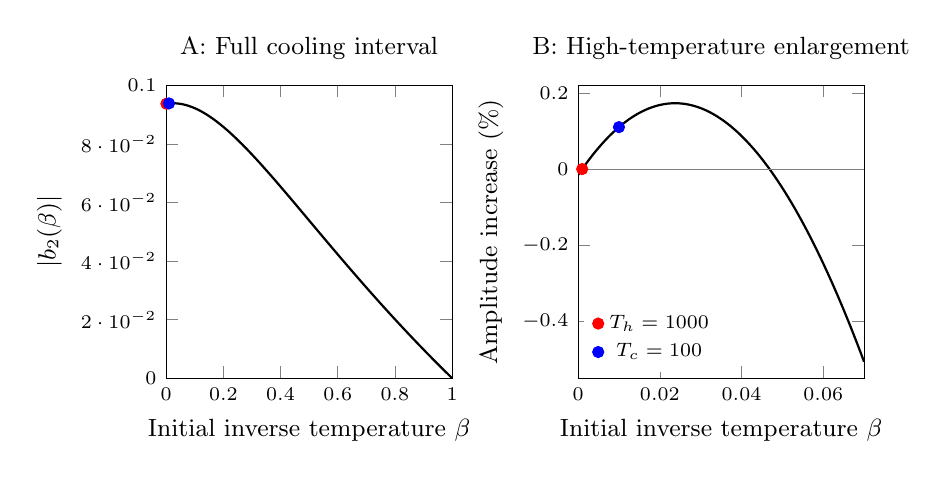
\begin{tikzpicture}
\begin{groupplot}[group style={group size=2 by 1,horizontal sep=1.6cm},width=0.43\textwidth,height=5.3cm,tick label style={font=\scriptsize},label style={font=\small},title style={font=\small},xlabel={Initial inverse temperature $\beta$},scaled ticks=false]
\nextgroupplot[title={A: Full cooling interval},xmin=0,xmax=1,ymin=0,ymax=.1,ylabel={$|b_2(\beta)|$}]
\addplot[black,thick] coordinates {(0,0.0937307280879) (0.008595988539,0.0938361114547) (0.01719197708,0.0938944479609) (0.02578796562,0.0939064820036) (0.03438395415,0.0938730351736) (0.04297994269,0.0937949992222) (0.05157593123,0.0936733290335) (0.06017191977,0.0935090356587) (0.06876790831,0.093303179468) (0.07736389685,0.0930568634644) (0.08595988539,0.0927712268026) (0.09455587393,0.0924474385483) (0.1031518625,0.0920866917064) (0.111747851,0.091690197544) (0.1203438395,0.0912591802263) (0.1289398281,0.0907948717793) (0.1375358166,0.0902985073893) (0.1461318052,0.0897713210442) (0.1547277937,0.0892145415173) (0.1633237822,0.0886293886924) (0.1719197708,0.088017070225) (0.1805157593,0.087378778531) (0.1891117479,0.0867156880944) (0.1977077364,0.0860289530815) (0.2063037249,0.085319705248) (0.2148997135,0.0845890521258) (0.223495702,0.0838380754735) (0.2320916905,0.0830678299749) (0.2406876791,0.0822793421697) (0.2492836676,0.0814736095994) (0.2578796562,0.0806516001538) (0.2664756447,0.0798142515995) (0.2750716332,0.0789624712781) (0.2836676218,0.0780971359555) (0.2922636103,0.0772190918105) (0.3008595989,0.0763291545473) (0.3094555874,0.0754281096185) (0.3180515759,0.0745167125467) (0.3266475645,0.0735956893329) (0.335243553,0.0726657369393) (0.3438395415,0.0717275238384) (0.3524355301,0.0707816906165) (0.3610315186,0.0698288506244) (0.3696275072,0.0688695906667) (0.3782234957,0.0679044717215) (0.3868194842,0.0669340296855) (0.3954154728,0.0659587761365) (0.4040114613,0.0649791991088) (0.4126074499,0.0639957638763) (0.4212034384,0.0630089137392) (0.4297994269,0.0620190708094) (0.4383954155,0.0610266367929) (0.446991404,0.0600319937636) (0.4555873926,0.0590355049289) (0.4641833811,0.058037515382) (0.4727793696,0.057038352841) (0.4813753582,0.0560383283716) (0.4899713467,0.0550377370939) (0.4985673352,0.0540368588702) (0.5071633238,0.0530359589736) (0.5157593123,0.0520352887381) (0.5243553009,0.0510350861871) (0.5329512894,0.0500355766425) (0.5415472779,0.049036973312) (0.5501432665,0.0480394778568) (0.558739255,0.047043280937) (0.5673352436,0.0460485627376) (0.5759312321,0.0450554934736) (0.5845272206,0.0440642338746) (0.5931232092,0.0430749356501) (0.6017191977,0.0420877419348) (0.6103151862,0.0411027877157) (0.6189111748,0.0401202002396) (0.6275071633,0.0391400994034) (0.6361031519,0.0381625981269) (0.6446991404,0.0371878027077) (0.6532951289,0.0362158131611) (0.6618911175,0.035246723543) (0.670487106,0.0342806222577) (0.6790830946,0.0333175923518) (0.6876790831,0.0323577117925) (0.6962750716,0.0314010537338) (0.7048710602,0.0304476867682) (0.7134670487,0.0294976751673) (0.7220630372,0.0285510791088) (0.7306590258,0.0276079548935) (0.7392550143,0.0266683551503) (0.7478510029,0.0257323290311) (0.7564469914,0.0247999223954) (0.7650429799,0.0238711779861) (0.7736389685,0.0229461355949) (0.782234957,0.0220248322201) (0.7908309456,0.0211073022154) (0.7994269341,0.0201935774316) (0.8080229226,0.0192836873498) (0.8166189112,0.0183776592084) (0.8252148997,0.0174755181225) (0.8338108883,0.0165772871976) (0.8424068768,0.0156829876369) (0.8510028653,0.0147926388423) (0.8595988539,0.0139062585109) (0.8681948424,0.0130238627254) (0.8767908309,0.0121454660398) (0.8853868195,0.0112710815608) (0.893982808,0.0104007210243) (0.9025787966,0.00953439486783) (0.9111747851,0.00867211229882) (0.9197707736,0.00781388135965) (0.9283667622,0.0069597089885) (0.9369627507,0.00610960107717) (0.9455587393,0.00526356252561) (0.9541547278,0.00442159729348) (0.9627507163,0.00358370844877) (0.9713467049,0.00274989821385) (0.9799426934,0.00192016800883) (0.9885386819,0.00109451849265) (0.9971346705,0.000272949601771) (1,1.2910072431e-80)};
\addplot[only marks,red,mark=*] coordinates {(.001,.0937454279941)};
\addplot[only marks,blue,mark=*] coordinates {(.01,.0938488356221)};
\nextgroupplot[title={B: High-temperature enlargement},xmin=0,xmax=.07,xtick={0,.02,.04,.06},xticklabel style={/pgf/number format/fixed,/pgf/number format/precision=2},ymin=-.55,ymax=.22,ylabel={Amplitude increase (\%)},legend style={font=\scriptsize,draw=none,at={(.02,.02)},anchor=south west}]
\addplot[black,thick,forget plot] coordinates {(0,-0.0156806646424) (0.000562248996,-0.00677952456806) (0.001124497992,0.00190404580884) (0.001686746988,0.0103702331446) (0.002248995984,0.018619225856) (0.00281124498,0.0266512141114) (0.003373493976,0.0344663898221) (0.003935742972,0.0420649466338) (0.004497991968,0.0494470799176) (0.005060240964,0.0566129867615) (0.00562248996,0.0635628659613) (0.006184738956,0.0702969180123) (0.006746987952,0.0768153451) (0.007309236948,0.0831183510916) (0.007871485944,0.0892061415273) (0.00843373494,0.0950789236112) (0.008995983936,0.100736906202) (0.009558232932,0.106180299807) (0.01012048193,0.111409316567) (0.01068273092,0.116424170254) (0.01124497992,0.121225076261) (0.01180722892,0.125812251588) (0.01236947791,0.130185914841) (0.01293172691,0.134346286216) (0.0134939759,0.138293587494) (0.0140562249,0.142028042032) (0.0146184739,0.145549874752) (0.01518072289,0.148859312135) (0.01574297189,0.151956582208) (0.01630522088,0.15484191454) (0.01686746988,0.157515540229) (0.01742971888,0.159977691894) (0.01799196787,0.162228603667) (0.01855421687,0.164268511185) (0.01911646586,0.166097651579) (0.01967871486,0.167716263463) (0.02024096386,0.169124586931) (0.02080321285,0.170322863542) (0.02136546185,0.171311336317) (0.02192771084,0.172090249723) (0.02248995984,0.17265984967) (0.02305220884,0.173020383499) (0.02361445783,0.173172099973) (0.02417670683,0.173115249269) (0.02473895582,0.17285008297) (0.02530120482,0.172376854053) (0.02586345382,0.171695816882) (0.02642570281,0.170807227198) (0.02698795181,0.169711342112) (0.0275502008,0.168408420095) (0.0281124498,0.166898720967) (0.0286746988,0.165182505889) (0.02923694779,0.163260037358) (0.02979919679,0.161131579191) (0.03036144578,0.158797396522) (0.03092369478,0.156257755789) (0.03148594378,0.153512924727) (0.03204819277,0.150563172361) (0.03261044177,0.147408768991) (0.03317269076,0.144049986189) (0.03373493976,0.140487096787) (0.03429718876,0.136720374869) (0.03485943775,0.132750095761) (0.03542168675,0.128576536025) (0.03598393574,0.124199973444) (0.03654618474,0.119620687021) (0.03710843373,0.114838956963) (0.03767068273,0.109855064677) (0.03823293173,0.104669292758) (0.03879518072,0.0992819249809) (0.03935742972,0.0936932462927) (0.03991967871,0.0879035428024) (0.04048192771,0.0819131017723) (0.04104417671,0.0757222116093) (0.0416064257,0.0693311618559) (0.0421686747,0.0627402431815) (0.04273092369,0.0559497473733) (0.04329317269,0.0489599673275) (0.04385542169,0.0417711970405) (0.04441767068,0.0343837316002) (0.04497991968,0.0267978671768) (0.04554216867,0.0190139010143) (0.04610441767,0.0110321314216) (0.04666666667,0.00285285776347) (0.04722891566,-0.00552361954771) (0.04779116466,-0.0140969990613) (0.04835341365,-0.0228669782967) (0.04891566265,-0.0318332537526) (0.04947791165,-0.0409955209151) (0.05004016064,-0.050353474267) (0.05060240964,-0.0599068072963) (0.05116465863,-0.0696552125048) (0.05172690763,-0.079598381417) (0.05228915663,-0.0897360045884) (0.05285140562,-0.100067771615) (0.05341365462,-0.110593371141) (0.05397590361,-0.121312490867) (0.05453815261,-0.132224817561) (0.05510040161,-0.143330037065) (0.0556626506,-0.154627834303) (0.0562248996,-0.166117893292) (0.05678714859,-0.177799897148) (0.05734939759,-0.189673528097) (0.05791164659,-0.201738467481) (0.05847389558,-0.213994395769) (0.05903614458,-0.226440992562) (0.05959839357,-0.239077936608) (0.06016064257,-0.251904905801) (0.06072289157,-0.264921577198) (0.06128514056,-0.278127627025) (0.06184738956,-0.291522730681) (0.06240963855,-0.305106562752) (0.06297188755,-0.318878797018) (0.06353413655,-0.332839106459) (0.06409638554,-0.346987163266) (0.06465863454,-0.361322638848) (0.06522088353,-0.375845203842) (0.06578313253,-0.390554528117) (0.06634538153,-0.405450280787) (0.06690763052,-0.420532130219) (0.06746987952,-0.435799744036) (0.06803212851,-0.451252789132) (0.06859437751,-0.466890931676) (0.06915662651,-0.482713837121) (0.0697188755,-0.498721170213) (0.07,-0.506793892168)};
\addplot[gray,forget plot] coordinates {(0,0)(.07,0)};
\addplot[only marks,red,mark=*] coordinates {(.001,0)};\addlegendentry{$T_h=1000$}
\addplot[only marks,blue,mark=*] coordinates {(.01,.1103068468)};\addlegendentry{$T_c=100$}
\end{groupplot}
\end{tikzpicture}
\caption{Thermal overlap of the exact primary generator, with $w_1=1$ and $T_b=1$. The broad curve conceals a small high-temperature maximum; the enlargement displays it. The blue preparation has a larger slow amplitude than the hotter red preparation. The enlarged ordinate uses the hot amplitude as its reference; the quoted 0.1102\% reduction uses the cold amplitude. Numerical curves use 80-digit arithmetic; the two selected overlaps are independently certified exactly.}
\label{fig:overlap}
\end{figure}


Initially $D_h(0)\simeq1.210137886$ and $D_c(0)\simeq1.155489557$, so the hotter preparation is farther away in relative entropy. The two distances cross numerically near $t=0.14967233$. Exact rational bounds prove a crossing in $(0.14,0.16)$: at the endpoints,
\begin{align*}
D_h(0.14)-D_c(0.14)&\in(5.9361291891,5.9361291893)\,10^{-8},\\
D_h(0.16)-D_c(0.16)&\in(-1.3100324358,-1.3100324356)\,10^{-8}.
\end{align*}
Total variation also reverses, with a certified crossing in $(0.10,0.11)$ and numerical location $0.10436410$. The difference between these times is expected: finite-time crossings depend on the distance. Continuity plus the certified signs proves existence; no uniqueness or earliest-crossing theorem is asserted.

\begin{figure}[htbp]
\centering
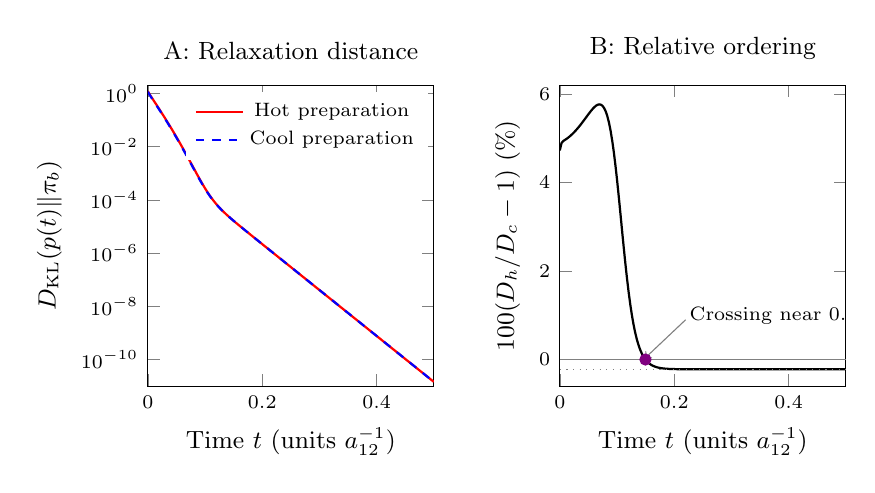
\begin{tikzpicture}
\begin{groupplot}[group style={group size=2 by 1,horizontal sep=1.6cm},width=0.43\textwidth,height=5.4cm,tick label style={font=\scriptsize},label style={font=\small},title style={font=\small},xlabel={Time $t$ (units $a_{12}^{-1}$)},xmin=0,xmax=.5]
\nextgroupplot[title={A: Relaxation distance},ymode=log,ymin=1e-11,ymax=2,ytick={1,1e-2,1e-4,1e-6,1e-8,1e-10},ylabel={$D_{\rm KL}(p(t)\Vert\pi_b)$},legend style={font=\scriptsize,draw=none,at={(.98,.98)},anchor=north east}]
\addplot[red,thick] coordinates {(0,1.21013788612) (0.004297994269,0.842995461777) (0.008595988539,0.608987398936) (0.01289398281,0.440341581659) (0.01719197708,0.317610499322) (0.02148997135,0.228359408254) (0.02578796562,0.163590181022) (0.03008595989,0.116712896394) (0.03438395415,0.0828931212786) (0.03868194842,0.0585837956434) (0.04297994269,0.0411839769259) (0.04727793696,0.0287887239354) (0.05157593123,0.0200052178145) (0.0558739255,0.0138173290506) (0.06017191977,0.0094857680391) (0.06446991404,0.00647444487958) (0.06876790831,0.00439616683326) (0.07306590258,0.00297261554659) (0.07736389685,0.00200487053096) (0.08166189112,0.00135171854244) (0.08595988539,0.000913707520456) (0.09025787966,0.000621437483811) (0.09455587393,0.000426978003437) (0.09885386819,0.000297596870429) (0.1031518625,0.000211201716764) (0.1074498567,0.000153053858448) (0.111747851,0.000113426372608) (0.1160458453,8.59590776246e-05) (0.1203438395,6.65220464343e-05) (0.1246418338,5.24440941518e-05) (0.1289398281,4.19979987345e-05) (0.1332378223,3.40624669361e-05) (0.1375358166,2.79032297638e-05) (0.1418338109,2.30328834405e-05) (0.1461318052,1.91219036217e-05) (0.1504297994,1.59424477581e-05) (0.1547277937,1.33329329201e-05) (0.159025788,1.11756708466e-05) (0.1633237822,9.38266728223e-06) (0.1676217765,7.88651546087e-06) (0.1719197708,6.63447149767e-06) (0.176217765,5.58452620241e-06) (0.1805157593,4.70273986701e-06) (0.1848137536,3.96138595297e-06) (0.1891117479,3.33762156401e-06) (0.1934097421,2.81250823938e-06) (0.1977077364,2.37027154024e-06) (0.2020057307,1.99772792466e-06) (0.2063037249,1.68383221109e-06) (0.2106017192,1.41931443341e-06) (0.2148997135,1.19638469923e-06) (0.2191977077,1.00849096794e-06) (0.223495702,8.50118800469e-07) (0.2277936963,7.1662491024e-07) (0.2320916905,6.040982621e-07) (0.2363896848,5.09243827335e-07) (0.2406876791,4.292850983e-07) (0.2449856734,3.61882214057e-07) (0.2492836676,3.05063124171e-07) (0.2535816619,2.57165670569e-07) (0.2578796562,2.16788829415e-07) (0.2621776504,1.82751648505e-07) (0.2664756447,1.5405865608e-07) (0.270773639,1.29870715468e-07) (0.2750716332,1.09480464761e-07) (0.2793696275,9.22916181458e-08) (0.2836676218,7.78015204764e-08) (0.287965616,6.55864430043e-08) (0.2922636103,5.52891890983e-08) (0.2965616046,4.66086467801e-08) (0.3008595989,3.92909821095e-08) (0.3051575931,3.31222156051e-08) (0.3094555874,2.79219644352e-08) (0.3137535817,2.35381672681e-08) (0.3180515759,1.984263745e-08) (0.3223495702,1.67273144245e-08) (0.3266475645,1.41011037445e-08) (0.3309455587,1.18872132503e-08) (0.335243553,1.00209075023e-08) (0.3395415473,8.44761479409e-09) (0.3438395415,7.12133138393e-09) (0.3481375358,6.00327627651e-09) (0.3524355301,5.06075721525e-09) (0.3567335244,4.26621472219e-09) (0.3610315186,3.59641623017e-09) (0.3653295129,3.03177674123e-09) (0.3696275072,2.5557861454e-09) (0.3739255014,2.1545264534e-09) (0.3782234957,1.81626482611e-09) (0.38252149,1.53111050007e-09) (0.3868194842,1.29072557705e-09) (0.3911174785,1.08808122076e-09) (0.3954154728,9.17252131338e-10) (0.399713467,7.73243288105e-10) (0.4040114613,6.51843894075e-10) (0.4083094556,5.49504251606e-10) (0.4126074499,4.63231968835e-10) (0.4169054441,3.90504461927e-10) (0.4212034384,3.29195194641e-10) (0.4255014327,2.77511498414e-10) (0.4297994269,2.33942154795e-10) (0.4340974212,1.9721320751e-10) (0.4383954155,1.66250712102e-10) (0.4426934097,1.40149333914e-10) (0.446991404,1.18145876234e-10) (0.4512893983,9.95969645406e-11) (0.4555873926,8.39602343497e-11) (0.4598853868,7.07784725827e-11) (0.4641833811,5.96662487535e-11) (0.4684813754,5.02986450691e-11) (0.4727793696,4.24017559113e-11) (0.4770773639,3.57446789062e-11) (0.4813753582,3.01327634e-11) (0.4856733524,2.54019189279e-11) (0.4899713467,2.14138172552e-11) (0.494269341,1.80518477013e-11) (0.4985673352,1.52177074778e-11) (0.5,1.43755705045e-11)};\addlegendentry{Hot preparation}
\addplot[blue,dashed,thick] coordinates {(0,1.1554895572) (0.004297994269,0.803461576189) (0.008595988539,0.580185474244) (0.01289398281,0.419364575234) (0.01719197708,0.302354194621) (0.02148997135,0.217286688894) (0.02578796562,0.155575093154) (0.03008595989,0.110929645075) (0.03438395415,0.0787358757628) (0.03868194842,0.0556082906007) (0.04297994269,0.0390647635126) (0.04727793696,0.0272877691897) (0.05157593123,0.0189487897175) (0.0558739255,0.0130789599167) (0.06017191977,0.00897369130476) (0.06446991404,0.00612233088008) (0.06876790831,0.00415629420604) (0.07306590258,0.00281084148171) (0.07736389685,0.00189692923778) (0.08166189112,0.00128049982498) (0.08595988539,0.000867258167281) (0.09025787966,0.000591495738387) (0.09455587393,0.000407901651071) (0.09885386819,0.000285582655926) (0.1031518625,0.000203720946556) (0.1074498567,0.000148448546014) (0.111747851,0.000110624197399) (0.1160458453,8.42754713897e-05) (0.1203438395,6.55252253156e-05) (0.1246418338,5.18646974948e-05) (0.1289398281,4.16696612046e-05) (0.1332378223,3.38833734381e-05) (0.1375358166,2.78116075661e-05) (0.1418338109,2.29915772606e-05) (0.1461318052,1.91087726656e-05) (0.1504297994,1.59444421841e-05) (0.1547277937,1.3342468424e-05) (0.159025788,1.11884247183e-05) (0.1633237822,9.39624667441e-06) (0.1676217765,7.89965729757e-06) (0.1719197708,6.64656461516e-06) (0.176217765,5.59532783414e-06) (0.1805157593,4.71220880055e-06) (0.1848137536,3.96958540287e-06) (0.1891117479,3.34466348692e-06) (0.1934097421,2.81852213046e-06) (0.1977077364,2.37538757317e-06) (0.2020057307,2.00206840073e-06) (0.2063037249,1.68750774255e-06) (0.2106017192,1.42242275658e-06) (0.2148997135,1.19901088906e-06) (0.2191977077,1.01070834563e-06) (0.223495702,8.51990133239e-07) (0.2277936963,7.18203682565e-07) (0.2320916905,6.05429902655e-07) (0.2363896848,5.10366836116e-07) (0.2406876791,4.30232052248e-07) (0.2449856734,3.62680647913e-07) (0.2492836676,3.05736292829e-07) (0.2535816619,2.57733203551e-07) (0.2578796562,2.17267289645e-07) (0.2621776504,1.83155007565e-07) (0.2664756447,1.54398697361e-07) (0.270773639,1.30157375524e-07) (0.2750716332,1.0972212196e-07) (0.2793696275,9.24953365351e-08) (0.2836676218,7.79732556769e-08) (0.287965616,6.57312159652e-08) (0.2922636103,5.54112326839e-08) (0.2965616046,4.67115294085e-08) (0.3008595989,3.9377712018e-08) (0.3051575931,3.31953287689e-08) (0.3094555874,2.7983598696e-08) (0.3137535817,2.35901248321e-08) (0.3180515759,1.98864375779e-08) (0.3223495702,1.67642378516e-08) (0.3266475645,1.41322301285e-08) (0.3309455587,1.19134527402e-08) (0.335243553,1.00430273512e-08) (0.3395415473,8.46626179447e-09) (0.3438395415,7.13705077999e-09) (0.3481375358,6.01652770769e-09) (0.3524355301,5.0719281564e-09) (0.3567335244,4.27563181367e-09) (0.3610315186,3.60435482906e-09) (0.3653295129,3.03846897295e-09) (0.3696275072,2.56142769121e-09) (0.3739255014,2.15928227225e-09) (0.3782234957,1.82027397811e-09) (0.38252149,1.53449021265e-09) (0.3868194842,1.2935746728e-09) (0.3911174785,1.09048300697e-09) (0.3954154728,9.19276835952e-10) (0.399713467,7.74950113201e-10) (0.4040114613,6.53282746945e-10) (0.4083094556,5.50717204048e-10) (0.4126074499,4.64254487339e-10) (0.4169054441,3.91366444716e-10) (0.4212034384,3.29921845895e-10) (0.4255014327,2.7812406524e-10) (0.4297994269,2.34458548491e-10) (0.4340974212,1.9764852729e-10) (0.4383954155,1.66617686596e-10) (0.4426934097,1.40458693352e-10) (0.446991404,1.18406666193e-10) (0.4512893983,9.98168104413e-11) (0.4555873926,8.41455644174e-11) (0.4598853868,7.09347058098e-11) (0.4641833811,5.97979533491e-11) (0.4684813754,5.0409672032e-11) (0.4727793696,4.24953516327e-11) (0.4770773639,3.58235800932e-11) (0.4813753582,3.01992770962e-11) (0.4856733524,2.54579899704e-11) (0.4899713467,2.14610851417e-11) (0.494269341,1.80916945279e-11) (0.4985673352,1.52512983514e-11) (0.5,1.44073024831e-11)};\addlegendentry{Cool preparation}
\nextgroupplot[title={B: Relative ordering},ylabel={$100(D_h/D_c-1)$ (\%)},ymin=-.6,ymax=6.2]
\addplot[black,thick] coordinates {(0,4.72945242796) (0.002865329513,4.89158842429) (0.005730659026,4.93838902716) (0.008595988539,4.96426159744) (0.01146131805,4.98892905107) (0.01432664756,5.01595684521) (0.01719197708,5.04583861343) (0.02005730659,5.07853498975) (0.0229226361,5.11393161062) (0.02578796562,5.15190941246) (0.02865329513,5.19234463846) (0.03151862464,5.23509603344) (0.03438395415,5.27998891932) (0.03724928367,5.32679719851) (0.04011461318,5.37522281625) (0.04297994269,5.42487198877) (0.04584527221,5.4752275317) (0.04871060172,5.52561674363) (0.05157593123,5.57517452435) (0.05444126074,5.62280178951) (0.05730659026,5.66711985913) (0.06017191977,5.70642244031) (0.06303724928,5.73862820073) (0.0659025788,5.76123884197) (0.06876790831,5.77131009811) (0.07163323782,5.76544617307) (0.07449856734,5.73983155693) (0.07736389685,5.69031733132) (0.08022922636,5.61258084449) (0.08309455587,5.50237615175) (0.08595988539,5.35588535542) (0.0888252149,5.17016528956) (0.09169054441,4.94365846468) (0.09455587393,4.67670388594) (0.09742120344,4.3719502183) (0.100286533,4.03455512448) (0.1031518625,3.67206727382) (0.106017192,3.29394163068) (0.1088825215,2.91072690005) (0.111747851,2.53305811393) (0.1146131805,2.1706483271) (0.11747851,1.8314729471) (0.1203438395,1.52127842967) (0.1232091691,1.24345246791) (0.1260744986,0.999204660263) (0.1289398281,0.787953442396) (0.1318051576,0.607803886449) (0.1346704871,0.456021168678) (0.1375358166,0.329438697433) (0.1404011461,0.224773429427) (0.1432664756,0.138845874155) (0.1461318052,0.0687168997329) (0.1489971347,0.011759483314) (0.1518624642,-0.0343160525548) (0.1547277937,-0.0714673148158) (0.1575931232,-0.101343199991) (0.1604584527,-0.125316431572) (0.1633237822,-0.144519324029) (0.1661891117,-0.159879081081) (0.1690544413,-0.172150543859) (0.1719197708,-0.18194538362) (0.1747851003,-0.18975741719) (0.1776504298,-0.195984128036) (0.1805157593,-0.200944693858) (0.1833810888,-0.20489492013) (0.1862464183,-0.208039504929) (0.1891117479,-0.210542045055) (0.1919770774,-0.212533156905) (0.1948424069,-0.214117040194) (0.1977077364,-0.215376765843) (0.2005730659,-0.216378524956) (0.2034383954,-0.217175035928) (0.2063037249,-0.217808271964) (0.2091690544,-0.218311641636) (0.212034384,-0.218711730305) (0.2148997135,-0.219029689635) (0.217765043,-0.219282345544) (0.2206303725,-0.219483081147) (0.223495702,-0.219642540063) (0.2263610315,-0.219769186431) (0.229226361,-0.219869750693) (0.2320916905,-0.219949584356) (0.2349570201,-0.220012942266) (0.2378223496,-0.22006320717) (0.2406876791,-0.220103068339) (0.2435530086,-0.220134663631) (0.2464183381,-0.22015969248) (0.2492836676,-0.22017950574) (0.2521489971,-0.220195177131) (0.2550143266,-0.220207560044) (0.2578796562,-0.220217332713) (0.2607449857,-0.220225034124) (0.2636103152,-0.220231092572) (0.2664756447,-0.220235848355) (0.2693409742,-0.220239571828) (0.2722063037,-0.220242477746) (0.2750716332,-0.220244736672) (0.2779369628,-0.220246484044) (0.2808022923,-0.220247827385) (0.2836676218,-0.220248852033) (0.2865329513,-0.220249625696) (0.2893982808,-0.220250202072) (0.2922636103,-0.22025062373) (0.2951289398,-0.220250924397) (0.2979942693,-0.220251130777) (0.3008595989,-0.220251263996) (0.3037249284,-0.22025134075) (0.3065902579,-0.220251374221) (0.3094555874,-0.220251374801) (0.3123209169,-0.220251350667) (0.3151862464,-0.220251308242) (0.3180515759,-0.220251252559) (0.3209169054,-0.220251187546) (0.323782235,-0.220251116263) (0.3266475645,-0.220251041076) (0.329512894,-0.220250963809) (0.3323782235,-0.220250885855) (0.335243553,-0.220250808268) (0.3381088825,-0.220250731836) (0.340974212,-0.220250657136) (0.3438395415,-0.220250584586) (0.3467048711,-0.220250514471) (0.3495702006,-0.220250446981) (0.3524355301,-0.220250382226) (0.3553008596,-0.220250320261) (0.3581661891,-0.220250261093) (0.3610315186,-0.220250204697) (0.3638968481,-0.220250151022) (0.3667621777,-0.2202501) (0.3696275072,-0.220250051549) (0.3724928367,-0.220250005577) (0.3753581662,-0.22024996199) (0.3782234957,-0.220249920688) (0.3810888252,-0.22024988157) (0.3839541547,-0.220249844537) (0.3868194842,-0.220249809489) (0.3896848138,-0.220249776329) (0.3925501433,-0.220249744964) (0.3954154728,-0.220249715303) (0.3982808023,-0.220249687258) (0.4011461318,-0.220249660744) (0.4040114613,-0.220249635681) (0.4068767908,-0.220249611993) (0.4097421203,-0.220249589605) (0.4126074499,-0.220249568448) (0.4154727794,-0.220249548456) (0.4183381089,-0.220249529564) (0.4212034384,-0.220249511714) (0.4240687679,-0.220249494849) (0.4269340974,-0.220249478915) (0.4297994269,-0.22024946386) (0.4326647564,-0.220249449636) (0.435530086,-0.220249436199) (0.4383954155,-0.220249423504) (0.441260745,-0.220249411511) (0.4441260745,-0.220249400181) (0.446991404,-0.220249389478) (0.4498567335,-0.220249379366) (0.452722063,-0.220249369814) (0.4555873926,-0.22024936079) (0.4584527221,-0.220249352265) (0.4613180516,-0.220249344212) (0.4641833811,-0.220249336604) (0.4670487106,-0.220249329418) (0.4699140401,-0.220249322629) (0.4727793696,-0.220249316215) (0.4756446991,-0.220249310157) (0.4785100287,-0.220249304434) (0.4813753582,-0.220249299027) (0.4842406877,-0.22024929392) (0.4871060172,-0.220249289095) (0.4899713467,-0.220249284537) (0.4928366762,-0.220249280232) (0.4957020057,-0.220249276164) (0.4985673352,-0.220249272322) (0.5,-0.220249270481)};
\addplot[gray] coordinates {(0,0)(.5,0)};
\addplot[gray,dotted] coordinates {(0,-.2202492067)(.5,-.2202492067)};
\addplot[only marks,violet,mark=*] coordinates {(.1496723312,0)};
\node[font=\scriptsize,anchor=west] at (axis cs:.21,1) {Crossing near $0.14967$};
\draw[->,gray] (axis cs:.22,.9) -- (axis cs:.1496723312,.04);
\end{groupplot}
\end{tikzpicture}
\caption{Actual evolution $p(t)=e^{tM}\pi(\beta)$ for the same two preparations. Relative entropy decreases for each, and the hotter state's distance becomes smaller. The ratio panel resolves the crossing that is difficult to see on the logarithmic plot. The horizontal dotted line is the asymptotic ratio difference, $-0.2202492\%$. Rational uniformization and logarithm bounds certify opposite KL orderings at $t=0.14$ and $0.16$; the displayed root location is numerical, with no claim of uniqueness.}
\label{fig:crossing}
\end{figure}


The relevant fractional amplitude reduction is
\[
\epsilon_b=1-\frac{|b_h|}{|b_c|}\simeq0.0011018531=0.11018531\%.
\]
For relative entropy the leading term is quadratic, so
\[
1-\lim_{t\to\infty}\frac{D_h(t)}{D_c(t)}
=1-\frac{b_h^2}{b_c^2}\simeq0.22024921\%.
\]
Both preparations have the same decay exponent $\lambda_2$. This is an ordinary effect, not the exponentially faster strong effect. For an increasingly small common distance threshold, the asymptotic time advance is
\[
\Delta t=\frac{\log(|b_c|/|b_h|)}{|\lambda_2|}
\simeq5.5488\,10^{-5}\,a_{12}^{-1}.
\]
The slow relaxation time is $1/|\lambda_2|\simeq0.0503313\,a_{12}^{-1}$, so this advance is only about $0.11025\%$ of one slow relaxation time. It is not a percentage reduction in the full cooling time, which depends on the chosen threshold. The time unit has no assigned experimental value, and $T_h/T_b=1000$, $T_c/T_b=100$. These data establish a strict mathematical failure of the triplet inference; they do not establish a practically useful cooling protocol.

\subsection{Triplet-rate applications of stochastic monotonicity}
Let $L=M^\top$ act on functions, $(Lf)_i=\sum_{j\ne i}a_{ji}(f_j-f_i)$. Define adjacent differences $y_i=f_{i+1}-f_i$, the difference map $Bf=y$, and $(H_0y)_j=\sum_{\ell<j}y_\ell$. Then $BL=KB$ with $K=BLH_0$, since $L\mathbf1=0$. In the constant-plus-differences basis, $L$ is block triangular with blocks 0 and $K$, so $K$ has precisely the nonzero generator eigenvalues. For its off-diagonal entries,
\[
K_{i\ell}=\begin{cases}
\sum_{j\leq\ell}(a_{j,i}-a_{j,i+1}),&\ell<i,\\
\sum_{j>\ell}(a_{j,i+1}-a_{j,i}),&\ell>i.
\end{cases}
\]
\begin{theorem}[Application of stochastic monotonicity]
For any finite number of states, strictly ordered energies, a fixed $0<\beta_b<\infty$, positive reversible rates and a simple slowest nonzero eigenvalue, if every off-diagonal entry of $K$ is nonnegative, there is no asymptotic cooling or heating Mpemba effect at positive initial temperatures.
\end{theorem}
\begin{proof}
Such a matrix $K$ is called Metzler. After a sufficiently large scalar diagonal shift it is nonnegative. Perron theory gives a nonzero nonnegative eigenvector $y$ at its spectral abscissa, which is $\lambda_2$. This does not require irreducibility of $K$. Choose $w$ with $Bw=y$ and $\pi_b^\top w=0$. Then $B(Lw-\lambda_2w)=0$, so $Lw-\lambda_2w$ is constant. Its bath expectation is zero, hence it vanishes. Thus $w$ is the slow left eigenfunction, nondecreasing and nonconstant in energy.

The covariance identity now gives $b_2'(\beta)<0$ for every finite positive $\beta$: all its pairwise summands are nonnegative and at least one is strictly positive. Because $b_2(\beta_b)=0$, its absolute value decreases toward the bath on the cooling side and increases away from the bath on the heating side. These are exactly the normal asymptotic orderings.
\end{proof}
In four states, the six off-diagonal entries are
\begin{align*}
K_{12}&=a_{32}+a_{42}-a_{31}-a_{41},&K_{13}&=a_{42}-a_{41},\\
K_{21}&=a_{12}-a_{13},&K_{23}&=a_{43}-a_{42},\\
K_{31}&=a_{13}-a_{14},&K_{32}&=a_{13}+a_{23}-a_{14}-a_{24}.
\end{align*}
The original failures already ensure the three upper entries are nonnegative, since $G\leq0$ orders upward rates. A corrected, directly checkable sufficient condition is therefore the four original failures together with
\[
a_{12}\geq a_{13},\qquad a_{13}\geq a_{14},\qquad
 a_{13}+a_{23}\geq a_{14}+a_{24}.
\]
This is a proved sufficient condition, not a proposed necessary characterization.

\begin{corollary}
If every triplet has $\kappa\leq1$ and fails the original predicate, then the absence conclusion is true, for any state count under the theorem's assumptions.
\end{corollary}
\begin{proof}
$H\leq0$ and $G\leq0$ give $A+B\leq C(1+t)$ and $B\geq At$, so $A\leq C$. These comparisons make each downward summand in $K$ nonnegative; $G\leq0$ and detailed balance do the same for each upward summand. Apply the theorem.
\end{proof}
A second subfamily consists of downward gap laws $a_{ij}=f(E_j-E_i)$, $i<j$, with positive nonincreasing $f$. Both $f(x)$ and $e^{-\beta_bx}f(x)$ are nonincreasing, so every required summand is nonnegative. This establishes the same absence conclusion directly, without the false general triplet conjecture. The following comparison locates this argument within established order theory; no general monotonicity novelty is claimed.

\subsection{Relation to earlier no-Mpemba theorems}\label{sec:priororder}
\href{https://arxiv.org/html/2410.06623v2}{Ohga, Hayakawa and Ito (OHI), Result 2 and SI D} already use monotone coupling to exclude Mpemba behavior. Their SI D2 explicitly treats a total order. Our matrix condition is precisely a finite-chain expression of stochastic monotonicity, not a separate physical principle. The relevant distinctions are:
\begin{center}\small
\begin{tabular}{p{.17\textwidth}p{.36\textwidth}p{.36\textwidth}}
\toprule &OHI Result 2&The preceding spectral criterion\\\midrule
State order&Finite partial order; energy respects it&Total order by distinct energies\\
Dynamics&Irreducible and Gibbs-stationary; reversibility unnecessary&Positive reversible rates\\
Order condition&Comparable jumps and a monotone coupling&$K=BLH_0$ is Metzler\\
Bath range&Hypotheses throughout a temperature interval&One fixed finite positive bath\\
Spectrum&No simplicity requirement&Simple slowest nonzero eigenvalue\\
Conclusion&No cooling mean-energy crossing at any time&No asymptotic cooling/heating reversal in fixed norms or KL\\\bottomrule
\end{tabular}
\end{center}
OHI SI B extends their Result 1, the microscopic characterization, to KL divergence; it does not state Result 2 as an all-time KL theorem. Thus the different observable and time scopes must not be conflated.

Indeed $BL=KB$ gives $Be^{tL}=e^{tK}B$. The Metzler condition is equivalent to $e^{tL}$ preserving increasing functions: sufficiency follows from $e^{tK}\geq0$, and necessity by differentiation at zero on coordinate vectors of adjacent differences. This also gives a monotone coupling. Choose $r$ large enough that $I+L/r$ is stochastic and $I+K/r$ is entrywise nonnegative. Its transition rows are stochastically ordered. A common Poisson clock of rate $r$ and common-uniform inverse-CDF updates preserve the order of two copies. On a total order, energy compatibility and comparability of jumps are automatic.

For fixed bath, $e^{tL}E$ is then increasing, so
\[
\partial_\beta\{\pi(\beta)^\top e^{tL}E\}
=-\Cov_{\pi(\beta)}(e^{tL}E,E)\leq0.
\]
This gives all-time energy ordering without reversibility or spectral simplicity. It explains the direct relation to OHI while avoiding an inference from a single observable to all possible distances.

The likelihood-ratio and stochastic-order methods below also have precedent in \href{https://arxiv.org/abs/1109.6075}{Fill and Kahn, Ann. Appl. Probab. 23 (2013), 1778--1816}, specifically Proposition 3.2, Corollary 3.3 and the density-ratio identity (3.2). They compare different kernels from a common initial law and obtain TV, separation and, with additional assumptions, weighted $L^2$ comparisons. Here one kernel acts on different Gibbs preparations. Their argument is a methodological precedent, not a verbatim statement of the corollary below. We provide the following consequence for clarity, without a priority claim.

\begin{corollary}[Application: all-time convex-divergence ordering]
Let a finite irreducible generator be reversible with positive Gibbs equilibrium, on a total energy order, and let $K$ be Metzler. For any convex $\Phi$ finite on positive arguments, with $\Phi(1)=0$, define
\[
D_\Phi(p\Vert\pi_b)=\sum_i\pi_{bi}\Phi(p_i/\pi_{bi}).
\]
For same-side Gibbs preparations, the farther initial temperature has at least as large a divergence at every $t\geq0$. This includes KL and total variation, and requires no simple eigenvalue. For KL the inequality is strict at every finite time for distinct initial temperatures.
\end{corollary}
\begin{proof}
Write $p\succeq_{\rm st}q$ when $\sum_i p_i f_i\geq\sum_i q_i f_i$ for every increasing $f$. Gibbs laws are stochastically ordered by temperature, by the pairwise covariance identity. A monotone semigroup preserves this order. Thus for cooling $p_h(t)\succeq_{\rm st}p_c(t)\succeq_{\rm st}\pi_b$.

Reversibility implies $p_c(t)/\pi_b=e^{tL}[\pi(\beta_c)/\pi_b]$ componentwise. The initial ratio is proportional to $e^{(\beta_b-\beta_c)E_i}$ and is increasing; it stays increasing. Choose a nondecreasing subgradient $g$ of $\Phi$. Convexity and stochastic order give
\[
D_\Phi(p_h\Vert\pi_b)-D_\Phi(p_c\Vert\pi_b)
\geq\sum_i(p_{hi}-p_{ci})g(p_{ci}/\pi_{bi})\geq0.
\]
For heating, $p_c\preceq_{\rm st}p_h\preceq_{\rm st}\pi_b$ and $p_h/\pi_b$ is decreasing. Apply the same supporting-line inequality at $p_h/\pi_b$ to obtain $D_\Phi(p_c\Vert\pi_b)\geq D_\Phi(p_h\Vert\pi_b)$. KL is strictly convex, and invertibility of $e^{tM}$ keeps two distinct initial distributions distinct at finite $t$, proving strictness.
\end{proof}
This does not assert all-time ordering for every arbitrary norm. The original spectral proof supplies the every-fixed-norm conclusion asymptotically with a simple slow mode. Our counterexample violates monotonicity explicitly: $K_{21}=a_{12}-a_{13}=-27$. It therefore challenges neither OHI's theorem nor this corollary.

\subsection{Broader literature assessment and contribution scope}\label{sec:novelty}
The starting contribution is the explicit, certified failure of the published original-rate triplet implication. Sections~\ref{sec:orderedconductances}--\ref{sec:degenerateextension} add a surviving all-dimension exclusion theorem and a finite four-state asymptotic classification; their precise novelty is assessed separately from the established tools used in their proofs. Section~\ref{sec:mechanism} also supplies a controlled family and a proved onset classification for a specified eigenvector geometry. This is a problem-specific structural result; its individual publication priority has not been established. The supporting results organize and apply established mathematics. The following comparison was checked on 11 October 2026; it separates mathematical validity from publication priority.

\paragraph{The matrix criterion and reset algebra have direct precedents.}
\href{https://arxiv.org/abs/2007.11433v3}{Baake and Sumner, \emph{On equal-input and monotone Markov matrices}, v3, 25 September 2022}, Fact 3.1 and Proposition 3.11, give the cumulative-coordinate characterization of stochastic monotonicity for matrices and generators. In their row-generator convention, let $T_{ij}=\mathbf1_{i\geq j}$. Its coordinates are $(f_1,Bf)$, so
\[
T^{-1}LT=\begin{pmatrix}0&*\\0&K\end{pmatrix}.
\]
The upper row outside the diagonal consists of outgoing-rate tail sums and is automatically nonnegative. Their transformed-generator criterion is therefore exactly our condition that $K$ is Metzler. Our Perron and covariance argument is an application of that order structure, not a new monotonicity criterion.

Their Section 2.1 also treats equal-input generators $C-cI$, with identical rows in $C$ and $C^2=cC$. Our reset generator is the transpose of this construction, with $C=\mathbf1\pi_b^\top$ and $c=1$. Its scalar action on nonstationary modes is elementary equal-input algebra. The useful calculation here is its compatibility with the particular triplet inequalities, $F(R_0)=G(R_0)=0$; the general reset construction is not claimed as new.

\paragraph{The divergence corollary also follows from established thermomajorization.}
\href{https://arxiv.org/html/2410.06686v2}{Vu and Hayakawa, \emph{Thermomajorization Mpemba Effect}, v2, 6 January 2025}, give the Lorenz-curve and all-convex-divergence characterizations of thermomajorization. The connection to our corollary is explicit. In cooling, both $p_h/\pi_b$ and $p_c/\pi_b$ are increasing, so both curves use the order $n,n-1,\ldots,1$. At their common horizontal knots,
\[
x_k=\sum_{i=k}^n\pi_{bi},\qquad
y_{h,k}=\sum_{i=k}^np_{hi}\geq\sum_{i=k}^np_{ci}=y_{c,k},
\]
by stochastic ordering. Linear interpolation orders the entire curves: $p_h$ thermomajorizes $p_c$. Heating uses the order $1,\ldots,n$ and lower-tail inequalities, so $p_c$ thermomajorizes $p_h$. This yields the corollary from the known convex-divergence characterization. The supporting-line proof above is an alternative elementary derivation; neither derivation establishes priority for a new general theorem.

This absence argument does not assert a thermomajorization reversal for our counterexample. Vu and Hayakawa's Result 4 distinguishes that stronger notion from the scalar slow-overlap criterion. The counterexample's stated conclusions remain eventual fixed-norm and KL ordering, with separate finite-time KL and TV brackets.

\paragraph{What is claimed, and what is retained only as support.}
\begin{itemize}
\item \textbf{Central result:} the four-state witness satisfying all original-rate triplet failures, its exact certification and the consequent refutation of $(\mathcal C_4)$. The checked sources do not supply this witness or settle that precise implication. This bounded finding is not an exhaustive priority guarantee.
\item \textbf{Established tools:} reversible symmetrization, slow-mode overlaps, Perron theory, stochastic monotonicity, likelihood-ratio evolution, thermomajorization, and equal-input reset algebra. The report claims no methodological novelty for these tools or for rational certification itself.
\item \textbf{Applications proved here:} the additional rate inequalities, the all-$\kappa\leq1$ subfamily, the nonincreasing gap-law subfamily, and the all-time convex-divergence corollary. Their role is to explain sufficient conditions that survive the failed conjecture. They are not promoted as independently novel theorems.
\item \textbf{Problem-specific deductions:} the identity $F=hG+dH$, the feasible-cone formulation, and reset compatibility simplify construction and verification. They are proved directly; their individual publication priority remains unestablished. The open-neighborhood result is a continuity consequence, not a new perturbation principle.
\end{itemize}

The review covers the exact source conjecture, OHI's coupling result and SI, Fill--Kahn's comparison and density-ratio argument, Baake--Sumner's matrix and generator criteria, and Vu--Hayakawa's thermomajorization formulation. Searches combined Mpemba, triplet, monotonicity, convex divergence, likelihood ratio, nonincreasing rates and equal-input generators. Relevant full-text sections were inspected, rather than inferred from titles. No identical all-lower-branch or gap-law statement was located in this bounded review; that absence is insufficient evidence of novelty. Unindexed work and exhaustive citation tracing remain outside the check. The counterexample remains a contribution independently of supporting priority questions. The added contrast-cone and classification results must be evaluated on their exact hypotheses and conclusions; the bounded search is not a guarantee that these consequences are unprecedented.

\paragraph{Additional sources for the classification and realization arguments.}
The explicit slow-mode realization is already proved in \href{https://arxiv.org/abs/1711.05829v3}{Klich et al., v3, 18 December 2018}, Appendix VIII, particularly Eq.~(67). Our rank-one formula is that construction in different normalization, and the rank-$r$ version uses the same projector idea. The Mpemba index and parity criteria are likewise prior results from that work. \href{https://arxiv.org/abs/2502.01758v3}{Teza et al., v3, 16 April 2025}, Sections 2.1 and 5.2.3, review those results. Both primary full texts were inspected on 11 October 2026. The university-hosted journal PDF failed to download; the arXiv review version was inspected instead, and differences in the final journal text have not been excluded.

The nonvanishing-Wronskian characterization of extended complete Chebyshev systems is classical; Gasull, Geyer and Ma\~nosas (2020), Lemma 2.3, states the criterion used here. The Gibbs Wronskian formula and the convex-curve test are explicit applications. The weighted Helmert basis, Metzler semigroup positivity and Perron theory are also established. What is supplied here is the rate-to-contrast identity, the resulting asymmetric cooling/heating implications of the triplet premise, and the explicit finite thermal test. Searches combining Mpemba with Helmert, conductance ordering, strong-effect absence, Chebyshev systems and stationary-point counts did not locate matching statements in the inspected primary sources. This is a bounded attribution assessment, not an exhaustive priority claim.

\paragraph{An explicit prior strong-temperature count.}
A further search located \href{https://doi.org/10.5281/zenodo.21298061}{Parker
Emmerson, \emph{Organizational Mechanics of Effective Cardinality Transitions}},
Zenodo v1, with a stated publication date of 10 July 2026 and repository creation
date of 17 July 2026. The full text was inspected on 11 October 2026.
Theorem 7.3 applies the classical sign-variation bound to the slow-overlap
numerator; Corollary 7.5 subtracts the forced bath zero. Thus the scalar
nonbath strong-temperature bound $n-2$ is explicitly present in prior work
and is not a novelty claim here. Section 11 gives a four-state sharpness example
using a preparation landscape different from the stationary one. Warning 7.13
distinguishes simultaneous mode cancellation from the scalar result.
Our rank-$r$ bound $n-r-1$ addresses that simultaneous-cancellation problem;
its priority remains subject to further review. The bound on \emph{stationary
points} and the derivative-curve classifier concern different objects from
zeros of the overlap numerator. No statement about the manuscript's peer-review
status is needed for this attribution.

The coexistence of strong cooling and heating in four states is also prior
work: \href{https://arxiv.org/abs/2308.04557v1}{Bera, Walker and Vucelja,
v1, 8 August 2023}, Section IV and Fig.~4, give a four-state ring example and
discuss nonoverlap of the strong effects in three states. Those passages
were checked in the primary full text on 11 October 2026. Our rational
coexistence example is a sharpness and verification construction, not the
first observation of that phenomenon. The general derivative test also
covers ordinary effects that need not cancel the slow mode.

\paragraph{The sharp full-triplet conclusions.}
The additional results in Sections~\ref{sec:fulltripletbound} and
\ref{sec:tripletendpoint} concern the precise original-rate premise:
a sharp $25\%$ amplitude-advantage supremum and an exact endpoint covariance
criterion for ordinary cooling. Their proofs use a restriction on the first
three components of the slow eigenfunction, established through a reversible
Schur complement and three nonnegative-rate boundary faces. A separate
Perron-coupling proof supports the same restriction. These are proposed
problem-specific contributions, not new Schur-complement or Perron principles.
Searches combining Mpemba with amplitude bounds, triplet constraints,
four-state systems and energy-span thresholds located no matching theorem
in the inspected primary sources. Expert assessment of priority remains
necessary. The spacing-independent exclusion also explains why the March
paper's finite-temperature sampling box lies entirely within a region where
the original inference is valid.

\section{What the triplet premise still guarantees in any dimension}\label{sec:orderedconductances}
The counterexample invalidates the proposed exclusion of ordinary cooling.
A substantial part of the exclusion principle nevertheless survives, under
only the $G$ inequalities and for any number of states.

Let $q_i=\pi_i(\beta_b)>0$ and define the symmetric reduced conductances
\[
k_{ij}=\frac{M_{ij}}{q_i}=\frac{M_{ji}}{q_j},\qquad i\ne j.
\]
These are conductances divided by both equilibrium weights. For an ordered
triplet $i<j<k$, its original-rate expression is
$G_{ijk}=a_{ik}q_j/q_i-a_{jk}=q_j(k_{ik}-k_{jk})$. Thus the condition
\begin{equation}\label{eq:orderedk}
k_{ik}\leq k_{jk}\quad\text{for all }i<j<k
\end{equation}
is exactly $G_{ijk}\leq0$ for every triplet. Failure of every original
predicate implies this condition, by the branch-equivalence lemma. No
$F$ inequality is used in the following theorem.

\begin{theorem}[No strong effect and no anomalous heating]\label{thm:orderedk}
Consider an irreducible reversible $n$-state generator, $n\geq2$, with distinct ordered
energies and $0<\beta_b<\infty$. Suppose \eqref{eq:orderedk} holds.
Then:
\begin{enumerate}
\item No nonbath Gibbs preparation at a finite positive temperature has zero
projection onto the entire slowest nonstationary eigenspace. Hence there is
no strong cooling or strong heating effect, including when that eigenspace
is degenerate.
\item For any $\beta_f>\beta_n>\beta_b$ and every finite $t\geq0$,
\[
\sum_i\frac{[p_i(t;\beta_f)-q_i]^2}{q_i}
>
\sum_i\frac{[p_i(t;\beta_n)-q_i]^2}{q_i}.
\]
Thus heating has no finite-time weighted Euclidean reversal. It also has
no asymptotic relative-entropy reversal, for any slow multiplicity.
\item If the slow mode is simple, its thermal overlap can be oriented to be
strictly negative throughout cooling, strictly positive throughout heating,
and strictly increasing throughout heating. Consequently there is no
asymptotic heating effect in any fixed norm.
\end{enumerate}
These statements do not exclude ordinary cooling, and do not assert
finite-time relative-entropy or total-variation ordering.
\end{theorem}

\begin{proof}
Write $L=M^\top$, $Q_k=\sum_{i=1}^kq_i$, and define the weighted prefix
contrasts, for $k=1,\ldots,n-1$, by
\[
h^{(k)}_i=\begin{cases}
1,&i\leq k,\\
-Q_k/q_{k+1},&i=k+1,\\
0,&i>k+1.
\end{cases}
\]
They have zero $q$-mean and are mutually orthogonal in
$\langle f,g\rangle_q=\sum_iq_if_ig_i$. Their squared norms are
$\eta_k=Q_kQ_{k+1}/q_{k+1}$. Put $e^{(k)}=h^{(k)}/\sqrt{\eta_k}$.
This is a weighted Helmert basis of the entire nonstationary function space.

Detailed balance makes the matrix $A_{kl}=\langle e^{(k)},Le^{(l)}\rangle_q$
symmetric. For $k<l$, direct multiplication gives
\begin{align}\label{eq:helmertoffdiag}
\sqrt{\eta_k\eta_l}A_{kl}
={}&Q_{l+1}\sum_{i=1}^kq_i(k_{k+1,l+1}-k_{i,l+1})\\
&+\sum_{j=l+2}^nq_j\sum_{i=1}^kq_i(k_{k+1,j}-k_{ij})\geq0.\nonumber
\end{align}
To check the identity, note that for every $i\leq k+1\leq l$,
$(Lh^{(l)})_i=-Q_{l+1}k_{i,l+1}-\sum_{j=l+2}^nq_jk_{ij}$.
The weighted contrast subtracts its value at $i=k+1$ from the weighted
prefix values. Each resulting difference is nonnegative by
\eqref{eq:orderedk}. Thus $A$ is a symmetric Metzler matrix. In particular
$e^{tA}$ is entrywise nonnegative for $t\geq0$, with positive diagonal.
This follows by choosing $c$ so that $A+cI$ is entrywise nonnegative and
using the exponential power series.

Let $g_k(\beta)=\sum_i e^{(k)}_i\pi_i(\beta)$. Apart from its positive
normalization $\sqrt{\eta_k}$, its numerator is
\begin{align*}
N_k(\beta)
&=\sum_{i=1}^k e^{-\beta E_i}-\frac{Q_k}{q_{k+1}}e^{-\beta E_{k+1}}\\
&=e^{-\beta E_{k+1}}\sum_{i=1}^k
\left[e^{\beta(E_{k+1}-E_i)}-e^{\beta_b(E_{k+1}-E_i)}\right].
\end{align*}
Every gap in this sum is strictly positive. Therefore every coordinate
$g_k$ is strictly negative for $\beta<\beta_b$, zero at the bath, and
strictly positive for $\beta>\beta_b$.

Each $g_k$ is also strictly increasing on the heating side. Indeed, put
\[
T_k=(1+Q_k/q_{k+1})e^{-\beta E_{k+1}}+
\sum_{j=k+2}^ne^{-\beta E_j},\qquad Z=N_k+T_k.
\]
For $\beta>\beta_b$, both $N_k,T_k$ are positive and
\[
\frac{N_k'}{N_k}>-E_{k+1},\qquad
\frac{T_k'}{T_k}\leq-E_{k+1}.
\]
The first inequality follows by differentiating the positive bracketed sum
in $N_k$; the second is its interpretation as the negative weighted average
of energies at least $E_{k+1}$. Consequently
$(N_k/Z)'=(N_k'T_k-N_kT_k')/Z^2>0$.

The Gibbs likelihood ratio expands as
$\pi(\beta)/q=\mathbf1+\sum_k g_k(\beta)e^{(k)}$.
Under the reversible evolution its nonconstant coordinate vector becomes
$e^{tA}g(\beta)$. For two heating preparations farther and nearer the bath,
$g(\beta_f)>g(\beta_n)>0$ entrywise. The nonnegative matrix $e^{tA}$ with
positive diagonal preserves both strict inequalities. Taking squared
Euclidean norms of the coordinate vectors proves the finite-time assertion.

For the slow-space conclusions let $\lambda_2$ be the largest eigenvalue
of $A$ and let $\Pi_2$ be its orthogonal spectral projector. Symmetry gives
\[
\Pi_2=\lim_{t\to\infty}e^{-\lambda_2t}e^{tA}.
\]
Hence $\Pi_2$ is entrywise nonnegative and nonzero. Since $g(\beta)$ has
strictly one sign in every coordinate, $\Pi_2g(\beta)\ne0$ for every
nonbath $\beta$. This proves absence of strong effects without assuming
simplicity. Moreover $\|\Pi_2g(\beta)\|^2$ is strictly increasing on the
heating side: its derivative is
$2(\Pi_2g)^\top(\Pi_2g')>0$. Strictness follows from any positive diagonal
entry of the nonzero nonnegative projector, since $g,g'>0$. The same
quantity controls the leading relative-entropy coefficient.

If the slow mode is simple, Perron theory for a symmetric Metzler matrix
allows its coordinate eigenvector $v$ to be chosen nonnegative and nonzero.
Then $b_2(\beta)=v^\top g(\beta)$ has the stated signs and heating
monotonicity. Its scale does not affect any ordering conclusion.
\end{proof}

\paragraph{A larger rate family.}
The proof in fact requires only that the right-hand side of
\eqref{eq:helmertoffdiag} be nonnegative for each $k<l$; the individual
conductance inequalities are sufficient, but not necessary. In four states
this larger, explicitly checkable family is given by just three inequalities:
\begin{align*}
Q_3(k_{23}-k_{13})+q_4(k_{24}-k_{14})&\geq0,\\
k_{24}-k_{14}&\geq0,\\
(q_1+q_2)k_{34}-q_1k_{14}-q_2k_{24}&\geq0.
\end{align*}
Every conclusion of Theorem~\ref{thm:orderedk} holds under these three
aggregate inequalities. More generally there are $(n-1)(n-2)/2$ linear
aggregate inequalities. They can be evaluated before any eigendecomposition.

For a simple four-state slow mode in this family, the anomalous cooling
region $\{\beta\in(0,\beta_b):\partial_\beta|b_2|>0\}$ is either empty or
one connected interval. Indeed $b_2<0$ on cooling and $b_2'>0$ throughout
heating, while the global derivative bound allows at most two stationary
points counting multiplicity. The negative set of $b_2'$ before the bath can therefore have at most
one connected component. In this larger family its left endpoint is not
determined by the present argument. Under the original full triplet premise,
Corollary~\ref{cor:tripletendpoint} proves that any such interval starts at
$\beta=0$ and supplies an exact endpoint criterion.

\paragraph{A corrected implication and its mechanism.}
For every finite $n$, failure of all the original triplet predicates excludes
strong effects and excludes asymptotic heating in relative entropy; with a
simple slow mode, heating is excluded in every fixed norm. The finite-time
weighted Euclidean statement is stronger for its specified distance. The
four-state counterexample therefore occupies a precise remaining possibility:
ordinary cooling without eliminating the slow mode. Its small thermal maximum
is compatible with a slow overlap that never changes sign on either side of
the bath.

The proof uses a different order structure from monotone energy eigenvectors.
A positive combination of prefix contrasts can have nonmonotone components,
so the counterexample does not conflict with this cone. Nevertheless its
weighted prefix sums are nonnegative. More directly, every Gibbs preparation
on one side of the bath has coordinates of the same sign in this basis; a
nonnegative slow spectral projector cannot cancel all of them. This is the
mechanism excluding strong effects. On heating, all those coordinates also
grow with the distance from the bath, which explains the additional exclusion.
The basis, Metzler positivity, and Perron theory are established tools; the
specific rate-to-contrast identity and its Mpemba consequences require a
separate priority assessment.

\section{A finite-time convex-divergence theorem for contrast chains}
\label{sec:contrastchainentropy}
A stronger finite-time conclusion is available when cooperation in the
contrast basis has a nearest-neighbor structure. This condition concerns
the generator in contrast coordinates, not transitions between physical
energy levels.

\begin{theorem}[Heating order for a tridiagonal contrast generator]
\label{thm:contrastchainentropy}
Let an irreducible reversible finite-state generator have strictly ordered
energies and positive finite bath temperature. Assume all $G_{ijk}\leq0$
and that its weighted Helmert contrast matrix is tridiagonal. Then for
any two finite heating preparations
$\beta_b<\beta_1<\beta_2$, every convex divergence satisfies
\[
D_\Phi(p_t(\beta_2)\Vert q)
\geq D_\Phi(p_t(\beta_1)\Vert q)
\qquad(t\geq0),
\quad
D_\Phi(p\Vert q)=\sum_iq_i\Phi(p_i/q_i),
\]
where $\Phi$ is convex and finite on positive arguments, with $\Phi(1)=0$.
For strictly convex $\Phi$ the inequality is strict at every finite time.
No spectral simplicity or irreducibility in contrast coordinates is
required. The proof in fact needs only a Metzler tridiagonal contrast
matrix, rather than the original $G$ inequalities themselves.
\end{theorem}
\begin{proof}
Use the unnormalized Helmert matrix $H$ and write the density ratio as
$r=\mathbf1+Hx$. The contrast generator $B$ is Metzler and tridiagonal,
and $x(t,\beta)=P_t x(0,\beta)$, where $P_t=e^{tB}$.
On heating both $x(0,\beta)$ and its thermal derivative
$y(0,\beta)=\partial_\beta x(0,\beta)$ are strictly positive by the
prefix-contrast calculation in Theorem~\ref{thm:orderedk}.

Put $\delta=\beta-\beta_b>0$, shift $E_1=0$, and write
$Z_\delta=\sum_iq_i e^{-\delta E_i}$.
Up to a positive coordinate normalization independent of $\delta$,
\[
x_k(0,\beta)=\frac{f_k(\delta)}{Z_\delta},\qquad
f_k=\sum_{i\leq k}q_i
 (e^{-\delta E_i}-e^{-\delta E_{k+1}})
=\delta\int_0^{E_{k+1}}Q(s)e^{-\delta s}\,ds,
\]
where $Q(s)=\sum_{E_i\leq s}q_i$.
The weighted mean of $s$ in this truncated integral strictly increases
with its upper endpoint. Consequently
\[
\frac{y_k(0,\beta)}{x_k(0,\beta)}
=\frac1\delta-\frac{Z_\delta'}{Z_\delta}
 -\frac{\int_0^{E_{k+1}}sQ(s)e^{-\delta s}\,ds}
        {\int_0^{E_{k+1}}Q(s)e^{-\delta s}\,ds}
\]
is decreasing in $k$, and remains positive.

Every ordered $2\times2$ minor of $P_t$ is nonnegative. One elementary
proof uses the differential equation for the exterior square: its
matrix is the second additive compound of $B$. Tridiagonality ensures
that every off-diagonal entry of that compound is nonnegative, since
one index can move only to a neighboring unoccupied index without
crossing the other. Its exponential is therefore nonnegative, and its
entries are precisely the ordered $2\times2$ minors of $P_t$.
This is the classical total-positivity implication of
\href{https://msp.org/pjm/1970/32-1/pjm-v32-n1-p20-p.pdf}{Schwarz (1970),
Theorem 2}; the argument covers zero couplings as well as irreducible
contrast chains.
For positive vectors $x,y$, expansion by paired column indices gives
\[
(P_ty)_i(P_tx)_j-(P_ty)_j(P_tx)_i
=\sum_{k<l}\det(P_t)_{\{i,j\},\{k,l\}}
  (y_kx_l-y_lx_k)\geq0\qquad(i<j).
\]
It follows that the evolved ratios $R_k=y_k(t,\beta)/x_k(t,\beta)$
remain nonincreasing and positive. Positivity of the exponential's
diagonal guarantees $x,y>0$, even if some contrast couplings vanish.

First suppose $\Phi$ is differentiable, and let
$g_k=\sum_iq_i H_{ik}\Phi'(r_i)$ be the coordinate gradient of the
divergence. Its weighted prefix sums satisfy
\[
S_k:=\sum_{j\leq k}x_jg_j
=\sum_{i\leq k+1}q_i(r_i-c_k)\Phi'(r_i)\geq0,
\qquad c_k=1+\sum_{j>k}x_j.
\]
Indeed the higher contrasts are constant on this physical prefix,
and $\sum_{i\leq k+1}q_i(r_i-c_k)=0$. Thus $S_k$ is the prefix mass
times the covariance of $r$ with the nondecreasing function $\Phi'(r)$,
which is nonnegative by the pairwise covariance identity.
Abel summation now yields
\[
\partial_\beta D_\Phi
=\sum_kR_k x_kg_k
=R_{n-1}S_{n-1}
 +\sum_{k=1}^{n-2}(R_k-R_{k+1})S_k\geq0.
\]
For strictly convex $\Phi$, the full-prefix covariance $S_{n-1}$ is
strictly positive unless $r$ is constant. At finite time the evolved
state is not equilibrium, by invertibility of $e^{tM}$, while
$R_{n-1}>0$. This proves strictness.

For a nondifferentiable convex function, the same argument holds at
almost every $\beta$, using subgradients at the finitely many density
ratios. Subgradients at distinct arguments remain ordered, so the
covariance calculation is unchanged, including its strictness for a
strictly convex function. On each compact interval of finite heating
temperatures, all density ratios are bounded away from zero and infinity;
the divergence is therefore locally Lipschitz as a function of $\beta$.
Integrating its almost-everywhere derivative proves the claimed ordering
and strictness. Alternatively, convex smooth approximation proves the
nonstrict assertion directly.
\end{proof}

The condition is broader than stochastic monotonicity of physical
energy states. For example, the certified three-state generator used
in the dimension caveat after Theorem~\ref{thm:tripletdegenerate} has
$G_{123}<0$ and a two-dimensional, automatically tridiagonal contrast
matrix, but its physical adjacent-difference entry is
$K_{21}=-14/27<0$. Thus this theorem does not merely restate the
physical stochastic-order corollary. The argument uses classical total
positivity and covariance tools; no novelty claim is made for those
underlying principles.

\subsection{The contrast-ratio argument does not extend automatically}
\label{sec:thermalratioobstruction}
The decreasing contrast-derivative ratios used in the preceding proof
can fail for a physically reachable Gibbs preparation under the full
triplet premise. This is an obstruction to that proof route, not a KL
counterexample.

Take four bath weights $q_1>q_2>q_3>q_4>0$, normalized to sum one, and
reduced conductances, in pair order $12,13,14,23,24,34$,
\[
k^{(0)}=(2,2,1,2,2,3).
\]
The original tests are
\[
\begin{array}{c|cc}
ijk&F_{ijk}&G_{ijk}\\ \hline
123&0&0\\
124&-q_1-q_4/2&-q_2\\
134&-q_1-q_3-q_4&-2q_3\\
234&-q_3-q_4/2&-q_3
\end{array}
\]
Add any positive multiple $a>0$ of the constant-downward-one generator:
$k_{ij}=k^{(0)}_{ij}+a/q_i$ for $i<j$. Every rate is positive and every
$F,G$ is now strict. The two differences
\[
d_3=k_{23}-k_{13},\qquad d_4=k_{24}-k_{14}
\]
still satisfy $d_4-d_3=1$.

Use orthonormal Helmert coordinates, with contrast generator $A$,
$P_t=e^{tA}$, initial heating coordinates $x(\beta)$, and thermal
derivative $y(\beta)$. As $\beta\to\infty$,
\[
x_k(\beta)\longrightarrow x_{\infty,k}=1/\sqrt{\eta_k},
\qquad y(\beta)/y_1(\beta)\longrightarrow(1,0,0)^\top.
\]
The second limit holds because the first contrast derivative decays
on the first energy-gap scale, while subsequent contrast derivatives
begin at successively larger gaps.
For fixed $t$ the difference of evolved derivative ratios, divided
by $y_1(\beta)>0$, therefore tends to
\[
f(t)=\frac{(P_t)_{31}}{(P_tx_\infty)_3}
     -\frac{(P_t)_{21}}{(P_tx_\infty)_2}.
\]
Here $f(0)=0$, while the exact Helmert off-diagonal identity gives
\[
f'(0)=\sqrt{\eta_3}A_{31}-\sqrt{\eta_2}A_{21}
=\frac{q_1Q_3}{\sqrt{\eta_1}}(d_4-d_3)>0.
\]
Thus $f(t)>0$ for all sufficiently small positive times. Fix any such
time; for a sufficiently large but finite heating inverse temperature,
\[
\frac{(P_ty)_3}{(P_tx)_3}>
\frac{(P_ty)_2}{(P_tx)_2}.
\]
This is an actual thermal evolution satisfying all original triplet
failures, but its derivative ratios are not decreasing. A proof of
unrestricted finite-time KL heating order under all $G$ must therefore
use information beyond that monotone-ratio condition.

\section{A uniform finite-time KL window around the bath}
\label{sec:nearbatheentropy}
The full finite-time KL question under the ordered-conductance condition
can also be settled on a quantitative temperature interval, without
any additional sparsity or spectral assumptions.

\begin{theorem}[A bath-neighborhood KL ordering window]
\label{thm:nearbatheentropy}
Assume a finite irreducible reversible generator has distinct energies
and every $G_{ijk}\leq0$. Put $c=E_n-E_1>0$.
On either side of the bath, KL divergence increases strictly with the
initial inverse-temperature distance from the bath at every finite time,
provided that distance is at most
\[
|\beta-\beta_b|\,c\leq\frac2{\sqrt5}.
\]
Thus two same-side preparations within this interval have the usual
finite-time KL ordering. Cooling preparations must additionally satisfy
$\beta>0$. The assertion is uniform in time and needs no simple slow
mode. The numerical constant is a sufficient bound, not a sharp one.
\end{theorem}
\begin{proof}
Shift $E_1=0$ and let $\delta=|\beta-\beta_b|>0$, $z=\delta c$.
Use orthonormal weighted Helmert columns $e^{(k)}$ and let $E$ denote
their matrix in this proof. If $\sigma=\operatorname{sign}(\beta-\beta_b)$,
the Gibbs density-ratio coordinates have the form $\sigma x_0(\delta)$,
where every component of $x_0$ is positive. Apart from positive constants,
their numerator is, on heating,
\[
\sum_{i\leq k}q_i(e^{-\delta E_i}-e^{-\delta E_{k+1}})
=\delta\sum_{i\leq k}q_i\int_{E_i}^{E_{k+1}}e^{-\delta s}\,ds,
\]
and on cooling it is
\[
\sum_{i\leq k}q_i(e^{\delta E_{k+1}}-e^{\delta E_i})
=\delta\sum_{i\leq k}q_i\int_{E_i}^{E_{k+1}}e^{\delta s}\,ds.
\]
Divide by the corresponding relative partition function
$Z_\sigma=\sum_iq_i e^{-\sigma\delta E_i}$.
Both the integral's logarithmic derivative after removal of its leading
$\delta$, and that of the partition function, are signed averages of
energies in $[0,c]$. Their difference therefore lies in $[-c,c]$.
Consequently, coordinatewise,
\[
\left(\frac1\delta-c\right)x_0
\leq y_0:=\partial_\delta x_0
\leq\left(\frac1\delta+c\right)x_0.
\]
For $z<1$ both bounds are positive. The contrast semigroup
$P_t=e^{tA}$ is nonnegative, with positive diagonal, so the evolved
positive vectors $x=P_tx_0$, $y=P_ty_0$ obey the same inequalities.
Set $a=1/\delta-c$, $b=1/\delta+c$.
Their Euclidean angle satisfies
\[
\frac{x^\top y}{\|x\|\|y\|}
\geq\frac{2\sqrt{ab}}{a+b}=\sqrt{1-z^2}.
\]
For completeness, with weights $x_i^2/\|x\|^2$ and ratios
$v_i=y_i/x_i\in[a,b]$, the bound follows from
$\mathbb E[v^2]\leq(a+b)\mathbb E[v]-ab$ and minimization of
$\mathbb E[v]^2/\mathbb E[v^2]$.

Initially the density ratio lies in a positive interval $[r_-,r_+]$
whose endpoint ratio is exactly $r_+/r_-=e^z$. Its weighted mean is one,
so the interval also contains one. The Markov backward semigroup
preserves that interval. Thus $r=\mathbf1+\sigma Ex$ at time $t$ and
the whole straight segment from equilibrium to $r$ lie in the same
interval. The Hessian of KL in orthonormal contrast coordinates is
\[
T_s=E^\top D\operatorname{diag}\bigl((1+s(r-1))^{-1}\bigr)E,
\qquad mI\preceq T_s\preceq MI,
\quad m=1/r_+,\quad M=1/r_-.
\]
Here $M/m=e^z$. The gradient vanishes at equilibrium. Integrating the
Hessian along this segment, put $T=\int_0^1T_s\,ds$; the sign $\sigma$
cancels in the outward temperature derivative, giving
\[
\partial_\delta D_{\rm KL}=y^\top T x.
\]
The bound $\|T-(M+m)I/2\|\leq(M-m)/2$ and the angle estimate yield
\[
\partial_\delta D_{\rm KL}
\geq\frac{M+m}{2}
 \left[\sqrt{1-z^2}-\tanh(z/2)\right]\|x\|\|y\|>0
\]
whenever $0<z\leq2/\sqrt5$: then
$\sqrt{1-z^2}\geq z/2>\tanh(z/2)$.
Both vectors are nonzero at finite time. Integration between two
same-side preparation temperatures gives the stated strict ordering.
The result at the bath itself follows from zero equilibrium divergence
and positivity at every distinct finite-time state.
\end{proof}

The argument actually covers the larger explicit range
$\sqrt{1-z^2}>\tanh(z/2)$ within $0<z<1$; the simpler constant
$2/\sqrt5$ avoids a transcendental threshold. It does not establish
finite-time KL ordering for arbitrarily far preparations under general
$G$-only dynamics. The proof uses exact inequalities rather than a
truncated linear-response expansion, so its time-uniform conclusion
remains valid even near spectral degeneracy.

More generally, at any heating temperature define
$a=\min_k g_k'/g_k>0$ and $b=\max_k g_k'/g_k$ from the initial Gibbs
contrast coordinates. If the evolved density ratios have condition
number $\kappa=\max_i r_i/\min_i r_i$, the same argument gives the
finite-time sufficient condition
\[
\frac{\kappa-1}{\kappa+1}<\frac{2\sqrt{ab}}{a+b}
\quad\Longrightarrow\quad
\partial_\beta D_{\rm KL}(p_t(\beta)\Vert q)>0.
\]
The semigroup preserves the initial coordinate-ratio bounds, while
$\kappa\to1$ under thermalization. This supplies a quantitative route
to finite-time certification at an arbitrary fixed heating preparation;
it does not settle the derivative's sign before the condition holds.

\subsection{A sharp energy-and-bath threshold for the contrast family}\label{sec:energythreshold}
The contrast theorem also determines exactly which energy/bath choices
exclude ordinary cooling \emph{uniformly over the entire rate family}.
Shift $E_1=0$, let $a=E_2>0$, and let
$\mu=n^{-1}\sum_iE_i$ be the arithmetic mean energy, not the bath mean.

\begin{theorem}[Uniform cooling threshold]\label{thm:energythreshold}
Fix distinct ordered energies and a positive finite bath. The following are
equivalent:
\begin{enumerate}
\item Every positive reversible generator satisfying
$k_{ik}\leq k_{jk}$ for $i<j<k$ has no ordinary asymptotic cooling effect
in weighted Euclidean distance.
\item Either $\mu\leq a$, or
\begin{equation}\label{eq:energythreshold}
\beta_b\leq\beta_*:=\frac1a\log\frac{\mu}{\mu-a}.
\end{equation}
\end{enumerate}
Under condition 2, absence is stronger: it holds at every time in weighted
Euclidean distance, for asymptotic relative entropy at any slow multiplicity,
and asymptotically in every fixed norm when the slow mode is simple. The
same universal equivalence holds for the larger family in which the
contrast matrix is Metzler. Failure of condition 2 does not by itself assert
existence under the additional original $F$ inequalities.
\end{theorem}
\begin{proof}
For cooling, each contrast amplitude $R_k=-g_k$ is strictly positive.
With $\alpha_k=Q_k/q_{k+1}=\sum_{i\leq k}e^{\beta_b(E_{k+1}-E_i)}$,
\[
R_k=\frac{e^{-\beta E_{k+1}}}
{\sqrt{\eta_k}Z}\left(\alpha_k-
\sum_{i=1}^ke^{\beta(E_{k+1}-E_i)}\right),\qquad \beta<\beta_b.
\]
The logarithmic derivative of the bracket is negative and strictly
decreasing, while $(\log Z)''=\operatorname{Var}_{\pi(\beta)}E>0$.
Therefore $(\log R_k)''<0$: every cooling contrast amplitude is strictly
log-concave. It follows that $g_k'(0)\geq0$ implies $g_k'(\beta)>0$ for
every $0<\beta<\beta_b$, including the equality case at $0$.

Direct differentiation gives
\begin{equation}\label{eq:contrastD0}
n^2\sqrt{\eta_k}\,g_k'(0)=
n\sum_{i=1}^k\left[
e^{\beta_b(E_{k+1}-E_i)}(E_{k+1}-\mu)+(\mu-E_i)\right].
\end{equation}
For $k=1$ this has the sign of
$\mu-e^{\beta_ba}(\mu-a)$. It is nonnegative precisely under condition 2.
We show that this one condition makes every other expression nonnegative.
Put $y=E_{k+1}$. If $y\geq\mu$, the sum equals
$\alpha_k(y-\mu)+k\mu-\sum_{i\leq k}E_i>0$, because the mean of a proper
ordered prefix is below the full arithmetic mean.
If $y<\mu$, necessarily $a<\mu$. For every $i\leq k$,
\[
\frac{\log(\mu-E_i)-\log(\mu-y)}{y-E_i}
=\frac1{y-E_i}\int_{E_i}^{y}\frac{dt}{\mu-t}
\geq\frac1a\int_0^a\frac{dt}{\mu-t}=\beta_*.
\]
The inequality holds because the integrand increases: for $i=1$, the
interval starts at zero and extends at least to $a$; for $i>1$ its entire
interval starts at or above $a$. Thus $\beta_b\leq\beta_*$ implies
$e^{\beta_b(y-E_i)}\leq(\mu-E_i)/(\mu-y)$, making each summand in
\eqref{eq:contrastD0} nonnegative. Consequently all $g_k$ strictly increase
throughout cooling. Their negatives are ordered componentwise for two
cooling preparations, and the positive contrast semigroup gives the same
finite-time norm ordering as in Theorem~\ref{thm:orderedk}. The spectral
projection argument gives the asymptotic conclusions.

Conversely, suppose $a<\mu$ and $\beta_b>\beta_*$. The first contrast has
$g_1'(0)<0$, so $|g_1|$ initially increases with inverse temperature and
gives finite positive cooling witnesses. Realize $h^{(1)}$ as the simple
slow mode with the established rank-one construction
\[
M=-I+q\mathbf1^\top+\epsilon
\frac{D h^{(1)}(h^{(1)})^\top}{\eta_1}
\]
for sufficiently small $0<\epsilon<1$. Positivity and the simple slow
eigenvalue follow as before. Its reduced conductances are
$k_{ij}=1+\epsilon h_i^{(1)}h_j^{(1)}/\eta_1$. For every $i<j<k$,
$h_k^{(1)}=0$, so $k_{ik}=k_{jk}=1$. Thus all $G$ inequalities hold
at equality. Its contrast matrix is diagonal, so it also belongs to the
larger family. This proves sharpness of the uniform threshold.
\end{proof}

For four equally spaced energies $(0,a,2a,3a)$, the threshold is
$\beta_ba\leq\log3$. Throughout that range, failure of all triplet tests
really does exclude ordinary cooling as well as the other effects covered
above. Outside that range, the larger $G$-only family permits cooling, but
the original $F$-constrained equal-spacing question is not settled by the
sharpness example. For three equally spaced energies, $\mu=a$, so the
$G$-only family has no cooling effect at any finite positive bath temperature.

\begin{corollary}[A spacing-independent energy-span exclusion]\label{cor:span}
For $n\geq3$, write $c=E_n-E_1$. If
\[
\beta_b c\leq \frac{n}{n-2},
\]
every positive reversible generator with a Metzler contrast matrix has no
finite-time cooling reversal in weighted Euclidean distance. The asymptotic
conclusions of Theorem~\ref{thm:energythreshold} hold as well. In particular,
these exclusions apply under failure of all original triplet predicates.
The constant $n/(n-2)$ is optimal uniformly over energy spacings in the
larger $G$-only family; optimality under the additional $F$ constraints is
not asserted.
\end{corollary}
\begin{proof}
Shift $E_1=0$, set $r=a/c$, and put $d=n-2$. The case $\mu\leq a$ is
already covered. Otherwise $0<r<d/(d+1)$ and
$\mu\leq c(d+r)/n$. The threshold decreases as $\mu$ increases, so
\[
c\beta_*\geq
\frac{\log(1+r/d)-\log(1-(d+1)r/d)}{r}
>\frac nd.
\]
The strict inequality follows by expanding the logarithms: the constant
term is $n/d$, and the coefficient of $r^{k-1}$ for every $k\geq2$ is
$[(-1)^{k+1}+(d+1)^k]/(k d^k)>0$. Both series converge on the stated
interval. This proves absence, including equality at the advertised cutoff.

For sharpness, let $E_2/c\to0$ and let the remaining $n-2$ distinct energies
approach $c$ from below (with $E_n=c$). Then $c\beta_*\to n/(n-2)$.
Any fixed larger value of $\beta_b c$ therefore violates the threshold for
some strictly ordered finite energy vector. The first-contrast construction
in the preceding theorem realizes ordinary cooling with all $G=0$.
\end{proof}

For four states, the spacing-independent exclusion is $\beta_b c\leq2$.
This also explains a limitation of the numerical evidence for the original
conjecture. The March paper's Fig.~2 samples $\beta_bE_i$ between zero and
one, hence $\beta_b c\leq1$. Every triplet-failing sample in that box lies
inside the proved exclusion region, for each of the tested state counts
$n=4,\ldots,7$. Its absence of observed counterexamples in that box is thus
consistent with a stronger restricted theorem, while it cannot justify the
unrestricted inference. The September sampling box with span up to five is
not covered by this corollary.

\section{A sharp dimension-dependent amplitude bound}\label{sec:amplitudebound}
The contrast representation also limits the size of ordinary cooling under
the $G$ inequalities. Unlike the quarter-limit construction, the following
sharp bound concerns the larger family defined by $G\leq0$ alone.

\begin{theorem}[Amplitude bound for the contrast cone]\label{thm:amplitudebound}
For an $n$-state system satisfying Theorem~\ref{thm:orderedk}, with a simple
slow mode and $0<\beta_h<\beta_c<\beta_b$,
\[
\frac{|b_2(\beta_c)|}{|b_2(\beta_h)|}<\frac n2.
\]
Thus any anomalous amplitude advantage is strictly less than $1-2/n$.
For $n\geq3$ this bound is sharp as a supremum within the $G$-only family.
The same bound holds whenever the contrast matrix $A$ is Metzler.
\end{theorem}
\begin{proof}
Orient the slow eigenvector so that $b_2=\sum_k v_kg_k$, with $v_k\geq0$
and not all zero. On cooling write $R_k=-g_k>0$ and $m=k+1$.
Apart from a fixed positive factor,
\[
R_k(\beta)=\frac{\alpha_k-\sum_{i<m}e^{\beta(E_m-E_i)}}
{\sum_i e^{-\beta(E_i-E_m)}},\qquad
\alpha_k=\sum_{i<m}e^{\beta_b(E_m-E_i)}.
\]
The positive numerator strictly decreases with $\beta$. Put
$A_c=\sum_{i\leq m}e^{\beta_c(E_m-E_i)}\geq m$. The denominator at
$\beta_h$ is at most $A_c+n-m$, while the denominator at $\beta_c$ is at
least $A_c$. Therefore
\[
\frac{R_k(\beta_c)}{R_k(\beta_h)}
<1+\frac{n-m}{A_c}\leq\frac nm\leq\frac n2.
\]
The amplitude ratio is a weighted average of these ratios with nonnegative
weights $v_kR_k(\beta_h)$, proving the bound.

For sharpness fix $n\geq3$ and let $L\to\infty$. Take $\beta_b=1$,
$E_1=0$, $E_2=1/L$, and $E_j=(j-2)L$ for $j\geq3$.
Use the first contrast $w=(1,-e^{1/L},0,\ldots,0)$ and normalized bath
weights $q$. It is realized as the simple slow mode by the established
rank-one construction
\[
M=q\mathbf1^\top-I+\epsilon\frac{Dww^\top}{w^\top Dw},
\qquad \epsilon=\frac{q_1+q_2}{2}.
\]
Every off-diagonal entry is positive: only the $12$ pair has a negative
rank-one correction, reducing its reset rate by exactly one half.
The slow eigenvalue is $-1+\epsilon$, all other nonzero eigenvalues are
$-1$, and every $G_{ijk}=0$ because the correction has no component in a
state $k\geq3$. With $\beta_h=L^{-2}$ and $\beta_c=L^{-1/2}$, the thermal
numerator is
$1-e^{(1-\beta)/L}\sim-1/L$ for both preparations, while their partition
functions tend to $n$ and $2$, respectively. Their amplitude ratio tends
to $n/2$. These examples do not in general satisfy the $F$ inequalities.
\end{proof}

For the larger $G$-only four-state family this gives a sharp $50\%$ supremum.
The additional original $F$ inequalities improve it to a sharp $25\%$
supremum, proved in Section~\ref{sec:fulltripletbound}. For any fixed simple
mode in the $G$-only family the corresponding asymptotic time
advance is less than $\log(n/2)/|\lambda_2|$. This is a bound in relaxation
time units and does not require choosing a distance threshold.

\section{A finite classification for every simple four-state slow mode}\label{sec:universal}
The triplet test uses local rate information. A replacement can instead use the
full generator's slow eigenvector. The result below is necessary and sufficient
for ordinary \emph{asymptotic} cooling and heating effects throughout the working
domain: four distinct energies, a positive finite bath temperature, a reversible
irreducible generator, and a simple slow nonzero eigenvalue. It does not classify
all transient crossings or a degenerate slow eigenspace. Computing the full slow
mode is part of the test; this is not another local rate-only criterion.

\subsection{The geometry of Gibbs derivatives}
Shift the energies to $(0,a,b,c)$ with $0<a<b<c$, without changing their gaps.
Write $\pi_i(\beta)=e^{-\beta E_i}/Z(\beta)$, and let a prime always mean a
derivative in the initial inverse temperature. Define
\[
g=\pi_1'>0,\qquad u=\frac{\pi_2'}{\pi_1'},\qquad
v=\frac{\pi_3'}{\pi_1'}.
\]
For any fixed vector $w$, including the left slow mode,
\begin{equation}\label{eq:finitephi}
\frac{d}{d\beta}(w^\top\pi)=g\Phi(\beta),\qquad
\Phi=A+Bu+Cv,\quad (A,B,C)=(w_1-w_4,w_2-w_4,w_3-w_4).
\end{equation}
The identity follows from $\sum_i\pi_i'=0$.

\begin{lemma}[Strictly convex derivative curve]\label{lem:convexcurve}
For finite real $\beta$, $u'(\beta)<0$ and $v$, considered as a function
of $u$, has strictly positive second derivative. For $\beta\geq0$, put
\[
c_0=ab(b-a),\quad c_1=ac(c-a),\quad c_2=bc(c-b),\quad
\gamma=\frac{c-a}{c-b}>1,\qquad x=e^{-(c-b)\beta}.
\]
Then
\begin{equation}\label{eq:slopescalar}
\frac{dv}{du}=s(x)=\frac{c_2x^\gamma-c_0}{c_0+c_1x},\qquad
s'(x)=\frac{c_0c_2\gamma x^{\gamma-1}
+c_1c_2(\gamma-1)x^\gamma+c_0c_1}{(c_0+c_1x)^2}>0.
\end{equation}
Here $s(0)=-1$, while $s(1)>-1$ need not be positive.
\end{lemma}
\begin{proof}
For functions $h_1,\ldots,h_k$ let $W(h_1,\ldots,h_k)$ denote the
determinant with derivative orders $0,\ldots,k-1$ in its rows.
The following identity holds for any number $n$ of distinct ordered energies,
with $f_i=e^{-\beta E_i}$ and $Z=\sum_i f_i$:
\begin{equation}\label{eq:gibbswronskian}
W(\pi_1',\ldots,\pi_k')=
\frac{(-1)^{k(k-1)/2}}{Z^{k+1}}
\left(\prod_{i<j\leq k}(E_j-E_i)\right)
\left(\prod_{i=1}^k f_i\right)
\sum_{j=k+1}^n f_j\prod_{i=1}^k(E_j-E_i),\quad k<n.
\end{equation}
Indeed, adjoining a constant column gives
$W(\pi_1',\ldots,\pi_k')=W(1,\pi_1,\ldots,\pi_k)$.
Multiplying all $k+1$ functions by $Z$ multiplies their Wronskian by
$Z^{k+1}$: the product-rule transformation of the derivative rows is triangular
with diagonal $Z$. Expand the first column of $W(Z,f_1,\ldots,f_k)$.
Terms with index at most $k$ vanish by repeated columns; every remaining term
is an exponential Vandermonde determinant with the displayed sign.

For $k=2$ the identity gives $W(g,gu)=g^2u'<0$.
For $k=3$ it gives
$W(g,gu,gv)=g^3(u')^3d^2v/du^2<0$, proving strict convexity.
For completeness, a mixed two-column calculation gives
\[
W(\pi_1',\pi_3')=
\frac{f_1f_3}{Z^3}\{ab(b-a)f_2-bc(c-b)f_4\},
\]
whereas
$W(\pi_1',\pi_2')=-f_1f_2\{ab(b-a)f_3+ac(c-a)f_4\}/Z^3$.
Their ratio is $dv/du$ and simplifies to \eqref{eq:slopescalar}.
Differentiation gives the strictly positive displayed numerator.
\end{proof}

\subsection{The finite test and its equality cases}
The endpoint values needed below are explicit:
\begin{align*}
u(0)&=1-\frac{4a}{a+b+c},&v(0)&=1-\frac{4b}{a+b+c},\\
u(\infty)&=-1,&v(\infty)&=0.
\end{align*}
At the bath and any other finite temperature, stable formulas are
\[
u=\frac{-a+(b-a)e^{-b\beta}+(c-a)e^{-c\beta}}
{a+be^{-(b-a)\beta}+ce^{-(c-a)\beta}},
\]
\[
v=\frac{e^{-(b-a)\beta}\{-b+(a-b)e^{-a\beta}+(c-b)e^{-c\beta}\}}
{a+be^{-(b-a)\beta}+ce^{-(c-a)\beta}}.
\]

\begin{theorem}[Necessary and sufficient finite test]\label{thm:finiteclassification}
Let $w$ be a nonzero left eigenvector of the simple slow nonzero mode, with
$w^\top\pi(\beta_b)=0$. Form $A,B,C,\Phi$ as in \eqref{eq:finitephi}.
If $C\ne0$ and $-1<-B/C<s(1)$, define $\beta_*$ by the unique solution
\[
s(x_*)=-B/C,\quad 0<x_*<1,\qquad
\beta_*=-\frac{\log x_*}{c-b}.
\]
Otherwise omit $\beta_*$. Form the two finite sets of real numbers
\begin{align*}
\mathcal V_c&=\{\Phi(0),\Phi(\beta_b)\}
\cup\{\Phi(\beta_*):0<\beta_*<\beta_b\},\\
\mathcal V_h&=\{\Phi(\beta_b),w_1-w_2\}
\cup\{\Phi(\beta_*):\beta_b<\beta_*<\infty\}.
\end{align*}
An ordinary asymptotic cooling effect exists if and only if
$\min\mathcal V_c<0<\max\mathcal V_c$. An ordinary asymptotic heating effect
exists if and only if $\min\mathcal V_h<0<\max\mathcal V_h$.
All inequalities are strict. A zero extremum without opposite signs does not
certify an effect. Endpoints $\beta=0,\infty$ are used only as limits; every
effect asserted by the theorem has witnesses at finite positive temperatures.
\end{theorem}
\begin{proof}
If $C=0$, then $\Phi=A+Bu$ is monotone (or constant). Otherwise
$\Phi'=u'(B+C\,s(x))$. Lemma~\ref{lem:convexcurve} shows that this has at
most one zero for $\beta>0$, precisely the $\beta_*$ just specified. If
$-B/C$ equals either limiting slope, there is no interior zero. Thus the
listed values give the infimum and supremum of $\Phi$ on each side of the
bath, including its limiting endpoint. Since $g>0$, they decide whether
$b'(\beta)$ takes both positive and negative values on that open side.

It remains to justify the equivalence with a Mpemba ordering; a stationary
point alone would not suffice. Write $b=w^\top\pi$, so $b(\beta_b)=0$.
If $b'$ has only one sign on a side, $b$ is monotone there and $|b|$ increases
with distance from the bath. There is no anomalous pair. Conversely, suppose
$b'$ takes both signs. The strictly convex representation implies at most
two zeros of $b'$ in total, counting multiplicities, unless it vanishes
identically; the latter would require $w$ constant and is excluded. On the
cooling side consider the last sign-changing zero before the bath. On the
interval immediately to its right, $b$ has sign opposite to $b'$, because
$b(\beta_b)=0$ and there are no further sign changes. Immediately to its
left $b$ keeps that nonzero sign but $b'$ changes sign. Consequently
$\partial_\beta|b|>0$ there, yielding a finite cooling witness. For heating,
use the first sign-changing zero after the bath. Immediately to its left
$b$ has the same sign as $b'$; immediately to its right the derivative changes
sign while $b$ does not, so $\partial_\beta|b|<0$. This yields a finite
heating witness. Isolated tangencies do not affect this reasoning. If the
bath itself is stationary, apply the same argument on the open side.
Strict opposite signs at a limiting endpoint persist at nearby finite
temperatures by continuity.
\end{proof}

The theorem replaces an unbounded scan of initial temperatures by endpoint
evaluations and at most one scalar equation with a unique solution. Its scope
is every generator in the stated simple-mode working domain, with no restriction
on energy spacing, rate scales, or triplet branches. It is an exact mathematical
criterion, not a claim that floating-point arithmetic decides every equality
case. With rational commensurate energies in an exponential coordinate and
algebraic mode data, polynomial root isolation can certify the test. General
transcendental boundary cases require exact arguments or suitable enclosures.

\paragraph{Strong effects can also be classified with finitely many tests.}
The same construction isolates every zero of $b'$: on either side of the
optional $\beta_*$, $\Phi$ is strictly monotone unless $B=C=0$. Opposite
endpoint signs give one unique root; an exact zero at $\beta_*$ is a tangency.
There are at most two finite positive roots in total. On each side of the
bath, insert these stationary temperatures between the bath and the limiting
endpoint ($0$ or $\infty$). Evaluate $b$ at the resulting ordered knots.
Every pair of consecutive nonzero values of opposite sign gives exactly one
strong preparation in that open interval, since $b$ is strictly monotone
there. Every stationary knot with $b=0$, other than the bath, is itself a
strong preparation, including a tangential zero. A zero at $0$ or $\infty$
is excluded. Intervals adjacent to a zero knot contain no additional zero.
This is a complete finite classification of nonbath strong preparations;
their actual temperatures, if desired, are the unique roots on those monotone
intervals. It preserves the distinction between an ordinary turning point and
a strong zero. The floating-point implementation supplies the ordinary-effect
test. Section~\ref{sec:exactclassifier} also implements strong-root counts
exactly for rational rates and commensurate energies; for unrestricted energy
ratios the construction here is a mathematical root-isolation prescription.

\subsection{A sharp limit on thermal complexity}
For four states, Lemma~\ref{lem:convexcurve} shows that $b'$ has at most two
zeros counting multiplicity: a line intersects a strictly convex graph at
most twice, with tangency counting twice. More generally,
\eqref{eq:gibbswronskian} shows that $(\pi_1',\ldots,\pi_{n-1}')$ is an
extended complete Chebyshev system. This means every nonzero linear combination
of its first $k$ functions has at most $k-1$ zeros counting multiplicity.
The implication from nonvanishing prefix Wronskians is the standard repeated
weighted Rolle argument (see, for example,
\href{https://repository.tudelft.nl/file/File_ce2c559d-93ee-46e3-8128-227b977215ac}{Gasull, Geyer and Ma\~nosas,
\emph{A Chebyshev criterion with applications}, J. Differential Equations 269
(2020), Lemma 2.3}): divide by the first nonvanishing function,
differentiate, and repeat; the transformed prefix Wronskians remain nonzero.
At each differentiation the number of zeros can decrease by at most one.
Thus any nonconstant Gibbs expectation has at most $n-2$ stationary points.
This is a consequence of established Chebyshev-system theory; no new general
Wronskian or zero-counting principle is claimed.

Likewise, $Zb=\sum_iw_i e^{-\beta E_i}$ has at most $n-1$ zeros counting
multiplicity by the exponential Vandermonde argument. One is the bath, so
there are at most $n-2$ nonbath strong preparations. These two bounds are
sharp even for positive reversible generators with a simple slow mode.
Indeed, prescribe $n-2$ distinct positive nonbath inverse temperatures.
Together with the bath they impose $n-1$ homogeneous interpolation conditions
on $n$ coefficients $w_i$. The exponential Chebyshev property makes the
nullspace one-dimensional and its nonzero solution has exactly those simple
zeros and no others. Rolle's theorem forces $n-2$ stationary points between
them, attaining the derivative bound as well.

To realize this $w$, let $D=\operatorname{diag}(\pi_b)$,
$N=w^\top Dw>0$, and choose
\begin{equation}\label{eq:rankonerealization}
M=-I+\pi_b\mathbf1^\top+\epsilon\frac{Dw w^\top}{N},\qquad
0<\epsilon<\min\left\{1,\frac{N}{\max_i|w_i|^2}\right\}.
\end{equation}
Its off-diagonal entries are $\pi_{bi}(1+\epsilon w_iw_j/N)>0$;
its column sums vanish and detailed balance holds. The eigenvalues are
$0,-1+\epsilon,-1,\ldots,-1$, with $w$ the left slow mode. This is the rank-one realization construction of
\href{https://arxiv.org/abs/1711.05829v3}{Klich, Raz, Hirschberg and Vucelja,
\emph{The Mpemba index and anomalous relaxation}, Appendix VIII, Eq.~(67)},
after time normalization and conversion of conventions. We use their
established realization theorem to prove attainability. It need not obey the triplet premise.

In particular, four is the minimum number of distinct states allowing both
ordinary cooling and ordinary heating effects at one fixed bath with a simple
slow mode: each side needs a sign-changing stationary point, while three states
allow at most one globally. Four states attain the bound. Take
$E_i=(i-1)\log2$, $\beta_b=1$, and
\[
w=(-3/32,\ 11/16,\ -3/2,\ 1),\qquad
\sum_{i=1}^4w_i x^{i-1}=(x-1/4)(x-1/2)(x-3/4).
\]
The two nonbath strong preparations are
$\beta=\log(4/3)/\log2<1$ and $\beta=2>1$. Choosing $\epsilon=1/100$
in \eqref{eq:rankonerealization} gives an entirely rational generator, with
eigenvalues $0,-99/100,-1,-1$. Both effects follow from the two exact nonbath
zeros. This example illustrates attainability, not a second triplet
counterexample. Publication priority for these Gibbs-specific consequences
requires a separate literature assessment.

\section{Degenerate slow spaces and a sharp bound on strong preparations}\label{sec:degenerateextension}
A scalar overlap does not classify a degenerate slow eigenspace. There is,
however, a complete finite test for a specified asymptotic distance, and a
simple sharp bound on strong preparations that works for any number of states.

Let $S=D^{-1/2}MD^{1/2}$, and let $P$ be the orthogonal projector onto the
entire slowest nonstationary eigenspace of dimension $r$. Put
\[
H=D^{-1/2}PD^{-1/2},\qquad
Q(\beta)=\pi(\beta)^\top H\pi(\beta).
\]
Since $P\sqrt{\pi_b}=0$, $H\pi_b=0$. Spectral expansion gives
\[
\sum_i\frac{(p_i(t;\beta)-\pi_{bi})^2}{\pi_{bi}}
=e^{2\lambda_2t}Q(\beta)+o(e^{2\lambda_2t}).
\]
Relative entropy has the same leading term multiplied by $1/2$. Thus strict
ordering of $Q$ certifies asymptotic weighted Euclidean and relative-entropy
reversals. If two specified preparations have equal $Q$, subleading terms can
decide their eventual ordering; the leading coefficient alone does not decide
that pair. The existence test below remains complete over all allowed initial
temperatures: if $Q'$ has no sign change on a side, analyticity and the bath
zero make $Q$ strictly ordered there. For other norms a degenerate projection can give different orderings;
no norm-independent scalar assertion is made. A strong preparation is precisely
$Q=0$ away from the bath, equivalently $PD^{-1/2}\pi(\beta)=0$.

\begin{theorem}[State count and slow-space dimension]\label{thm:strongdimension}
For $n$ distinct energies and a slow eigenspace of dimension $r$, there are at
most $n-r-1$ distinct nonbath strong Gibbs preparations. For every prescribed
set of $n-r-1$ distinct positive nonbath inverse temperatures, and every
positive finite bath, this bound is attained by a strictly positive reversible
generator with an $r$-dimensional slow eigenspace.
\end{theorem}
\begin{proof}
Any $k\leq n$ distinct Gibbs vectors are linearly independent. To see this,
take their first $k$ coordinates and multiply each column by its positive
partition function. The resulting evaluation matrix of $k$ distinct
exponentials has nonzero determinant by the exponential Chebyshev property.
Multiplication by $D^{-1/2}$ preserves independence.

The kernel of $P$ has dimension $n-r$ and already contains the transformed
bath vector $\sqrt{\pi_b}$. It therefore contains at most $n-r-1$ additional
Gibbs vectors. For attainability, let $U$ be the span of the transformed bath
and the $n-r-1$ prescribed transformed Gibbs vectors. They are independent,
so $\dim U=n-r$. Let $P$ project orthogonally onto $U^\perp$, and define
\[
S=-I+ss^\top+\epsilon P,\qquad s=\sqrt{\pi_b},\qquad
M=D^{1/2}SD^{-1/2}.
\]
Choose $0<\epsilon<1$ sufficiently small that
$s_is_j+\epsilon P_{ij}>0$ for every $i\ne j$; this is possible because all
$s_i$ are positive and there are only finitely many entries. Then $M$ has
positive off-diagonal entries, vanishing column sums, detailed balance, and
spectrum $0$, $-1+\epsilon$ with multiplicity $r$, and $-1$ with multiplicity
$n-r-1$. Its strong preparations include all the prescribed ones, and the
bound just proved excludes any others.
\end{proof}

For four states the maximum number of distinct strong preparations is therefore
two, one, or zero when the slow multiplicity is one, two, or three. This bound
counts exact absence of the \emph{whole} slow projection; canceling one chosen
vector in a degenerate eigenspace is insufficient. It also clarifies why a
classification must retain spectral multiplicity. The realization proof extends the rank-one perturbation in Klich et al.,
Appendix VIII, to an orthogonal projector of rank $r$. No novelty claim is made
for the underlying linear-independence or projector-construction principles;
publication priority for the sharp Gibbs-preparation bound remains to be checked.
For $r=1$, the $n-2$ nonbath-zero bound already follows explicitly from
Emmerson's Theorem 7.3 and Corollary 7.5, as detailed in
Section~\ref{sec:novelty}; no new scalar strong-temperature bound is claimed.
The dimension argument here also covers simultaneous cancellation when $r>1$.

\paragraph{Finite classification when $r=2$.}
Write $f_i=e^{-\beta E_i}$ and $Z=\sum_i f_i$. Then
\[
Q'=\frac{R(\beta)}{Z^3},\qquad
R=(f^\top Hf)'Z-2(f^\top Hf)Z'.
\]
For four states, $R$ contains at most sixteen distinct exponential terms.
There are twelve terms $f_i^2f_k$ with $i\ne k$, with coefficients
$2(E_k-E_i)(H_{ii}-H_{ik})$, and four terms with distinct indices $i,j,k$,
with coefficients
\[
2\{H_{ij}(2E_k-E_i-E_j)+H_{ik}(2E_j-E_i-E_k)
+H_{jk}(2E_i-E_j-E_k)\}.
\]
All four pure cubes have zero coefficient; coincident exponent sums can only
reduce the count. After combining equal exponents, a nonzero $m$-term $R$
has at most $m-1\leq15$ real zeros counting multiplicity. It cannot vanish
identically: that would make $Q$ constantly zero since $Q(\beta_b)=0$, forcing
$P$ to annihilate all Gibbs vectors, which span the full state space.

Isolate these finitely many zeros on $(0,\beta_b)$ and $(\beta_b,\infty)$,
then evaluate the sign of $R$ once on each intervening interval. An ordinary
asymptotic cooling effect exists exactly when some cooling interval has $R>0$;
a heating effect exists exactly when some heating interval has $R<0$.
This follows directly by differentiating the nonnegative amplitude $Q$.
Exponential root isolation can be organized by the repeated Rolle procedure:
factor out the smallest exponent, differentiate to reduce the number of terms
by one, recursively isolate derivative roots, and use monotonicity between
those roots. Limiting endpoint signs follow from the leading nonzero term.
Exact tangencies must be retained. This is a finite mathematical prescription;
it does not assert that floating-point sampling or arbitrary transcendental
equality testing is a certified terminating decision algorithm.

For $r=3$, $S=-\mu(I-ss^\top)$ for some $\mu>0$, hence
$M=\mu(\pi_b\mathbf1^\top-I)$. This reset generator is stochastically monotone,
so the earlier all-time convex-divergence ordering applies. There is no
asymptotic cooling or heating effect in the distances just specified.
Together with Theorem~\ref{thm:finiteclassification}, these cases cover all
slow multiplicities of irreducible reversible four-state systems for
asymptotic relative entropy and weighted Euclidean distance. The arguments
also allow zero transition rates when irreducibility and the stated spectral
conditions remain valid; disconnected generators require a different target
equilibrium and are outside this thermalizing model.

\subsection{An exact executable classifier for commensurate energies}\label{sec:exactclassifier}
The general thermal test involves transcendental quantities. An important
subfamily admits a terminating exact implementation, including tangencies,
endpoint roots, and algebraic slow eigenvectors. Suppose
\[
E_i=m_i\Delta,\qquad m_1<m_2<m_3<m_4\ \hbox{integers},\qquad
b=e^{-\beta_b\Delta}\in\mathbb Q\cap(0,1),
\]
and the original transition rates are rational. A shift makes $m_1=0$.
Put $x=e^{-\beta\Delta}$; the positive-temperature range is $0<x<1$,
the bath is $x=b$, and $Z(x)=\sum_i x^{m_i}$. Rational rates and bath
weights make the generator rational, and its slow eigenvectors algebraic.

For a simple slow mode define $N(x)=\sum_iw_i x^{m_i}$. Then
\[
b_2(x)=\frac{N(x)}{Z(x)},\qquad
\operatorname{sgn}\frac{db_2}{dx}
=\operatorname{sgn}\{N'Z-NZ'\}.
\]
All coefficients belong to the real algebraic field generated by the slow
eigenvalue. For a degenerate slow space use the amplitude form of
Section~\ref{sec:degenerateextension}, so $Q=N/Z^2$ and the derivative
numerator is $N'Z-2NZ'$. The projector is rational in this case: a repeated
root of the rational nonzero cubic characteristic polynomial must be
rational, and the remaining eigenvalue is rational too. Polynomial spectral
projection therefore avoids any square roots of the bath weights.

Factor the derivative numerator into square-free factors, retaining those
of odd multiplicity. A Sturm count of their roots in $(b,1)$ and $(0,b)$
decides ordinary cooling and heating, respectively: an effect exists exactly
when the corresponding count is nonzero. Indeed, odd-multiplicity roots are
precisely derivative sign changes. For the scalar overlap, a fixed derivative
sign and the bath zero imply normal amplitude ordering; conversely normal
absolute-amplitude ordering forces a fixed sign of the overlap and its
derivative. For the nonnegative degenerate amplitude, the derivative has
the normal sign near its isolated bath zero, so any reversal requires and
is implied by an interior sign change. Even-multiplicity stationary points
alone do not count as effects.

A separate square-free Sturm count of $N$ gives the numbers of strong
preparations on the two intervals. Factors at $x=0,b,1$ are explicitly
removed before interval counts: infinite and zero temperature endpoints,
and the bath itself, are not finite nonbath preparations.

\texttt{exact\_commensurate\_classifier.py} implements these operations for
all three possible slow multiplicities and permits zero rates when the
transition graph remains connected. Signs in an algebraic coefficient field
are determined by rational isolating intervals for its specified real
embedding, refined until interval evaluation excludes zero. Exact field
reduction detects zero first, so refinement terminates for every nonzero
coefficient. This avoids treating a polynomial representation's leading sign
as the sign of its algebraic value. Sturm and square-free arithmetic are
classical algorithms; the contribution here is a reproducible implementation
of the stated physical classification with all equality cases retained.

Sixteen checks cover irrational and scaled cubic slow eigenvalues, double and triple
slow degeneracy, strong roots without sign changes, stationary tangencies
without an effect, bath-threshold equality, excluded temperature endpoints,
nonuniform commensurate spacing, and connected generators with zero rates.
An explicit sign-regression test ensures that the real root $\alpha$ of
$\alpha^3-\alpha-1=0$ satisfies $\alpha-2<0$. The implementation uses exact
SymPy polynomial arithmetic and rational interval refinement, not temperature
sampling or a floating-point eigenvector. Its hypotheses on rationality and
commensurability are substantive; they are not assumed in the preceding
analytic classification.

\section{A complete finite-time test for a specified thermal pair}\label{sec:finitechi}
The earlier classification concerns the existence of asymptotic anomalies
as the preparation temperature varies. For weighted Euclidean distance there
is also a particularly small finite-time test, covering every four-state
reversible generator, all slow multiplicities, and any fixed pair of initial
temperatures. It is an application of spectral orthogonality and classical
exponential zero counting, rather than a new general zero-counting principle.

Write $q=\pi(\beta_b)$ and $D=\operatorname{diag}(q)$. Let $P_j$ be the orthogonal projectors of the symmetric generator onto its
distinct nonzero eigenvalues $\mu_1>\cdots>\mu_m$, where $m\leq3$.
For the preparation farther from the bath and the nearer preparation set
\[
z_f=D^{-1/2}(\pi(\beta_f)-q),\quad
z_n=D^{-1/2}(\pi(\beta_n)-q),\quad
A_j=\|P_jz_f\|^2-\|P_jz_n\|^2.
\]
The difference of squared weighted Euclidean distances is exactly
\[
\Delta(t)=\sum_{j=1}^m A_j e^{2\mu_jt}.
\]
Terms with $A_j=0$ may be discarded, even if the corresponding eigenspace
is the slowest one. This handles equal leading amplitudes without inferring
the eventual ordering from a coefficient that vanishes.

\begin{theorem}[Finite-time weighted-Euclidean classification]\label{thm:finitechi}
For any fixed pair of distinct positive initial temperatures on the same side
of a positive finite bath, a four-state irreducible reversible generator has
a weighted-Euclidean Mpemba reversal if and only if the following finite test
finds a strictly negative value. After discarding zero coefficients, factor
the largest remaining exponential out of $\Delta$. With three terms write
\[
F(t)=A+B e^{-at}+C e^{-bt},\qquad0<a<b.
\]
Evaluate $F(0)$ and its limiting value $A$. If $BC<0$ and
$-bC/(aB)>1$, also evaluate
\[
t_* =\frac{\log[-bC/(aB)]}{b-a},\qquad F(t_*).
\]
There is a reversal precisely when the minimum of the listed values is
negative. For two terms only the two endpoint values are needed; one term
cannot change ordering. There are at most two distinct finite crossing
times, counting multiplicity. A zero minimum alone does not establish a
reversal: it can be a finite tangency or an equality reached only in the limit.
\end{theorem}
\begin{proof}
Orthogonality of the spectral projectors proves the expression for $\Delta$.
The derivative of $F$ is
$-aB e^{-at}-bC e^{-bt}$; it has the stated single possible positive zero.
Thus the listed values contain the global infimum of $F$ on $[0,\infty)$.
The exponential factored out is strictly positive. A strictly negative
limiting value implies negative values at finite times; a zero limiting
value alone does not. For one or two terms the same argument is immediate.
The three exponentials form a Chebyshev system, so a nonzero difference has
at most two zeros counting multiplicity.

The farther thermal preparation is initially strictly farther in this
distance. Indeed, writing $Z(\beta)=\sum_i e^{-\beta E_i}$,
\[
1+\chi^2(\pi(\beta)\Vert q)
=\frac{Z(\beta_b)Z(2\beta-\beta_b)}{Z(\beta)^2},
\]
whose logarithmic derivative is
$2[\langle E\rangle_\beta-\langle E\rangle_{2\beta-\beta_b}]$.
The mean energy strictly decreases with inverse temperature, including when
the auxiliary argument $2\beta-\beta_b$ is negative. Hence the initial
distance strictly increases away from the bath on either side. In
particular $\Delta(0)>0$, so every negative value found by the test represents
an actual crossing from the initial ordering.
\end{proof}

If the eventual coefficient $A$ is positive, a reversal can occur only via
an interior negative minimum and two crossings: ordinary ordering returns
at sufficiently long times. Such a purely transient reversal in this
distance needs at least three distinct nonzero decay rates, and therefore
at least four states. Two- and three-state reversible systems cannot have
this pattern. This last statement is a spectral necessity, not an existence
claim for every four-state generator or for the triplet-constrained family.
The result does not transfer automatically to relative entropy or total
variation, whose finite-time expansions need not have these three terms.

\paragraph{Four states suffice for a purely transient pair.}
An exact construction shows that the state-count necessity is sharp.
Take $q=(512,64,8,1)/585$, corresponding to energies
$(0,3\log2,6\log2,9\log2)$ at bath inverse temperature one. Prepare
$p_h=(1,1/2,1/4,1/8)/Z_h$ and
$p_c=(1,1/4,1/16,1/64)/Z_c$, so $\beta_h=1/3$ and $\beta_c=2/3$.
Let $w^{(0)}$ be the coefficient vector of
\[
(x-1/2)(x-1/4)(x-1/8),
\]
and set $w=w^{(0)}+h/1000$, where
$h_i=(i-1)-\sum_jq_j(j-1)$. Choose a nonzero rational vector $v$ satisfying
$q^\top v=w^\top Dv=p_h^\top v=0$, and a nonzero rational $u$ orthogonal
to $\mathbf1,w,v$ in the $D$ inner product. All these vectors are explicitly
computed by rational nullspace elimination in
\texttt{transient\_only\_chi\_certificate.py}. Define
\[
P_z=\frac{zz^\top D}{z^\top Dz},\qquad
C_0=(P_v+2P_u)^\top,\qquad
\rho=1+\max\left(0,\max_{i\ne j}\frac{(C_0)_{ij}}{q_i}\right),
\qquad M=\rho(q\mathbf1^\top-I)-C_0.
\]
The off-diagonal rates are strictly positive, detailed balance holds, and
the eigenvalues are $0,-\rho,-\rho-1,-\rho-2$. The squared-distance
difference has the form $e^{-2\rho t}(A+Bx+Cx^2)$ with $x=e^{-2t}$,
where exact rational projection calculations give
\[
A\simeq1.80809\,10^{-5},\qquad B\simeq-0.0344769,\qquad C\simeq3.69493.
\]
The certificate proves $A>0$, $A+B+C>0$, and
$0<-B/(2C)<1$ with $A-B^2/(4C)<0$. An exact Sturm count places both
polynomial roots in $(0,1)$. Thus the pair has normal initial and eventual
ordering but a strictly reversed interval between two finite crossings.
Their approximate times are $2.36803$ and $3.74577$; the exact times are
$-\tfrac12\log[(-B\pm\sqrt{B^2-4AC})/(2C)]$.

This construction is not asserted to satisfy the triplet-failure premise.
It proves sharpness of the four-state transient classification, not absence
of asymptotic anomalies for other pairs in the same generator. Its common
decay rate is large, so the crossing distances are extremely small; it is
a mathematical separation of transient and asymptotic ordering, not a
practical cooling protocol. The design makes both preparations almost
orthogonal to the slow mode, puts their negative distance difference in the
middle mode, and their initially positive difference in the fastest mode.

\section{Prescribing the slow mode: a two-dimensional feasibility test}\label{sec:realizability}
The thermal classification concerns an eigenvector of the full generator.
There is also a finite inverse test for whether a proposed direction can occur
while every original triplet test fails. It reduces the rate-design problem,
including spectral ordering, to the intersection of a disk and eight half-planes.

Fix the bath probabilities $q$ and a nonconstant vector $w$ with $q^\top w=0$.
Let $D=\operatorname{diag}(q)$, and choose any full-rank $4\times2$ matrix $U$
whose columns span
\[
\{f:q^\top f=0,\ (Dw)^\top f=0\}.
\]
For a symmetric $2\times2$ matrix $B$, set
\[
M_0(B)=-DU B U^\top.
\]
This auxiliary matrix need not have nonnegative transition rates; it has
zero column sums, detailed balance, and null left vectors $\mathbf1,w$.

\begin{theorem}[Exact inverse feasibility]\label{thm:inversefeasibility}
There exists a strictly positive reversible generator for which $w$ is the
simple slow left mode and every original triplet predicate fails if and only
if some positive definite $B$ satisfies the eight linear inequalities
$F_{ijk}(M_0(B))\leq0$ and $G_{ijk}(M_0(B))\leq0$.
Equivalently, normalize $\operatorname{tr}B=1$ and write
\[
B=\frac12\begin{pmatrix}1+x&y\\y&1-x\end{pmatrix}.
\]
The exact feasibility condition is that the resulting eight closed
half-planes intersect $x^2+y^2<1$.
\end{theorem}
\begin{proof}
If $B$ is positive definite, $D^{-1/2}M_0D^{1/2}$ is negative semidefinite,
with exactly the two-dimensional kernel spanned by $\sqrt q$ and
$D^{1/2}w$. Add a reset generator:
\[
M=M_0+\rho(q\mathbf1^\top-I).
\]
For sufficiently large $\rho>0$, all off-diagonal entries are strictly
positive. The nonstationary eigenvalues are $-\rho,-\rho-\nu_1,
-\rho-\nu_2$ with $\nu_1,\nu_2>0$, so $w$ is the simple slow mode.
The reset contributes zero to every $F$ and $G$, hence the inequalities
persist. Since the physical rates are now positive, the branch-equivalence
lemma identifies these with failure of the original predicates.

Conversely, start with any such physical generator, with simple slow
eigenvalue $\lambda_2<0$. Put
$M_0=M+\lambda_2(q\mathbf1^\top-I)$. Its symmetrization is zero on the
stationary and slow directions, and strictly negative on their two-dimensional
orthogonal complement. Therefore $M_0=-DU B U^\top$ for a positive definite
$B$. Reset invariance gives the eight inequalities. Positive scaling of $B$
preserves them, so trace normalization loses no solution. A symmetric trace-one
$2\times2$ matrix is positive definite exactly when $x^2+y^2<1$.
\end{proof}

For rational $q,w$, choose $U$ rational by Gaussian elimination. All eight
half-planes then have rational coefficients. Exact feasibility is particularly
simple: find the point of their intersection closest to the origin, and compare
its squared norm with one. The closest point, when the polyhedron is nonempty,
is either the origin, the orthogonal projection of the origin onto one boundary
line, or the intersection of two nonparallel boundary lines. Enumerate these
finitely many candidates and discard those violating any half-plane. Each
remaining squared norm is rational. A minimum below one certifies realizability;
a minimum equal to or above one, or no feasible candidate, excludes a simple
slow realization. Equality must not be rounded into an admissible positive
definite matrix.

This gives a complete checkable inverse characterization at fixed rational
bath weights and rational mode direction. It uses established reset and
semidefinite geometry, but the half-planes enforce the exact original triplet
premise. It is not a claim that eigenvectors depend convexly on rates. It also
explains why prescribing a thermal shape can make adversarial searches much
more efficient than sampling rate matrices: spectral ordering is enforced by
positive definiteness of only a $2\times2$ matrix.

\paragraph{The necessary slow-mode inequalities are not sufficient.}
The structural restriction proved in Section~\ref{sec:fulltripletbound}
does not replace this inverse test. For an exact obstruction, use
unnormalized bath weights $\widehat q=(5,4,2,1)$ and
\[
w=(162,-18,71,-880).
\]
Its bath mean is zero, its three Helmert coefficients are $(80,2,80)>0$,
and $w_1>w_2$, $w_1+w_2-2w_3=2>0$, $w_4<0$. Nevertheless no positive
full-triplet generator can have this simple slow direction. To see this,
use $\widehat D=\operatorname{diag}(\widehat q)$ and
\[
U=\begin{pmatrix}
-89/450&431/450\\ -91/360&-521/360\\1&0\\0&1
\end{pmatrix}.
\]
For the signed core $M_0=-\widehat DUBU^\top$, exact expansion gives
\[
\frac{482571629}{11676414}F_{123}(M_0)
+\frac{496382581}{11676414}F_{124}(M_0)
+\frac{16620682809}{77842760}G_{234}(M_0)
=\operatorname{tr}B.
\]
All coefficients are positive. The triplet constraints would imply
$\operatorname{tr}B\leq0$, contradicting $B\succ0$. Using unnormalized
weights only rescales the fast matrix by a positive constant and does not
change feasibility. Reset addition leaves these expressions unchanged.
This is a Farkas-type separating certificate, checked by
\texttt{extended\_mode\_obstruction\_certificate.py}; it explains why the
new structural inequalities remain necessary rather than a complete
realizability characterization.

\section{A substantial cooling reversal with a uniform spectral gap}\label{sec:quarterlimit}
The first counterexample has a small amplitude advantage. This is not a
necessary consequence of the triplet inequalities. The following family has
an advantage approaching $25\%$, with a uniformly separated slow mode.
The percentage concerns the slow amplitude, not a percentage reduction in
the time needed to reach an arbitrary distance threshold.

\begin{theorem}[A quarter-amplitude limit]\label{thm:quarterlimit}
There are strictly positive four-state reversible generators, with four
distinct energies and bath inverse temperature one, for which every original
triplet predicate fails and finite preparations $0<\beta_h<\beta_c<1$ satisfy
\[
1-\frac{|b_2(\beta_h)|}{|b_2(\beta_c)|}\longrightarrow\frac14.
\]
The slow eigenvalue can be fixed at $-3$, while its separation from the next
mode exceeds $1/3$. There is also a perturbed family with all eight $F,G$
inequalities strict, the same amplitude limit, and a slow spectral gap
exceeding $1/4$. The independent upper-bound theorem in
Section~\ref{sec:fulltripletbound} proves that $25\%$ is the sharp supremum
under the full triplet premise; it is not attained at finite parameters.
\end{theorem}

\begin{proof}
Take $0<\varepsilon\leq1/30$ and unnormalized bath weights
\[
\widehat q=(1,1-\varepsilon/3,3/5,\varepsilon^2),\qquad
q=\widehat q/\sum_i\widehat q_i,\qquad E_i=-\log\widehat q_i.
\]
They are strictly decreasing. Put $d=1-\varepsilon/3$ and
\[
r=-\frac13-\frac{4\varepsilon}{9}+\frac{5\varepsilon^3}{3},\qquad
w=(1,-4/5,r,-\varepsilon)^\top.
\]
Direct substitution gives $q^\top w=0$. Use the fast-space basis
\[
U=\begin{pmatrix}
-3/5-(r-1)/3&\varepsilon^2(5\varepsilon-4)/9\\
(r-1)/(3d)&-5\varepsilon^2(\varepsilon+1)/(9d)\\
1&0\\0&1
\end{pmatrix}.
\]
Its columns have zero $q$-mean and are $q$-orthogonal to $w$.
Let $B=\frac12\left(\begin{smallmatrix}1+x&y\\y&1-x\end{smallmatrix}\right)$,
and determine $x,y$ by the two linear equations
\[
F_{124}(-DUBU^\top)=0,\qquad G_{234}(-DUBU^\top)=0.
\]
Define the physical generator
\begin{equation}\label{eq:quartergenerator}
M_\varepsilon=-DU(B/\varepsilon^2)U^\top
       +3(q\mathbf1^\top-I).
\end{equation}
These formulas specify the generator using rational arithmetic alone.

The continuous sign verification is supplied by
\texttt{quarter\_limit\_certificate.py}. It independently forms the two
linear equations from the stated original-rate predicates and proves their
coefficient determinant is nonzero. For every rational function whose sign
is needed, it removes powers of $\varepsilon$, substitutes
$\varepsilon=t/30$, and expands numerator and denominator in the Bernstein
basis $\binom nk t^k(1-t)^{n-k}$. All recorded coefficients have the requisite
strict sign. Positivity of the Bernstein basis for $0<t<1$ and the strictly
positive endpoint coefficients prove the signs on the full interval,
not just on a mesh. The 30 certificates establish
\begin{itemize}
\item $B_{11}>0$, $\det B>0$, and positivity of all twelve transition rates;
\item $F_{124}=G_{234}=0$ identically, with the other six $F,G$ expressions
strictly negative;
\item writing $J=U^\top DU$, the positive fast eigenvalue increments satisfy
\[
\min(\nu_1,\nu_2)>
\frac{\det(BJ)/\varepsilon^4}{\operatorname{tr}(BJ)/\varepsilon^2}
>\frac13;
\]
\item all eight $F,G$ expressions of the auxiliary generator $H$ below are
strictly negative.
\end{itemize}
The first strict inequality follows from $ab/(a+b)<\min(a,b)$ for $a,b>0$.
Detailed balance, column conservation and $M_\varepsilon^\top w=-3w$ are
checked symbolically. Thus the spectrum is
$0,-3,-3-\nu_1,-3-\nu_2$, as required. The certificate's rational
coefficients, together with the short checker, are part of the proof.

To compute the thermal limit set $L=\log(1/\varepsilon)$ and choose
$\beta_h=L^{-2}$, $\beta_c=L^{-1/2}$. Both are finite positive cooling
preparations and are correctly ordered on the stated interval. At $\beta_h$
all four unnormalized Gibbs weights tend to one. At $\beta_c$ the first
three tend to one and the fourth tends to zero, since
$e^{-\beta_c E_4}=e^{-2\sqrt L}$. Meanwhile
$w\to(1,-4/5,-1/3,0)$, whose first three entries sum to $-2/15$. Hence
\[
b_h\longrightarrow-\frac1{30},\qquad
b_c\longrightarrow-\frac2{45},\qquad
\frac{|b_h|}{|b_c|}\longrightarrow\frac34.
\]
The strict anomalous ordering therefore holds for all sufficiently small
positive $\varepsilon$.

For strict triplet inequalities, let $H$ have reduced conductances
\[
(k_{12},k_{13},k_{14},k_{23},k_{24},k_{34})=(100,10,1,11,2,3)
\]
at the same bath weights, with conserving diagonal, and put
$\widetilde M_\varepsilon=M_\varepsilon+\varepsilon^4H$.
Linearity and the certified signs give all eight strict inequalities.
Its symmetrized perturbation has operator norm at most $100\varepsilon^4$:
for any function $f$, its Dirichlet form is bounded by
\[
\sum_{i<j}q_iq_jk_{ij}(f_i-f_j)^2
\leq100\sum_{i<j}q_iq_j(f_i-f_j)^2
=100\operatorname{Var}_q(f).
\]
Weyl's bound preserves a gap greater than
$1/3-200\varepsilon^4>1/4$. Work in the nonstationary symmetric subspace,
where the original slow eigenvector is isolated by a gap greater than $1/3$.
Resolving a perturbed unit eigenvector into its original slow component and
its orthogonal complement gives an orthogonal component at most
$100\varepsilon^4/(1/3-100\varepsilon^4)$.
Orient the two eigenvectors to have positive inner product and give them
the same weighted norm. Since $\|w\|_q\leq1$, their weighted difference
is less than $500\varepsilon^4$. Also $q_i\geq\varepsilon^2/3$.
Consequently one can normalize the perturbed left eigenvector so that
\[
\max_i|\widetilde w_i-w_i|<1000\varepsilon^3.
\]
Every thermal overlap changes by at most this amount, uniformly in the
initial temperature. The nonzero limiting overlaps and their ratio persist.
\end{proof}

\paragraph{A finite, strict example.}
Take $\varepsilon=10^{-50}$, $\beta_h=1/10000$ and $\beta_c=1/50$ in
\eqref{eq:quartergenerator}, and optionally add $\varepsilon^4H$.
The integer-root interval checker
\texttt{quarter\_limit\_thermal\_certificate.py} proves that the unperturbed
amplitude advantage lies between $22.6171597478\%$ and $22.6171597506\%$.
The above perturbation error bound proves an advantage greater than $22\%$
also for the strict family. Every energy and temperature is finite. These
large energy and temperature separations are a mathematical construction,
not an experimentally validated parameter regime.

The physical mechanism is simple in this limit. Raising inverse temperature
slightly empties the highest state, whose slow-mode component is approaching
zero, while scarcely changing the other three relative populations. Their
normalization changes from four-state to three-state weighting. Their slow
overlap therefore grows by a factor approaching $4/3$. Neither a vanishing
slow spectral gap nor cancellation of the slow mode is responsible. For
relative entropy the asymptotic distance advantage approaches
$1-(3/4)^2=7/16$. The asymptotic time advance approaches
$\log(4/3)/3$, or $\log(4/3)$ slow relaxation times, rather than a $25\%$
reduction of an unspecified cooling time.

\paragraph{How quickly the quarter limit is approached.}
Write $a=\log(5/3)$ and $L=\log(1/\varepsilon)$. For all sufficiently large
$L$ the unperturbed family has a unique cooling amplitude maximum at
\[
\beta_m=\frac{\log(4L/(13a))}{2L}
+O\!\left(\frac{\log L}{L^2}\right).
\]
Its advantage over the infinite-temperature limiting amplitude satisfies
\begin{equation}\label{eq:quarterapproach}
1-\frac{|b_2(0)|}{|b_2(\beta_m)|}
=\frac14-\frac{13a}{16L}
 \left[\log\frac{4L}{13a}+1\right]
+O\!\left(\frac{(\log L)^2}{L^2}\right).
\end{equation}
Here $\beta=0$ is only a limiting reference; finite sufficiently hot
preparations approach the same advantage.

To verify these expansions, put $y=e^{-a\beta}$ and $x=e^{-2L\beta}$.
Uniformly on bounded cooling intervals, the positive amplitude is
\[
R(\beta)=|b_2(\beta)|
=\frac{y/3-1/5}{2+y+x}+O(\varepsilon),
\]
with derivative error $O(L\varepsilon)$ near the maximum. Its derivative is
initially positive for large $L$, while $b_2'(1)>0$ by the contrast theorem.
The two-stationary-point bound and these opposite endpoint signs force exactly
one cooling stationary point; a second zero, even a tangency, would violate
the bound counting multiplicity. The limiting amplitude at any fixed
$0<\beta<1$ strictly decreases with $\beta$, so this maximum tends to zero.
It satisfies $L\beta_m\to\infty$, since the positive normalization derivative
would otherwise remain of order $L$. Differentiating the displayed leading
ratio gives the stationarity equation
\[
x=\frac{13ay}{5(2L-a)y-6L}\,[1+o(1)]
=\frac{13a}{4L}\left[1+O\!\left(\beta_m+\frac1L\right)\right].
\]
The exponentially small remainder does not change the indicated algebraic
orders. Taking logarithms and then substituting into
\[
R(\beta_m)=\frac2{45}
\left[1-\frac{13a}{6}\beta_m-\frac{x}{3}
+O(\beta_m^2+\beta_m x+x^2+\varepsilon)\right],
\qquad R(0)=\frac1{30}+O(\varepsilon),
\]
proves the two expansions. The leading deficit is of order
$\log L/L$, equivalently $\log E_4/E_4$. Thus a nonvanishing spectral gap
does not imply that a near-quarter amplitude advantage requires only modest
energy separation.

\begin{figure}[htbp]
\centering
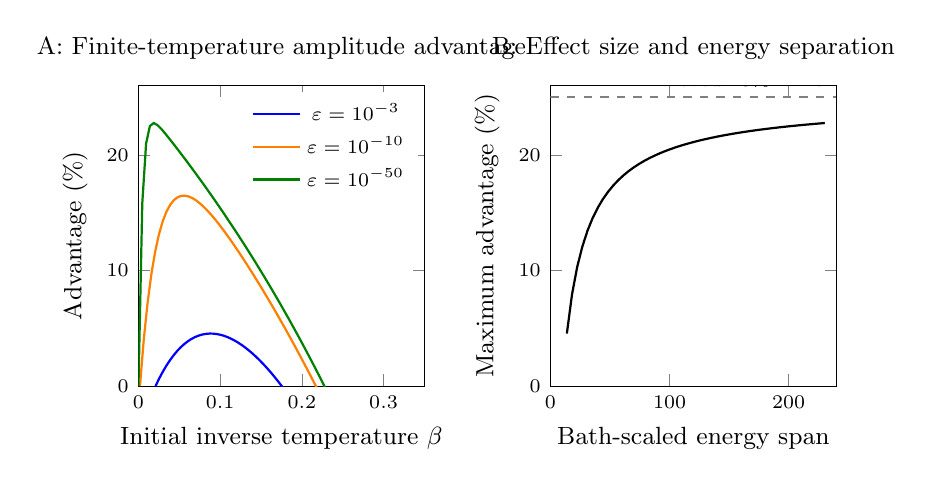
\begin{tikzpicture}
\begin{groupplot}[group style={group size=2 by 1,horizontal sep=1.6cm},width=.43\textwidth,height=5.4cm,tick label style={font=\scriptsize},label style={font=\small},title style={font=\small},ymin=0,ymax=26]
\nextgroupplot[title={A: Finite-temperature amplitude advantage},xmin=0,xmax=.35,xlabel={Initial inverse temperature $\beta$},ylabel={Advantage (\%)},legend style={font=\scriptsize,draw=none,at={(.98,.98)},anchor=north east}]
\addplot[blue,thick] coordinates {(0.02095685522,0) (0.02534409715,0.642018298331) (0.02973133908,1.22481549133) (0.03411858101,1.75128547588) (0.03850582294,2.22416754756) (0.04289306488,2.64605410908) (0.04728030681,3.01939802214) (0.05166754874,3.34651961566) (0.05605479067,3.62961336284) (0.0604420326,3.87075423963) (0.06482927453,4.07190377728) (0.06921651646,4.23491582097) (0.07360375839,4.36154200669) (0.07799100032,4.4534369682) (0.08237824225,4.5121632854) (0.08676548418,4.53919618556) (0.09115272611,4.53592800798) (0.09553996804,4.5036724429) (0.09992720997,4.44366855465) (0.1043144519,4.35708459905) (0.1087016938,4.24502164441) (0.1130889358,4.10851700546) (0.1174761777,3.94854749877) (0.1218634196,3.7660325284) (0.1262506616,3.56183700963) (0.1306379035,3.33677413874) (0.1350251454,3.09160801614) (0.1394123873,2.82705613011) (0.1437996293,2.54379170789) (0.1481868712,2.2424459406) (0.1525741131,1.92361008828) (0.1569613551,1.58783747093) (0.161348597,1.23564535121) (0.1657358389,0.867516714182) (0.1701230809,0.483901949222) (0.1745103228,0.085220438986) (0.1788975647,-0.32813793995) (0.1832848066,-0.75581140035) (0.1876720486,-1.19746490729) (0.1920592905,-1.65278891689) (0.1964465324,-2.12149818695) (0.2008337744,-2.60333065605) (0.2052210163,-3.09804638755) (0.2096082582,-3.60542657543) (0.2139955002,-4.12527260875) (0.2183827421,-4.65740519206) (0.222769984,-5.20166351879) (0.227157226,-5.75790449525) (0.2315444679,-6.32600201261) (0.2359317098,-6.90584626471) (0.2403189517,-7.49734310947) (0.2447061937,-8.10041347173) (0.2490934356,-8.71499278582) (0.2534806775,-9.34103047582) (0.2578679195,-9.97848947189) (0.2622551614,-10.6273457611) (0.2666424033,-11.2875879709) (0.2710296453,-11.9592169848) (0.2754168872,-12.6422455874) (0.2798041291,-13.3366981386) (0.284191371,-14.0426102761) (0.288578613,-14.7600286438) (0.2929658549,-15.4890106465) (0.2973530968,-16.2296242288) (0.3017403388,-16.9819476784) (0.3061275807,-17.7460694521) (0.3105148226,-18.5220880244) (0.3149020646,-19.3101117573) (0.3192893065,-20.1102587921) (0.3236765484,-20.9226569605) (0.3280637903,-21.747443717) (0.3324510323,-22.5847660896) (0.3368382742,-23.4347806509) (0.3412255161,-24.2976535075) (0.3456127581,-25.1735603077) (0.35,-26.0626862684) (0.35,-26.0626862684)};\addlegendentry{$\varepsilon=10^{-3}$}
\addplot[orange,thick] coordinates {(0.00188611697,0) (0.006527635411,3.99698440915) (0.01116915385,7.16556834959) (0.01581067229,9.66054209215) (0.02045219073,11.6076075858) (0.02509370917,13.1088443794) (0.02973522761,14.2471480614) (0.03437674605,15.0898344249) (0.03901826449,15.6915662231) (0.04365978293,16.0967298767) (0.04830130137,16.341365541) (0.05294281981,16.4547344938) (0.05758433825,16.4605920183) (0.0622258567,16.3782211324) (0.06686737514,16.2232721144) (0.07150889358,16.0084443177) (0.07615041202,15.7440399138) (0.08079193046,15.4384136245) (0.0854334489,15.0983379876) (0.09007496734,14.7293000227) (0.09471648578,14.3357421851) (0.09935800422,13.9212580707) (0.1039995227,13.4887513724) (0.1086410411,13.040564987) (0.1132825595,12.5785858805) (0.117924078,12.1043302613) (0.1225655964,11.6190127594) (0.1272071149,11.1236026142) (0.1318486333,10.6188693084) (0.1364901517,10.1054196305) (0.1411316702,9.58372777245) (0.1457731886,9.05415977062) (0.1504147071,8.51699335051) (0.1550562255,7.97243403763) (0.1596977439,7.4206282346) (0.1643392624,6.86167383318) (0.1689807808,6.29562882324) (0.1736222993,5.72251827396) (0.1782638177,5.14233999207) (0.1829053361,4.5550691047) (0.1875468546,3.96066176809) (0.192188373,3.35905816537) (0.1968298915,2.75018492624) (0.2014714099,2.13395707637) (0.2061129283,1.51027960394) (0.2107544468,0.879048714573) (0.2153959652,0.240152832283) (0.2200374837,-0.40652660653) (0.2246790021,-1.0611145281) (0.2293205205,-1.72374173433) (0.233962039,-2.39454452885) (0.2386035574,-3.07366443559) (0.2432450759,-3.76124799365) (0.2478865943,-4.45744661478) (0.2525281128,-5.16241649285) (0.2571696312,-5.87631855654) (0.2618111496,-6.59931845813) (0.2664526681,-7.33158659261) (0.2710941865,-8.07329814276) (0.275735705,-8.82463314627) (0.2803772234,-9.58577658214) (0.2850187418,-10.3569184739) (0.2896602603,-11.1382540081) (0.2943017787,-11.9299836658) (0.2989432972,-12.7323133678) (0.3035848156,-13.54545463) (0.308226334,-14.3696247314) (0.3128678525,-15.2050468918) (0.3175093709,-16.0519504601) (0.3221508894,-16.9105711136) (0.3267924078,-17.7811510669) (0.3314339262,-18.6639392916) (0.3360754447,-19.5591917465) (0.3407169631,-20.4671716188) (0.3453584816,-21.3881495764) (0.35,-22.3224040317) (0.35,-22.3224040317)};\addlegendentry{$\varepsilon=10^{-10}$}
\addplot[green!50!black,thick] coordinates {(7.54446788e-05,0) (0.004741105416,15.8069492769) (0.009406766154,20.977492026) (0.01407242689,22.4911503919) (0.01873808763,22.7458237542) (0.02340374837,22.5653325699) (0.0280694091,22.2326891674) (0.03273506984,21.8450953603) (0.03740073058,21.4359104387) (0.04206639132,21.0165570965) (0.04673205205,20.5909198259) (0.05139771279,20.1602921342) (0.05606337353,19.7250764075) (0.06072903427,19.2853679836) (0.06539469501,18.841155829) (0.07006035574,18.3923914761) (0.07472601648,17.9390126898) (0.07939167722,17.4809515772) (0.08405733796,17.0181373513) (0.08872299869,16.5504972562) (0.09338865943,16.0779568598) (0.09805432017,15.6004401286) (0.1027199809,15.1178694266) (0.1073856416,14.6301654877) (0.1120513024,14.1372473772) (0.1167169631,13.6390324496) (0.1213826239,13.1354363038) (0.1260482846,12.6263727363) (0.1307139453,12.111753693) (0.1353796061,11.5914892194) (0.1400452668,11.0654874087) (0.1447109275,10.5336543488) (0.1493765883,9.99589406739) (0.154042249,9.45210847492) (0.1587079098,8.90219730602) (0.1633735705,8.3460580588) (0.1680392312,7.78358593214) (0.172704892,7.21467376086) (0.1773705527,6.63921194866) (0.1820362134,6.05708839881) (0.1867018742,5.46818844241) (0.1913675349,4.8723947642) (0.1960331957,4.26958732574) (0.2006988564,3.659643286) (0.2053645171,3.042436919) (0.2100301779,2.41783952867) (0.2146958386,1.78571936062) (0.2193614993,1.1459415107) (0.2240271601,0.498367830374) (0.2286928208,-0.157143171462) (0.2333584816,-0.820736430161) (0.2380241423,-1.49256043079) (0.242689803,-2.17276731745) (0.2473554638,-2.86151300673) (0.2520211245,-3.55895730533) (0.2566867852,-4.26526403214) (0.261352446,-4.98060114502) (0.2660181067,-5.70514087225) (0.2706837675,-6.43905984923) (0.2753494282,-7.18253926027) (0.2800150889,-7.93576498604) (0.2846807497,-8.69892775667) (0.2893464104,-9.47222331103) (0.2940120711,-10.2558525621) (0.2986777319,-11.0500217693) (0.3033433926,-11.8549427173) (0.3080090534,-12.6708329022) (0.3126747141,-13.4979157259) (0.3173403748,-14.3364206973) (0.3220060356,-15.1865836427) (0.3266716963,-16.0486469249) (0.331337357,-16.9228596707) (0.3360030178,-17.8094780091) (0.3406686785,-18.7087653187) (0.3453343393,-19.6209924861) (0.35,-20.5464381754) (0.35,-20.5464381754)};\addlegendentry{$\varepsilon=10^{-50}$}
\nextgroupplot[title={B: Effect size and energy separation},xlabel={Bath-scaled energy span},ylabel={Maximum advantage (\%)},xmin=0,xmax=240]
\addplot[black,thick] coordinates {(13.81551056,4.54145185871) (18.14437053,7.92451781982) (22.47323051,10.2912735028) (26.80209048,12.0595950652) (31.13095046,13.4334078735) (35.45981043,14.5310277872) (39.78867041,15.4280316567) (44.11753038,16.1750178178) (48.44639036,16.8070126944) (52.77525033,17.3489639749) (57.10411031,17.8190929038) (61.43297028,18.2310064608) (65.76183026,18.5950668215) (70.09069023,18.9193030141) (74.41955021,19.2100326545) (78.74841018,19.4722953683) (83.07727016,19.7101610037) (87.40613013,19.9269527879) (91.7349901,20.1254115595) (96.06385008,20.3078184443) (100.3927101,20.4760877383) (104.72157,20.6318381105) (109.05043,20.776447809) (113.37929,20.911097915) (117.70815,21.03680656) (122.0370099,21.1544562381) (126.3658699,21.2648157873) (130.6947299,21.3685582178) (135.0235899,21.4662752758) (139.3524498,21.5584894214) (143.6813098,21.645663741) (148.0101698,21.7282101996) (152.3390298,21.8064965488) (156.6678897,21.8808521408) (160.9967497,21.9515728436) (165.3256097,22.0189252187) (169.6544697,22.0831500852) (173.9833296,22.144465574) (178.3121896,22.2030697563) (182.6410496,22.2591429126) (186.9699096,22.3128494994) (191.2987695,22.3643398605) (195.6276295,22.4137517184) (199.9564895,22.4612114812) (204.2853495,22.5068353885) (208.6142094,22.5507305211) (212.9430694,22.5929956919) (217.2719294,22.633722234) (221.6007893,22.6729947002) (225.9296493,22.7108914856) (230.2585093,22.7474853813) (230.2585093,22.7474853813)};
\addplot[gray,dashed] coordinates {(0,25)(240,25)};
\node[font=\scriptsize,anchor=south east] at (axis cs:237,25) {Proved $25\%$ limit};
\end{groupplot}
\end{tikzpicture}
\caption{The unperturbed family of Theorem~\ref{thm:quarterlimit}. Panel A plots $100[1-|b_2(\beta_h)|/|b_2(\beta)|]$ with finite $\beta_h=[\log(1/\varepsilon)]^{-2}$. Panel B follows its thermal maximum as the energy span $2\log(1/\varepsilon)$ grows. The substantial limiting advantage is accompanied by increasing energy separation; the plot does not claim practical cooling gains at modest spans. Curves and maxima use 80-digit arithmetic and illustrate the analytic theorem. The separate certified $22.617\%$ witness uses a different fixed hot preparation. The strict-triplet perturbation preserves the limiting result but is not plotted.}
\label{fig:quarter}
\end{figure}

\section{The sharp four-state amplitude bound under all triplet tests}
\label{sec:fulltripletbound}
The additional $F$ inequalities sharpen the contrast-cone bound from one
half to one quarter. The key restriction concerns the first three entries
of the slow eigenfunction, rather than monotonicity of all four entries.

\begin{lemma}[First-three arithmetic restriction]\label{lem:firstthreearithmetic}
Let a positive reversible four-state generator have distinct ordered
energies, a finite positive bath, a simple slow mode, and $F_{ijk}\leq0$,
$G_{ijk}\leq0$ on every original-rate triplet. Orient its slow left
eigenfunction by the nonnegative contrast coordinates of
Theorem~\ref{thm:orderedk}. Then
\[
w_1\geq w_2,\qquad w_1+w_2\geq2w_3,\qquad w_4\leq0.
\]
\end{lemma}
\begin{proof}
Write $q_i=\pi_i(\beta_b)$, $Q_j=\sum_{i\leq j}q_i$, and use the
unnormalized prefix contrasts $h^{(1)},h^{(2)},h^{(3)}$ from the contrast
theorem. Their coordinate generator is
\[
B=\operatorname{diag}(\eta_1,\eta_2,\eta_3)^{-1}H^\top D L H,
\quad H=(h^{(1)},h^{(2)},h^{(3)}),\quad D=\operatorname{diag}(q).
\]
It is diagonally similar to the symmetric Metzler contrast matrix. Its
Perron eigenvector $x$ can be chosen nonnegative and nonzero, and $w=Hx$.
Consequently $w_1-w_2=(Q_2/q_2)x_1\geq0$ and
$w_4=-(Q_3/q_4)x_3\leq0$. Put
\[
s=\frac{(q_1-q_2)q_3}{2q_2Q_3}>0.
\]
The remaining assertion is equivalent to $x_2\geq sx_1$, since
$w_1+w_2-2w_3=(2Q_3/q_3)(x_2-sx_1)$.

We first make a reset subtraction, which is used only in this proof and
does not alter the original triplet tests. The reduced conductances are
$k_{ij}=a_{ij}/q_i$. Their minimum is in the first row, by all the $G$
inequalities. Subtract
$k_* (q\mathbf1^\top-Q_4 I)$, where
$k_* =\min\{k_{12},k_{13},k_{14}\}$.
All resulting rates are nonnegative; their generator is reversible and
conservative, although it may be reducible. Every $F$ and $G$ is unchanged.
On the nonstationary contrast space this operation adds $k_*Q_4I$ to $B$,
so its eigenvectors, simplicity and eigenvalue ordering are unchanged.
The shifted largest contrast eigenvalue, denoted $\lambda$, is at most zero,
because the shifted full matrix remains a Markov generator. At least one
of the shifted downward rates $a_{12},a_{13},a_{14}$ is zero. All quantities
in the rest of this proof refer to this shifted generator.

If $x_1=0$, the assertion is immediate. Suppose $x_1>0$. Then
$\delta=\lambda-B_{33}>0$. To see strictness, symmetrize $B$: its largest
eigenvalue is at least its third diagonal entry. Equality would force the
third row and column of the positive semidefinite matrix
$\lambda I-\operatorname{diag}(\sqrt\eta)B
\operatorname{diag}(1/\sqrt\eta)$ to vanish. The third coordinate vector
would then be a Perron eigenvector. Simplicity would force $x_1=0$, a
contradiction. This also handles a zero shifted eigenvalue.

Eliminate $x_3$ from the eigenvector equations. The resulting two by two
matrix is
\[
\mathcal B_{ij}=B_{ij}+\frac{B_{i3}B_{3j}}{\delta},\qquad i,j\leq2.
\]
It has nonnegative off-diagonal entries and is diagonally symmetrizable.
The Schur complement of $\lambda I-B$ shows that $\lambda$ is its simple
largest eigenvalue, with eigenvector $(x_1,x_2)$.
Define
\[
C=B_{21}+s(B_{22}-B_{11})-s^2B_{12},\qquad
D_*=(B_{23}-sB_{13})(B_{31}+sB_{32}).
\]
Then
\[
\delta\{\mathcal B_{21}+s(\mathcal B_{22}-\mathcal B_{11})
-s^2\mathcal B_{12}\}=\delta C+D_*.
\]
A nonnegative value of this expression implies $x_2/x_1\geq s$. Indeed,
if the two off-diagonal entries of $\mathcal B$ are positive, its Perron
ratio is the unique positive root of the concave quadratic in braces,
viewed as a function of $s$. If those entries vanish, symmetrizability makes
both vanish. Since $x_1>0$ and the largest eigenvalue is simple, one then
has $x_2=0$ and $\mathcal B_{11}>\mathcal B_{22}$; the expression in braces
is strictly negative. Thus this exceptional case cannot occur when the
expression is nonnegative.

All $G$ inequalities give $B_{31},B_{32}\geq0$, and direct simplification gives
\[
B_{23}-sB_{13}
=\frac{Q_4}{2q_1q_2Q_3}
\{2a_{34}q_1q_2-a_{14}q_2q_3-a_{24}q_1q_3\}\geq0.
\]
Hence $D_*\geq0$. If $C\geq0$ the desired expression is already
nonnegative. If $C<0$, use $\lambda\leq0$ to obtain
\[
\delta C+D_*\geq-B_{33}C+D_*.
\]
It remains to prove that this last, eigenvalue-free expression is nonnegative.

For brevity write the shifted downward rates as
$(a,b,c,d,e,f)=(a_{12},a_{13},a_{14},a_{23},a_{24},a_{34})$ and define
\[
N=-2q_1q_2q_3F_{123}\geq0,\qquad
J=e q_1(2q_2+q_3)-c q_2(2q_1+q_3).
\]
Exact multiplication yields
\[
-B_{33}C+D_*=
\frac{Q_2Q_4}{4q_1q_2^2Q_3^2}\,T,
\quad
T=(c+e+f)N+q_4\{2ceq_3(q_1-q_2)+fJ\}.
\]
The prefactor is positive. Since at least one of $a,b,c$ is zero,
nonnegativity follows from these three exhaustive cases:
\begin{enumerate}
\item If $c=0$, then $J=e q_1(2q_2+q_3)\geq0$ and all terms of $T$
are nonnegative.
\item If $a=0$, $F_{124}\leq0$ gives
$c q_2(2q_1+q_4)\leq e q_1(2q_2+q_4)$.
The ratio $(2q_2+z)/(2q_1+z)$ strictly increases with $z$ and
$q_3>q_4$. It follows, without division by $c$ or $e$, that $J\geq0$.
Thus $T\geq0$.
\item If $b=0$, then
$N=2a q_2q_3(q_1-q_2)+d q_1q_3(2q_2+q_3)$.
If $c\leq e$, one has $J\geq0$. If $c>e$, the inequality
$F_{124}\leq0$ gives instead
\[
N+q_4J\geq
2q_1q_2(q_3-q_4)(c-e)+d q_1q_3(2q_2+q_3)\geq0.
\]
Now write
$T=(c+e)N+f(N+q_4J)+2ceq_3q_4(q_1-q_2)\geq0$.
\end{enumerate}
This proves $x_2\geq sx_1$ and completes the lemma, including equality
faces and every reducible reset-subtracted case.
\end{proof}

\begin{theorem}[Sharp quarter-amplitude bound]\label{thm:fulltripletbound}
Under the hypotheses of Lemma~\ref{lem:firstthreearithmetic}, for every
$0<\beta_h<\beta_c<\beta_b$,
\[
\frac{|b_2(\beta_c)|}{|b_2(\beta_h)|}<\frac43.
\]
Consequently every ordinary cooling amplitude advantage is strictly below
$25\%$. The bound is sharp as a supremum, by
Theorem~\ref{thm:quarterlimit}. The corresponding supremum of the
asymptotic relative-entropy advantage is $7/16$, and the time advance is
strictly below $\log(4/3)/|\lambda_2|$.
\end{theorem}
\begin{proof}
Let $m(\beta)$ be the conditional Gibbs expectation of $w$ on states
$1,2,3$. It is nondecreasing for $\beta\geq0$. To verify this directly,
shift $E_1=0$, put $a=E_2$, $b=E_3$, $t=e^{-\beta a}$ and
$y=e^{-\beta b}$, and use conditional probabilities
$(p_1,p_2,p_3)=(1,t,y)/(1+t+y)$. The first-three vector is a constant
plus
\[
u(1,-1,0)+v(1,1,-2),\qquad
u=(w_1-w_2)/2\geq0,\quad v=(w_1+w_2-2w_3)/6\geq0.
\]
Furthermore
\[
(p_1-p_2)'=\frac{2at+by-(b-a)ty}{(1+t+y)^2}>0,
\qquad (p_1+p_2-2p_3)'=-3p_3'>0.
\]
The first inequality uses $t\leq1$ and $b>a>0$; the second uses that
$E_3$ is the largest of the three energies. Thus $m$ is nondecreasing,
strictly unless the first three mode components coincide.

Let $P(\beta)=Z_3(\beta)/Z_4(\beta)$ be the Gibbs mass on the first three
states. It strictly increases with $\beta$, since the excluded state has
strictly higher energy. For finite positive $\beta$, $3/4<P(\beta)<1$.
Write $P_h=P(\beta_h)$, $P_c=P(\beta_c)$, and $r=P_c/P_h<4/3$.
The full overlap is $b_2=Pm+(1-P)w_4$. Therefore
\[
b_2(\beta_c)-r b_2(\beta_h)
=P_c\{m(\beta_c)-m(\beta_h)\}+(1-r)w_4\geq0.
\]
The contrast theorem ensures both overlaps are strictly negative on cooling,
so $|b_2(\beta_c)|\leq r|b_2(\beta_h)|<(4/3)|b_2(\beta_h)|$.
The relative-entropy and time-advance statements follow from their respective
quadratic and logarithmic dependence on the amplitude ratio. The existing
quarter-limit family proves sharpness; none of these suprema is attained at
finite parameters in the stated domain.
\end{proof}

\section{A finite-span necessary condition for a specified advantage}
\label{sec:finitespanamplitude}
The sharp quarter bound has a more restrictive form when the energy span
and the two preparation temperatures are specified.

\begin{corollary}[Finite-span cooling bound]
\label{cor:finitespanamplitude}
Under the full four-state hypotheses of
Theorem~\ref{thm:fulltripletbound}, put
\[
\Delta=E_4-E_1>0,\qquad
 d=(\beta_c-\beta_h)\Delta>0,\qquad
 p_{4,h}=\pi_4(\beta_h),
\]
for any finite $0<\beta_h<\beta_c<\beta_b$. The asymptotic
slow-amplitude advantage satisfies
\begin{equation}\label{eq:finitespanamplitude}
\mathcal A:=1-\frac{|b_2(\beta_h)|}{|b_2(\beta_c)|}
\leq p_{4,h}(1-e^{-d})
<\frac{1-e^{-d}}4
<\frac{1-e^{-\beta_b\Delta}}4.
\end{equation}
These bounds also hold when the ordering is ordinary and
$\mathcal A\leq0$.
Consequently, achieving $\mathcal A\geq g$ for a specified
$0<g<1/4$ requires
\[
(\beta_c-\beta_h)\Delta> -\log(1-4g),
\qquad p_{4,h}>g.
\]
In particular $\beta_b\Delta> -\log(1-4g)$ is necessary if the
preparation temperatures may be chosen freely on the cooling side.
These are necessary conditions only; no sufficiency or sharpness is
asserted for these finite-span bounds.
\end{corollary}
\begin{proof}
Write $P_3(\beta)=1-\pi_4(\beta)$. The proof of
Theorem~\ref{thm:fulltripletbound} established
\[
\frac{|b_2(\beta_c)|}{|b_2(\beta_h)|}
\leq\frac{P_3(\beta_c)}{P_3(\beta_h)}.
\]
Both overlaps are nonzero by the contrast theorem, so inversion gives
$\mathcal A\leq1-P_3(\beta_h)/P_3(\beta_c)$.
Shift the energy origin to $E_1=0$, leaving $E_4=\Delta$.
Then $Z_3(\beta_c)\leq Z_3(\beta_h)$ and
\[
\frac{\pi_4(\beta_c)}{P_3(\beta_c)}
=\frac{e^{-\beta_c\Delta}}{Z_3(\beta_c)}
\geq e^{-d}\frac{\pi_4(\beta_h)}{P_3(\beta_h)}.
\]
Multiplying by $P_3(\beta_h)$ gives
\[
\frac{P_3(\beta_h)}{P_3(\beta_c)}
\geq P_3(\beta_h)+e^{-d}p_{4,h},
\]
which proves the first bound. The highest-energy state has strictly
less than one-quarter Gibbs mass at finite positive $\beta_h$, so the
second inequality is strict. The last is strict because
$\beta_c-\beta_h<\beta_b$. Solving
$g<(1-e^{-d})/4$ gives the required dimensionless separation; also
$g\leq\mathcal A\leq p_{4,h}(1-e^{-d})<p_{4,h}$.
\end{proof}

For example, amplitude advantages of at least $10\%$, $20\%$, and
$24\%$ require, respectively,
\[
d>\log(5/3)\approx0.5108,\qquad
d>\log5\approx1.6094,\qquad
d>\log25\approx3.2189.
\]
They also require $p_{4,h}>0.10$, $0.20$, and $0.24$, respectively.
These are restrictions on initial inverse-temperature separation and
highest-state occupation, not guarantees that a generator satisfying
them exhibits an effect. The quantity $\mathcal A$ concerns the
asymptotic slow amplitude, not a finite-time distance or an absolute
relaxation-time reduction.

\subsection{An exact infinite-temperature endpoint criterion}
\label{sec:tripletendpoint}
The full triplet premise also removes the possible hidden interior cooling
interval: any anomaly begins at the high-temperature end of the Gibbs curve.
Only an endpoint derivative is needed to decide its existence.

\begin{corollary}[Cooling is decided by one endpoint covariance]
\label{cor:tripletendpoint}
Under the hypotheses and orientation of
Lemma~\ref{lem:firstthreearithmetic}, an ordinary asymptotic cooling effect
exists if and only if
\[
b_2'(0)<0,
\quad\text{equivalently}\quad
\operatorname{Cov}_{\mathrm{unif}}(w,E)>0.
\]
Here the uniform law is on all four states; $\beta=0$ is used only as an
analytic endpoint, not as an allowed witness preparation. If this condition
holds, there is exactly one finite positive stationary point of $b_2$.
It lies in $(0,\beta_b)$, and $|b_2|$ has its unique cooling maximum there.
The anomalous local ordering region is exactly $(0,\beta_{\rm turn})$.
If $b_2'(0)\geq0$, then $b_2'(\beta)>0$ for every finite $\beta>0$,
including when the endpoint derivative is zero, and no ordinary cooling
effect occurs. With a simple slow mode these conclusions apply to every
fixed norm asymptotically.
\end{corollary}
\begin{proof}
Write $b=b_2$. The contrast theorem gives $b<0$ on cooling and
$b'(\beta_b)>0$, as well as strict heating monotonicity. The derivative
at the bath is strictly positive directly: every prefix-contrast numerator
vanishes there with a strictly positive derivative, and the nonnegative
Perron coordinate vector is nonzero.

Put $C=w_3-w_4$. First suppose $C\geq0$. By the arithmetic restriction,
\[
m(0)=\frac{w_1+w_2+w_3}{3}\geq w_3\geq w_4,
\]
where $m$ is the conditional first-three Gibbs expectation from the sharp
bound. Since $m$ is nondecreasing, $b=Pm+(1-P)w_4$ gives
\[
b'=Pm'+P'(m-w_4)>0 \qquad (\beta\geq0).
\]
To justify strictness, if the first three components are not all equal,
the elementary contrast decomposition in the preceding proof gives
$m'>0$. Otherwise $m$ is constant, and nonconstancy of the full mode,
its zero bath mean and $w_4\leq0$ force $m>w_4$; then $P'>0$ supplies
strictness. Thus this case has no cooling anomaly.

Now suppose $C<0$. Use the derivative-curve representation
\eqref{eq:finitephi}: $b'=g\Phi$, where $g=\pi_1'>0$,
\[
\Phi(u)=A+Bu+C v(u),\qquad
u(\beta)\searrow-1 \text{ as }\beta\to\infty.
\]
The derivative-curve lemma makes $\Phi$ strictly concave in $u$.
It extends continuously to the two endpoints of
$[-1,u(0)]$, with
\[
\Phi(-1)=w_1-w_2\geq0,
\qquad \operatorname{sign}\Phi(u(0))=\operatorname{sign}b'(0).
\]
If $\Phi(u(0))\geq0$, strict concavity puts its value strictly above the
nonnegative chord at every interior point. Hence $b'(\beta)>0$ for every
finite $\beta>0$, even in the endpoint equality case.

If $\Phi(u(0))<0$, its positive value at the bath and its nonnegative
left endpoint imply that it has exactly one zero between $u(\beta_b)$
and $u(0)$. Indeed a concave function has an interval as its nonnegative
superlevel set; strict concavity and positivity at the bath rule out an
interior zero on the left-hand interval. On the right-hand interval the
slope of chords is decreasing, so after reaching zero the function cannot
return to nonnegative values. The zero is therefore unique, with negative
values to its right and positive values to its left. Since $u$ decreases
with $\beta$, $b'$ is negative for $0\leq\beta<\beta_{\rm turn}$ and
positive thereafter. The turning point lies strictly before the bath.
On cooling, $|b|=-b$, proving the stated maximum and anomalous interval.
Strict negativity persists at small finite positive inverse temperatures,
so the criterion supplies admissible finite witnesses.

Finally $b'(0)=-\operatorname{Cov}_{\mathrm{unif}}(w,E)$ by the fixed-mode
covariance identity. No interpretation of a stationary point alone is used.
\end{proof}

The covariance is explicitly
\[
\operatorname{Cov}_{\mathrm{unif}}(w,E)
=\frac14\sum_{i=1}^4w_iE_i
-\frac1{16}\Bigl(\sum_iw_i\Bigr)\Bigl(\sum_iE_i\Bigr).
\]
Thus within the triplet-failure family there is no need to scan the initial
cooling temperatures or solve an interior derivative equation merely to
decide existence. Section~\ref{sec:rateendpoint} gives an equivalent
evaluation using one cubic root and original-rate matrix products,
avoiding construction of the slow eigenvector. This is an asymptotic
criterion; it does not classify transient distance crossings.

\subsection{Exact classification when only one mode is faster}
\label{sec:fulltripletdegenerate}
The full triplet premise is especially restrictive when all but one of
the nonstationary modes share the slow rate. The resulting classification
holds in every dimension at least four and completely covers slow
spectral degeneracy in four states.

\begin{theorem}[A single faster mode must mix an adjacent pair]
\label{thm:tripletdegenerate}
Let $n\geq4$, and let $M$ be an irreducible reversible $n$-state generator
with distinct energy levels, positive finite bath temperature, and
$F_{ijk},G_{ijk}\leq0$ on every original-rate energy-ordered triplet.
Write $q=\pi(\beta_b)$, $D=\operatorname{diag}(q)$ and
$R=q\mathbf1^\top-I$. Suppose
\[
0>\lambda_2=\cdots=\lambda_{n-1}>\lambda_n.
\]
Then for exactly one $k\in\{1,\ldots,n-1\}$,
\[
M=\rho R+\delta J^{(k)},\qquad \rho>0,\quad\delta>0,
\]
where $J^{(k)}$ is supported on the adjacent pair $(k,k+1)$,
\[
J^{(k)}_{k,k+1}=\frac{q_k}{q_k+q_{k+1}},\qquad
J^{(k)}_{k+1,k}=\frac{q_{k+1}}{q_k+q_{k+1}},
\]
and its diagonal is set by zero column sums. Conversely, every such
matrix obeys all the triplet inequalities, with eigenvalues $0$,
$-\rho$ of multiplicity $n-2$, and $-\rho-\delta$.
If all nonzero eigenvalues coincide, then $M=\rho R$.

Every generator in these classes preserves stochastic order.
Consequently, for cooling or heating Gibbs preparations, the farther
preparation has at least as large a convex divergence from the bath at
every $t\geq0$. This holds for every convex function finite on positive
arguments; it is strict at finite times for strictly convex functions
and distinct preparations. In particular there is no ordinary or strong
asymptotic effect in KL or weighted Euclidean distance.
\end{theorem}
\begin{proof}
Use normalized weights $q_1>\cdots>q_n>0$.
Set $\rho=-\lambda_2$ and $\delta=\lambda_2-\lambda_n$.
The reversible spectral resolution gives
\[
M=\rho R-\frac{\delta}{N}Dzz^\top,
\qquad q^\top z=0,\qquad N=z^\top Dz>0,
\]
where $z$ is a real fast left eigenvector. Substitution of
$a_{ij}=\rho q_i-\delta q_i z_i z_j/N$ into the original tests gives
\begin{align*}
G_{ijk}&=-\frac{\delta q_j}{N}z_k(z_i-z_j),\\
F_{ijk}&=\frac{\delta}{N}\left\{
(q_i-q_j)z_i z_j-z_k\left[q_i z_i-q_j z_j
 +\frac{q_k}{2}(z_i-z_j)\right]\right\}.
\end{align*}
Thus $G\leq0$ means $z_k(z_i-z_j)\geq0$.
When $z_i=z_j=a$, the second identity is
$F_{ijk}=\delta(q_i-q_j)a(a-z_k)/N$; when $z_k=0$ it is
$F_{ijk}=\delta(q_i-q_j)z_i z_j/N$.

Let $m$ be the largest index with $z_m\ne0$ and orient $z_m>0$.
Zero bath mean excludes $m=1$.
If $m\geq4$, the tests $G_{ijm}\leq0$ order the entire prefix:
\[
z_1\geq z_2\geq\cdots\geq z_{m-1}.
\]
If some $i<j\leq m-2$ had $z_i>z_j$, the test
$G_{ij,m-1}\leq0$ would force $z_{m-1}\geq0$.
Every earlier entry would then be nonnegative, contradicting zero bath
mean because $z_m>0$ and all later entries vanish. Hence
\[
z_1=\cdots=z_{m-2}=a.
\]
Since $m-2\geq2$, $F_{12m}\leq0$ gives $0\leq a\leq z_m$.
Zero bath mean forces $z_{m-1}<0$, and $F_{12,m-1}\leq0$
then forces $a=0$. Therefore the support is exactly $(m-1,m)$.

If $m=3$, the condition $n\geq4$ supplies the zero component $z_4$.
The test $G_{123}\leq0$ gives $z_1\geq z_2$, and zero bath mean
forces $z_2<0$. Now $F_{124}\leq0$ gives $z_1\geq0$, whereas
$F_{134}\leq0$ gives $z_1\leq0$. Thus $z_1=0$, and the support
is exactly $(2,3)$. If $m=2$, zero bath mean immediately gives support
exactly $(1,2)$. This proves that only an adjacent pair can occur.

For support $(k,k+1)$ choose
$z_k=-1/q_k$, $z_{k+1}=1/q_{k+1}$.
Then $-Dzz^\top/N=J^{(k)}$ with the displayed rates. This proves
necessity and uniqueness of the pair. It also proves strict positivity
of all off-diagonal rates, even if only nonnegative rates were assumed.

For the converse put $d=\delta/(q_k+q_{k+1})$.
The only nonzero triplet tests are
\begin{align*}
F_{k,k+1,l}&=-(q_k-q_{k+1})d &&(l>k+1),\\
F_{i,k,k+1}&=-(q_k+q_{k+1}/2)d &&(i<k),\\
G_{i,k,k+1}&=-q_kd &&(i<k).
\end{align*}
They are all negative; every omitted test is zero.
The matrix $J^{(k)}$ has eigenvalue $-1$ on the right eigenvector
$Dz$ and vanishes on its $(n-1)$-dimensional kernel. The reset $R$
is $-I$ on the zero-sum probability-perturbation subspace. This proves
the spectrum. If all nonzero eigenvalues coincide, the reversible
spectral resolution directly gives $M=\rho R$.

For stochastic monotonicity, take adjacent differences
$d_i=f_{i+1}-f_i$ of functions. The backward reset generator induces
$-I$ on these differences. The difference matrix of $J^{(k)}$ has
only column $k$ nonzero: its diagonal entry is $-1$, its entry in
row $k-1$, when present, is $q_{k+1}/(q_k+q_{k+1})$, and its entry
in row $k+1$, when present, is $q_k/(q_k+q_{k+1})$.
Thus the difference generator is Metzler. The earlier reversible
stochastic-order argument gives all-time convex-divergence ordering.
Strict convexity makes its supporting-line inequality strict for
unequal evolved distributions, which remain unequal at finite times
because $e^{tM}$ is invertible. This argument never selects a scalar
vector from the repeated slow eigenspace. The strong-effect exclusion
also follows directly from the earlier all-$G$ projection theorem.
\end{proof}

\begin{corollary}[The complete four-state degenerate boundary]
Under the full four-state triplet premise, a double slow eigenvalue
forces reset plus one adjacent-pair mixing term, and a triple slow
eigenvalue forces pure reset. Both cases have all-time convex-divergence
ordering. In particular every ordinary asymptotic cooling counterexample in KL
or weighted Euclidean distance has a simple slow eigenvalue. Strict failure of all eight linear tests
also forces spectral simplicity at the slow rate, since the classified
degenerate generators have several triplet equalities.
\end{corollary}

The inequalities $F,G\leq0$ are the primary hypotheses if zero
rates are initially allowed; they agree with the original branchwise
predicate for positive rates. This avoids defining $\kappa$ by division
by a possibly zero rate. The classification then implies positivity.

The reset-plus-pair family itself is prior work. Section II of
\href{https://arxiv.org/html/2609.09988v1}{Gelbwaser-Klimovsky,
\emph{Efficient protocol for the Markovian Mpemba effect in $N$-level
systems}, arXiv:2609.09988v1, 9 September 2026} introduces the single-pair
states-deviation protocol (SPSD). Our $\delta>0$ adjacent-pair family is
its positive-deviation case, with
$\Delta=\delta/[\rho(q_k+q_{k+1})]$. That source already shows that
positive pair deviation can activate the triplet test only when a level
lies strictly between the pair. The necessity proved here is a converse
classification: under the one-fast-mode spectrum and all triplet
failures, every admissible generator must belong to that adjacent-pair
family. The all-time divergence conclusion is an application of the
established stochastic-order method, not a new construction or principle.

The restriction $n\geq4$ is essential for the rank-one classification.
For $n=3$, take $q=(3/5,3/10,1/10)$, $z=(1,2,-12)$, and
$M=R-Dzz^\top/(z^\top Dz)$. All rates are positive, its spectrum is
$0,-1,-2$, and $F_{123}=0$, $G_{123}=-2/9$, but the fast mode uses
all three states. There is no repeated slow eigenvalue in that dimension;
the example pinpoints why an additional triplet is needed in the proof.
For $n>4$, the theorem concerns slow multiplicity exactly $n-2$ (or
$n-1$ for reset). It does not classify smaller repeated slow eigenspaces
with two or more distinct faster modes. No publication-priority claim
is made for this classification.

Exact rank-one identities and general pair formulas are audited by
\path{research/one_fast_mode_certificate.py}. The script additionally
checks explicit symbolic matrices in dimensions four through eight,
including their projector identities, spectra, triplet tables and
Metzler difference matrices; the arbitrary-dimensional statement is
proved by the support argument above, not inferred from those checks.

The restriction on multiplicity matters structurally. A five-state
counterexample to extending the monotonicity conclusion to every repeated
slow space has $q=(24,12,4,2,1)/43$ and spectrum
$0,-1,-1,-2,-3$. It obeys all $F,G\leq0$, yet its adjacent-difference
matrix has entry $K_{21}=-14/27$. The exact construction is given in
\path{research/five_state_degenerate_nonmonotone.txt} and checked by its
companion script. This rules out that stronger structural inference;
it does not by itself exhibit a thermal divergence reversal.

\subsection{A scalar rate test without computing a slow eigenvector}
\label{sec:rateendpoint}
The endpoint criterion can be evaluated from the generator and one root
of a cubic. This uses the classical polynomial formula for a spectral
projector; the point is an explicit implementation of the preceding
problem-specific criterion, not a new projector construction.

Let $q=\pi(\beta_b)$, $D=\operatorname{diag}(q)$, and put
\[
a=\tfrac14\mathbf1-q,\qquad
d=-\tfrac14(E-\bar E\mathbf1),\qquad
\bar E=\tfrac14\sum_i E_i,\qquad h=D^{-1}a.
\]
Thus $a$ is the infinite-temperature displacement and $d=\pi'(0)$.
Define $\tau=\operatorname{tr}M$,
$\sigma=[(\operatorname{tr}M)^2-\operatorname{tr}(M^2)]/2$ and
$A_j=h^\top M^j d$ for $j=0,1,2$. The scalar polynomial
\[
\mathcal R(x)=A_0x^2+(A_1-\tau A_0)x
                  +A_2-\tau A_1+\sigma A_0
\]
has degree at most two. Let
$p(x)=\det(xI-M)/x$ and let $r$ be its largest root.

\begin{corollary}[Rate evaluation of the triplet endpoint test]
\label{cor:rateendpoint}
For a positive reversible four-state generator satisfying all original
triplet failures, if $r$ is simple, ordinary asymptotic cooling occurs
if and only if $\mathcal R(r)>0$. Equality means absence.
If the largest nonzero root is repeated, cooling is absent by
Theorem~\ref{thm:tripletdegenerate}. Thus the full-premise decision
requires a cubic root and a scalar quadratic evaluation, with no
choice or numerical normalization of a slow eigenvector.
\end{corollary}
\begin{proof}
Write the other two roots as $s,t$, permitting $s=t<r$.
On the invariant zero-sum subspace the spectral projector onto $r$ is
\[
P_r=\frac{(M-sI)(M-tI)}{(r-s)(r-t)}
=\frac{M^2-(\tau-r)M+(\sigma-\tau r+r^2)I}{p'(r)}.
\]
This identity is asserted on that subspace, not on the stationary
direction. Reversibility ensures diagonalizability even if $s=t$.
Since $d$ has zero sum, it follows that
$h^\top P_r d=\mathcal R(r)/p'(r)$.
For any nonzero left slow eigenvector $w$, detailed balance gives
\[
P_r=\frac{Dw w^\top}{w^\top Dw},\qquad
\frac{\mathcal R(r)}{p'(r)}
=\frac{(w^\top a)(w^\top d)}{w^\top Dw}
=\frac{b(0)b'(0)}{w^\top Dw}.
\]
Here $w^\top q=0$, so $b(0)=w^\top a$. Orienting the mode by
the contrast theorem makes $b(0)<0$. Corollary~\ref{cor:tripletendpoint}
therefore makes the product positive exactly when cooling occurs.
Finally $p'(r)=(r-s)(r-t)>0$, proving the sign rule, including equality.
\end{proof}

All quantities except the single cubic root are explicit matrix products
of the original rates, bath weights, and energies. The test still uses
global spectral information through $r$; it is not a new local triplet
test. For rational bath weights and commensurate energies, the common
positive energy unit can be removed and the remaining sign can be
decided by ordered algebraic arithmetic. For arbitrary real energies,
floating evaluation near zero does not settle exact equality. This
corollary concerns existence of an asymptotic effect, not every transient
crossing for a specified distance.

\subsection{Exact rational-input classification without commensurate energies}
\label{sec:rationallogendpoint}
Within the full triplet-failure family, the endpoint criterion admits a
terminating exact decision procedure even when the energy gaps are
incommensurate. The additional ingredient is Baker's linear-independence
theorem for logarithms, rather than a polynomial substitution for the whole
Gibbs curve. This is a consequence of an established transcendence theorem;
no new number-theoretic independence claim is made.

\begin{theorem}[Rational-input endpoint decision]
\label{thm:rationallogendpoint}
Consider a positive reversible four-state generator with rational entries,
distinct ordered Gibbs bath weights and positive finite bath temperature.
Suppose all original triplet predicates fail. Ordinary asymptotic cooling
in relative entropy or weighted Euclidean distance can be decided by a
terminating exact procedure using rational arithmetic,
integer factorization, real algebraic root isolation and rational logarithm
enclosures. Commensurate energy gaps are not required. A repeated slow
eigenvalue is handled by the preceding degenerate-boundary classification,
which excludes an effect in these distances. When the slow mode is simple,
the same decision applies asymptotically to every fixed norm.
The procedure concerns this full-triplet family;
it is not a classifier for arbitrary unconstrained rational generators or
for transient distance crossings.
\end{theorem}
\begin{proof}
The unique normalized stationary law $q$ is rational, since it solves a
rational linear system. Equivalently one may supply rational ordered bath
weights and rational downward rates, construct the reverse rates by detailed
balance, and check the hypotheses exactly. In bath energy units take
$E_i=-\log q_i$; an additive energy shift does not affect the criterion.
All logarithms below are the real logarithms of positive numbers.

Let $r$ be the largest root of the rational nonzero characteristic cubic
$p(x)=\det(xI-M)/x$. Determine its multiplicity exactly. If it is repeated,
the full-triplet degeneracy theorem returns absence of an effect. Otherwise
write
\[
\tau=\operatorname{tr}M,\qquad
\sigma=\frac{\tau^2-\operatorname{tr}(M^2)}2,\qquad
K_r=M^2-(\tau-r)M+(\sigma-\tau r+r^2)I.
\]
Define the rational vectors and matrix
\[
a=\tfrac14\mathbf1-q,\qquad h=D^{-1}a,\qquad
T=I-\tfrac14\mathbf1\mathbf1^\top,
\quad D=\operatorname{diag}(q),
\]
and the row vector
\[
c^\top=\tfrac14 h^\top K_r T\in\mathbb Q(r)^{1\times4}.
\]
The endpoint scalar from the spectral-projector test is
\begin{equation}\label{eq:rationalprimelog}
\mathcal R(r)=\sum_{i=1}^4c_i\log q_i.
\end{equation}
Indeed $\pi'(0)=\tfrac14T(\log q_i)_i$, and on the zero-sum probability
subspace the slow spectral projector is $K_r/p'(r)$. Since $\pi'(0)$
has zero sum, this suffices even though the polynomial need not annihilate
the stationary direction on the full space. For an oriented slow left mode
$w$, the projector identity gives
\[
\frac{\mathcal R(r)}{p'(r)}
=\frac{(w^\top a)(w^\top\pi'(0))}{w^\top Dw}.
\]
Here $p'(r)>0$ for a simple largest nonzero root, including when the two
faster roots coincide, and $w^\top a=b_2(0)<0$ by the contrast theorem.
Thus the single-endpoint criterion says cooling occurs exactly when
$\mathcal R(r)>0$; equality means absence, not an undecided threshold.

Factor the numerators and denominators of the four positive rationals $q_i$.
Let $\mathcal P$ be the resulting finite set of primes and write
\[
q_i=\prod_{\ell\in\mathcal P}\ell^{v_{\ell i}},
\qquad v_{\ell i}\in\mathbb Z.
\]
Then
\[
\mathcal R(r)=\sum_{\ell\in\mathcal P}\gamma_\ell\log\ell,
\qquad
\gamma_\ell=\sum_i v_{\ell i}c_i\in\mathbb Q(r).
\]
Each $\gamma_\ell$ has an exact zero test in the real algebraic field
specified by the isolated root $r$.

The precise external theorem needed is the following form of Baker's result:
if logarithms of nonzero algebraic numbers, together with $2\pi i$, are
linearly independent over $\mathbb Q$, those logarithms are linearly
independent over $\overline{\mathbb Q}$.
This is stated in the opening paragraph of
\href{https://doi.org/10.1112/S0025579300008068}{A.~Baker,
\emph{Linear forms in the logarithms of algebraic numbers (II)},
Mathematika 14 (1967), 102--107}, referring to the original
\href{https://doi.org/10.1112/S0025579300003971}{1966 paper,
Mathematika 13, 204--216}.
For distinct positive primes, rational independence of their real logarithms
follows from unique prime factorization: clear the denominators of a rational
relation and exponentiate. Adjoining $2\pi i$ preserves that independence
because all the prime logarithms are real. Baker's theorem therefore gives
\[
\mathcal R(r)=0\quad\Longleftrightarrow\quad
\gamma_\ell=0\ \text{for every }\ell\in\mathcal P.
\]
This is linear independence over algebraic coefficients, not algebraic
independence of the logarithms. There is no branch ambiguity: only real
logs of primes greater than one are used. A rational factor equal to one
has empty factorization and contributes zero, so $\log1$ is never included
in the independent set.

If every coefficient vanishes, return equality and absence. Otherwise the
sum is a nonzero real number. Refine the rational isolating interval for
$r$, evaluate the algebraic coefficients by directed rational interval
arithmetic, and enclose each logarithm by a convergent rational series.
For example, for a prime $\ell$ put $z=(\ell-1)/(\ell+1)\in(0,1)$.
The partial sum and a valid tail bound are
\[
L_N=2\sum_{j=0}^{N}\frac{z^{2j+1}}{2j+1},\qquad
0<\log\ell-L_N\leq
\frac{2z^{2N+3}}{(2N+3)(1-z^2)}.
\]
All quantities on the right are rational and the bound tends to zero.
Refining all intervals produces an enclosure of $\mathcal R(r)$ whose
width tends to zero. Its nonvanishing guarantees that eventually the
enclosure excludes zero, deciding its sign. No unproved transcendental
equality oracle or floating-point tolerance enters the decision.
\end{proof}

The theorem establishes termination, not a practical complexity bound.
Integer factorization and very small nonzero logarithmic forms can be
expensive; no uniform precision or runtime promise is made. It also does
not remove the full-generator spectral dependence: isolating the one slow
cubic root remains necessary, although a full slow eigenvector and a scan
of initial temperatures are avoided. For arbitrary nonrational input data,
the analytic scalar criterion remains valid but this rational-input
termination argument does not apply.

The implementation is \path{research/exact_rational_triplet_classifier.py}.
It checks the full premise exactly, factors the supplied rational weights,
and uses the selected real algebraic embedding throughout. Range reduction
to logarithms of numbers between one and two accelerates the rational
series. An optional resource limit returns an unresolved result, never
absence. With no such limit the theorem gives termination. The original
counterexample, whose energy gaps are not all commensurate, is classified
as cooling by an exact positive endpoint enclosure. An independent
implementation audit includes commensurate comparisons with the Sturm
classifier, scale invariance, degenerate cases and invalid-input rejection.

\section{Counterexamples in every higher dimension}\label{sec:extension}
The failure is not restricted to exactly four states. A fast, high-energy
state can be added without repairing any of the triplet tests.

\begin{theorem}[Dimension extension]\label{thm:extension}
Suppose an $n$-state positive reversible generator, with distinct energies
and a positive finite bath, has a simple slow mode and a strict ordinary
cooling witness at two finite positive initial temperatures. Suppose every
original-rate triplet predicate fails. There is an $(n+1)$-state positive
reversible system with the same properties, retaining every original
off-diagonal rate. If all original $F,G$ inequalities are strict, every
inequality in the extension is strict as well. Consequently, counterexamples
form nonempty open sets for every state count $n\geq4$.
\end{theorem}
\begin{proof}
Use units $\beta_b=1$ and unnormalized bath weights $q_i=e^{-E_i}$.
Choose $A>0$ so large that $-nA$ lies strictly below every original nonzero
eigenvalue. Add a new highest state of weight $\epsilon=e^{-E_{n+1}}$,
with downward rates $a_{i,n+1}=A$ for every $i\leq n$ and reverse rates
$a_{n+1,i}=A\epsilon/q_i$. Recompute the diagonal to conserve probability.
All rates are positive and detailed balance holds. Original triplet tests
are unchanged. In a new triplet $i<j<n+1$, writing
$t=e^{-(E_j-E_i)}<1$, $u=e^{-(E_{n+1}-E_j)}>0$, and $C=a_{ij}>0$, one has
\[
G=A(t-1)<0,\qquad F=-(1-t)(C+Au/2)<0.
\]
Thus every added triplet fails strictly.

As $\epsilon\downarrow0$, the full generator tends to
\[
\begin{pmatrix}M&A\mathbf1\\0&-nA\end{pmatrix}.
\]
Its spectrum is the original spectrum together with $-nA$. The original
slow eigenvalue remains simple and separated. Its left eigenvector extends
from $w$ to
\[
\left(w,\frac{A\sum_{i=1}^n w_i}{\lambda_2+nA}\right).
\]
The denominator is nonzero by the choice of $A$. Ordinary finite-dimensional
perturbation theory for a simple eigenvalue now supplies a continuously
normalized slow eigenvector for sufficiently small positive $\epsilon$,
with a spectral gap bounded away from zero. This argument uses the generator
directly; it does not symmetrize at the singular limiting bath weight.

For either fixed initial inverse temperature $\beta>0$, the new Gibbs
weight is $\epsilon^\beta\to0$, so its preparation converges to the old
Gibbs vector with a zero extra coordinate. The two slow overlaps therefore
converge to the original overlaps. Their strict inequality persists for
sufficiently small positive $\epsilon$. Every energy is then finite and
distinct. Induction extends the four-state counterexample to every larger
dimension. Starting from the strict four-state example, all triplet margins,
rate positivity, spectral simplicity and the overlap inequality are strict;
continuity gives an open neighborhood at each finite extension in the
energy/downward-rate parametrization of reversible systems.
\end{proof}

The construction adds rapidly emptying, initially weakly populated high-energy
states. It establishes dimensional persistence, not an enhancement of the
effect or a claim that the added states are experimentally useful. In
particular, the finite positive witness temperatures must be fixed before
taking the high-energy limit; the argument would not apply to a preparation
at exactly infinite temperature.

The standard-library checker \texttt{five\_state\_extension\_certificate.py}
adds $E_5=9000\log10$ to the primary four-state witness, with $A=1000$.
It verifies all ten original Boolean triplet predicates, all twenty positive
rates, detailed balance and column conservation. Exact rational inertia
places the new fast eigenvalue in $(-4001,-3999)$ and preserves the original
three spectral brackets. A weighted residual estimate controls the original
four eigenvector coordinates; the new row equation controls the fifth without
dividing by its extremely small bath weight. The same finite preparations
$\beta_h=1/1000$, $\beta_c=1/100$ retain a rigorously certified overlap
advantage greater than $10^{-4}$. The fifth state's thermal weights are
exactly $10^{-9}$ and $10^{-90}$ at those preparations.

\section{Hidden cooling advantages approaching unity with dimension}
\label{sec:highdimamplitude}
The sharp four-state bound does not give a dimension-independent bound.
Cloning the high-energy state produces an increasingly large normalization
change along the initial Gibbs curve, while retaining a uniformly isolated
slow relaxation mode.

\begin{theorem}[A dimension-dependent achievable advantage]
\label{thm:highdimamplitude}
For every integer $n\geq4$ there is a family of strictly positive,
reversible $n$-state generators at bath inverse temperature one, with
all energies distinct and all original $F_{ijk},G_{ijk}<0$, such that
finite $0<\beta_h<\beta_c<1$ satisfy
\[
1-\frac{|b_2(\beta_h)|}{|b_2(\beta_c)|}
\longrightarrow 1-\frac3n.
\]
The slow eigenvalue tends to $-3$ and its separation from the next mode
is greater than $1/4$ for all sufficiently small family parameters.
The corresponding leading asymptotic KL advantage tends to $1-9/n^2$.
Consequently no dimension-independent upper bound less than one can
hold for these amplitude or leading KL advantages under the full
triplet premise. Sharpness is asserted only for $n=4$, by the preceding
four-state theorem; no matching upper bound is claimed for $n>4$.
\end{theorem}
\begin{proof}
Fix $n$, put $m=n-3$, and choose strictly decreasing clone weights
\[
r_j=\frac{2^{m-j}}{2^m-1},\qquad j=1,\ldots,m,\qquad \sum_jr_j=1.
\]
Start with the quarter-limit family $M_\varepsilon$, its normalized bath
weights $q_i$, and its left slow vector $w$ from
Theorem~\ref{thm:quarterlimit}. Replace its fourth state by $m$ states
$c_1,\ldots,c_m$ with weights $q_4r_j$. Equivalently the unnormalized
bath weights are
\[
\widehat q^{(n)}=(1,1-\varepsilon/3,3/5,
                  \varepsilon^2r_1,\ldots,\varepsilon^2r_m).
\]
Their sum remains the four-state partition function. For small positive
$\varepsilon$ they give $n$ distinct ordered energies
$E_i=-\log\widehat q_i^{(n)}$.

Keep the original rates among the first three states. From each clone to
low state $i\leq3$ set $a_{i,c_j}=a_{i4}$, and in the reverse direction
set $a_{c_j,i}=r_j a_{4i}$. Within the clone block use conditional reset
at rate four: $a_{c_j,c_k}=4r_j$ for $j\ne k$.
Set all diagonals by conservation, giving a generator $\overline M$.
All rates are positive and detailed balance is immediate.
Lumping the clone probabilities exactly recovers $M_\varepsilon$.
The additional $(m-1)$-dimensional subspace consists of probability
perturbations supported on the clones whose sum is zero. On this
subspace the generator is scalar, with eigenvalue
\[
-4-\sum_{i=1}^3a_{i4}<-4.
\]
Thus $\overline M$ retains the simple slow eigenvalue $-3$, gap exceeding
$1/3$, and left eigenvector
\[
\overline w=(1,-4/5,w_3,-\varepsilon,\ldots,-\varepsilon).
\]
It has zero bath mean and weighted norm at most one for small
$\varepsilon$.

Here are all the original-rate triplet checks before a small repair.
Triplets in the first three states are unchanged. For two low states
$i<j\leq3$ and a clone $c_l$,
\[
G_{ijc_l}=G_{ij4},\qquad
F_{ijc_l}=F_{ij4}+
 \frac{(r_l-1)q_4}{2q_j}G_{ij4}.
\]
For one low state $i$ and two clones $c_j<c_k$,
\[
G_{ic_jc_k}=r_j(a_{4i}-4),\qquad
F_{ic_jc_k}=(r_j+r_k/2)(a_{4i}-4).
\]
All-clone triplets have $F=G=0$.
The original rates satisfy $0<a_{i4}<2$ throughout
$0<\varepsilon\leq1/30$. This bound is proved by three exact Bernstein
checks on the rational generator. Their finite limits are
\[
(a_{14},a_{24},a_{34})\longrightarrow(220,220,132)/169.
\]
Consequently $a_{4i}=a_{i4}q_4/q_i\leq(10/3)\varepsilon^2<4$,
so the one-low triplets are strictly negative. For the two-low/clone
triplets, $G_{ij4}\leq0$ and $-G_{ij4}\leq a_{j4}<2$, while
$q_4/q_j\leq(5/3)\varepsilon^2$. Thus the possible positive defect in
$F$ is at most $(5/3)\varepsilon^2$. Every $G$ is already nonpositive.

Define an auxiliary generator $H$ at the new bath weights. On the first
three states its reduced conductances are
$k_{12}=100,k_{13}=10,k_{23}=11$. Between low state $i$ and any clone
use $k_{i,c_j}=i$; among ordered clones use constant downward rate four,
with reverse rates fixed by detailed balance. All its tests are strictly
negative throughout $0<\varepsilon\leq1/30$.
The first-three tests are exactly those of the certified auxiliary
generator in the quarter-limit construction. Write
$Q=13/5-\varepsilon/3+\varepsilon^2$ for the unchanged partition sum.
For low pairs $12,13,23$ and clone $c_l$, the $F$ values of $H$ are
\[
\frac{-1-98\varepsilon/3-\varepsilon^2r_l/2}{Q},\qquad
\frac{-24/5-\varepsilon^2r_l}{Q},\qquad
\frac{-21/5+3\varepsilon-\varepsilon^2r_l/2}{Q}.
\]
Each is at most $-1/3$ on the interval, and the $G$ values are
strictly negative. For one low state $i$ and clones $j<k$ the tests are
\[
G=i q_{c_j}-4<0,\qquad F=G(1+q_{c_k}/(2q_{c_j}))<0.
\]
For three clones they are $G=4(t-1)<0$ and
$F=4(t-1)(1+u/2)<0$, since the $r_j$ are distinct and ordered.

Now put $\widetilde M=\overline M+6\varepsilon^2H$.
Linearity makes every $G$ strict. In two-low/clone triplets,
\[
F(\widetilde M)\leq(5/3)\varepsilon^2
                 -6\varepsilon^2/3=-\varepsilon^2/3<0.
\]
All other $F$ tests are already negative or acquire a strict negative
contribution from $H$. Thus all tests are strict on the entire
interval $0<\varepsilon\leq1/30$.

The repair does not spoil the spectrum or limiting overlaps. Let
$D_n=\operatorname{diag}(q^{(n)})$.
The symmetric matrix $D_n^{-1/2}HD_n^{1/2}$ has operator norm at most
\[
C_n=2\{103+4(m-1)\}.
\]
Indeed all rates leaving a low state sum to at most $103$, and those
leaving a clone sum to at most $3+4(m-1)$; each upward internal clone
rate is at most its downward rate four. Gershgorin applied to the
column generator and reversibility place its eigenvalues in
$[-C_n,0]$. This argument avoids any assumption of uniformly bounded
reduced conductances inside the increasingly rare clone block.
Weyl's inequality gives slow separation at least
$1/3-12C_n\varepsilon^2>1/4$ for sufficiently small $\varepsilon$.
The isolated eigenvector perturbation estimate in the quarter-limit
proof gives, with consistent orientation and equal weighted norm,
\[
\|\widetilde w-\overline w\|_{q^{(n)}}=O_n(\varepsilon^2).
\]
Since $q_i^{(n)}\geq r_m\varepsilon^2/3$ for small $\varepsilon$,
\[
\max_i|\widetilde w_i-\overline w_i|=O_n(\varepsilon).
\]
Every thermal overlap changes by at most this quantity, uniformly in
initial inverse temperature. The constants may depend on the fixed
integer $n$; no joint limit with $n$ and $\varepsilon$ is used.

Finally put $L=\log(1/\varepsilon)$ and choose
$\beta_h=L^{-2}$, $\beta_c=L^{-1/2}$. At $\beta_h$ every unnormalized
Gibbs weight tends to one. At $\beta_c$ each clone weight
$\exp(-2\sqrt L)r_j^{1/\sqrt L}$ tends to zero, while the first three
weights tend to one. Since the first three limiting slow components
sum to $-2/15$ and all clone components tend to zero,
\[
b_h\longrightarrow-\frac{2}{15n},\qquad
b_c\longrightarrow-\frac2{45}.
\]
The repair error tends to zero, so the ratio tends to $3/n$.
Both limiting overlaps are nonzero for each fixed $n$, and $3/n<1$,
which proves an admissible strict cooling witness for sufficiently
small positive $\varepsilon$. The leading KL ratio is the square of
the amplitude ratio, giving the stated KL advantage. Letting $n$
grow after taking these fixed-dimensional limits proves the absence
of a dimension-independent bound below one.
\end{proof}

The checker \path{research/high_dimension_amplitude_certificate.py}
records the exact cloning identities and six Bernstein sign certificates.
It also constructs the rational five-state member with
$\varepsilon=1/1000$ and clone weights $(2/3,1/3)$, verifies every strict
triplet test, positivity, conservation and detailed balance, and certifies
a perturbed slow gap of at least $124037/375000>1/4$.
This illustrative finite member verifies the generator construction; it
is not presented as a separately interval-certified thermal witness.
The all-dimensional thermal advantage is established by the limit proof.

There is also a separately certified finite five-state thermal witness.
For $m=2$, every outgoing rate sum of $H$ is at most $100$, so its
symmetric operator norm is at most $200$. Write
$\eta=1200\varepsilon^2$ for the perturbation bound. For
$\varepsilon\leq1/200$, the gap stays above
$1/3-2\eta\geq41/150>1/4$, and the oriented eigenvector estimate gives
\[
\|\widetilde w-\overline w\|_{q^{(5)}}
\leq\frac{\sqrt2\,\eta}{1/3-\eta}<6000\varepsilon^2.
\]
The normalization is the same weighted norm as $\overline w$, which is
at most one. Since the smallest normalized bath weight is at least
$\varepsilon^2/9$, every component and thermal overlap changes by less
than $18000\varepsilon$.
At $\varepsilon=10^{-50}$, $\beta_h=1/10000$ and $\beta_c=1/50$,
integer-power root bounds, combined with that error, enclose the repaired
amplitude advantage between $37.6778168708\%$ and $37.6778168731\%$.
The exact rational endpoints and reproducible computation are in
\path{research/five_state_large_advantage_certificate.py} and its JSON
receipt. This witness exceeds the four-state supremum. Its very large
energy span remains a mathematical construction, not evidence of a
practical cooling protocol.

\section{A precise reduction of the remaining dimensional bound}
\label{sec:highdimboundreduction}
The construction above and the contrast bound leave a specific structural
question. The next proposition isolates a sufficient additional inequality;
it does not assert that all the original $F$ tests force that inequality
in arbitrary dimension.

\begin{proposition}[Conditional three-state reduction]
\label{prop:highdimboundreduction}
Let $n\geq4$, let the energies be distinct and ordered, and let a positive
reversible generator at $0<\beta_b<\infty$ have a simple slow mode.
Suppose every original $G_{ijk}\leq0$. Orient the slow left eigenfunction
$w$ by its nonnegative weighted-prefix contrast coordinates, as in
Theorem~\ref{thm:orderedk}. If additionally
\begin{equation}\label{eq:highdimarithmetic}
w_1+w_2\geq2w_3,
\end{equation}
then every finite cooling pair $0<\beta_h<\beta_c<\beta_b$ satisfies
\[
\frac{|b_2(\beta_c)|}{|b_2(\beta_h)|}<\frac n3.
\]
In particular its amplitude advantage is strictly below $1-3/n$.
\end{proposition}
\begin{proof}
Write $q_i=\pi_i(\beta_b)$, $Q_k=\sum_{i\leq k}q_i$, and
\[
h^{(k)}_i=
\begin{cases}
1,&i\leq k,\\
-Q_k/q_{k+1},&i=k+1,\\
0,&i>k+1.
\end{cases}
\]
The contrast theorem supplies $w=\sum_{k=1}^{n-1}x_kh^{(k)}$ with
$x_k\geq0$, not all zero. Put
$f=x_1h^{(1)}+x_2h^{(2)}$; it is supported on the first three states.
Every contrast with $k\geq3$ is constant on these states, so
\[
f_1-f_2=w_1-w_2=\frac{Q_2}{q_2}x_1\geq0,
\qquad f_1+f_2-2f_3=w_1+w_2-2w_3\geq0.
\]
Thus the first three entries of $f$ are a constant plus
$u(1,-1,0)+v(1,1,-2)$ with $u,v\geq0$.

Let $m_f(\beta)$ be the conditional Gibbs mean of $f$ on states
$1,2,3$. This mean is increasing when $f\ne0$. Indeed, shifting
$E_1=0$ and writing $a=E_2$, $b=E_3$, $t=e^{-a\beta}$,
$y=e^{-b\beta}$, the conditional probabilities are
$(p_1,p_2,p_3)=(1,t,y)/(1+t+y)$ and
\[
(p_1-p_2)'=
\frac{2at+by-(b-a)ty}{(1+t+y)^2}>0,
\qquad (p_1+p_2-2p_3)'=-3p_3'>0.
\]
Here $0<a<b$ and $0<t\leq1$ for $\beta\geq0$.
If $f\ne0$, its zero bath mean prevents its first three entries from
being constant, so at least one of $u,v$ is positive. Consequently
$m_f(\beta_b)=0$ and $m_f(\beta)<0$ for $0\leq\beta<\beta_b$.

For $j\leq n$, write $P_j(\beta)=Z_j(\beta)/Z_n(\beta)$ for the
Gibbs mass on the first $j$ states. If $j<n$, their lower energies give
$j/n<P_j(\beta)<1$ for finite $\beta>0$. The overlap of $f$ is
$P_3m_f$, and hence, when $f\ne0$,
\[
0<\frac{|\langle f\rangle_{\beta_c}|}
        {|\langle f\rangle_{\beta_h}|}
=\frac{P_3(\beta_c)}{P_3(\beta_h)}
  \frac{|m_f(\beta_c)|}{|m_f(\beta_h)|}
<\frac n3.
\]

For each $k\geq3$, the conditional mean of $h^{(k)}$ on its first
$k+1$ states equals
\[
m_k(\beta)=1-\left(1+\frac{Q_k}{q_{k+1}}\right)
 \frac{e^{-\beta E_{k+1}}}{Z_{k+1}(\beta)}.
\]
It is strictly increasing, since $E_{k+1}$ is the largest energy in
that conditional system, and it vanishes at $\beta_b$. Its cooling
values are therefore negative. The same factorization gives
\[
\frac{|\langle h^{(k)}\rangle_{\beta_c}|}
     {|\langle h^{(k)}\rangle_{\beta_h}|}
<\frac{n}{k+1}\leq\frac n4.
\]
For $k+1=n$, the mass factor is identically one and strictness instead
comes directly from the strict increase of the negative conditional
mean; this handles the full-support contrast without asserting
$P_n<1$.

The nonzero terms in
$b_2(\beta)=\langle f\rangle_\beta+
\sum_{k=3}^{n-1}x_k\langle h^{(k)}\rangle_\beta$
are all negative on cooling. Its ratio of absolute overlaps is thus a
weighted average of the corresponding component ratios, with positive
weights proportional to their hot absolute overlaps. Each ratio is
strictly below $n/3$, proving the assertion.
\end{proof}

To state the remaining gap precisely, let $S_n$ be the supremum of
\[
1-\frac{|b_2(\beta_h)|}{|b_2(\beta_c)|}
\]
over positive reversible $n$-state generators with distinct ordered
energies, a positive finite bath, a simple slow mode, all original
$F_{ijk},G_{ijk}\leq0$, and finite cooling pairs. The construction in
Theorem~\ref{thm:highdimamplitude} and the general contrast bound give
\[
1-\frac3n\ \leq\ S_n\ \leq\ 1-\frac2n.
\]
Every individual finite pair has advantage strictly below the displayed
upper bound; that strictness does not replace the non-strict inequality
for the supremum. For $n=4$, Theorem~\ref{thm:fulltripletbound} settles
$S_4=1/4$. For $n>4$, proving that the full original triplet premise
forces \eqref{eq:highdimarithmetic} would, by the proposition and the
existing construction, settle $S_n=1-3/n$. This all-dimensional
arithmetic implication is not proved here. A counterexample to that
intermediate implication alone would not establish that the amplitude
supremum exceeds $1-3/n$; a thermal-overlap violation would still be needed.

\begin{proposition}[A constant rare-tail subfamily]
Let a positive reversible $n$-state generator, $n\geq4$, have distinct
ordered energies, a positive finite bath, and all original $F,G\leq0$.
Suppose its oriented simple slow eigenfunction is constant on states $4,\ldots,n$, and
$Q_T:=\sum_{k=4}^n q_k<q_3$. Then $w_1+w_2\geq2w_3$ and the
amplitude bound of Proposition~\ref{prop:highdimboundreduction} holds.
The full dynamics need not be lumpable.
\end{proposition}
\begin{proof}
Orthogonally compress the reversible backward generator onto functions
constant on the tail, using its $q$-weighted inner product. The compressed
four-state generator has weights $(q_1,q_2,q_3,Q_T)$, unchanged low-low
rates, and
\[
a_{iT}=\sum_{k\geq4}\frac{q_k}{Q_T}a_{ik},\qquad
a_{Ti}=\sum_{k\geq4}a_{ki}=\frac{Q_T}{q_i}a_{iT}.
\]
Its rates are positive, its diagonal conserves probability, and it is
reversible. The original slow eigenfunction belongs to this subspace,
so it remains an eigenfunction. The Rayleigh variational principle bounds
every compressed nonstationary eigenvalue above by the original slow
eigenvalue. Equality is simple because the original slow eigenspace is
one-dimensional. Hence this is also the compressed simple slow mode.

For $i<j\leq3$, direct substitution gives
\[
G_{ijT}=\sum_{k\geq4}\frac{q_k}{Q_T}G_{ijk},\qquad
F_{ijT}=\sum_{k\geq4}\frac{q_k}{Q_T}F_{ijk}
 +\sum_{k\geq4}\frac{q_k(Q_T-q_k)}{2Q_Tq_j}G_{ijk}.
\]
All coefficients are nonnegative, and the test on $123$ is unchanged.
The compressed weights are strictly ordered because $Q_T<q_3$.
The four-state arithmetic lemma therefore applies. Its orientation agrees
with the original one: the first two contrast coordinates are unchanged,
and the third is nonnegative because the common tail value is $w_n\leq0$.
The preceding conditional bound completes the proof.
\end{proof}

This compression is different from eliminating states by a Schur
complement. Its test preservation is the displayed identity, not an
assumption about effective rates. The restrictions of a constant tail
mode and $Q_T<q_3$ are substantive; aggregation can reorder energies
when the latter fails.

\subsection{An exact obstruction to a higher-dimensional trace proof}
\label{sec:resettraceobstruction}
The successful four-state arithmetic proof does not extend merely by
replacing its one tail coordinate with a zero-energy Schur complement.
The following exact five-state example rules out that intermediate
closure claim; it does not disprove the slow-mode arithmetic conjecture.

Take normalized bath weights $q=(100,4,3,2,1)/110$.
In the pair order
\[
12,13,14,15,23,24,25,34,35,45,
\]
start with reduced conductances
\[
k^{(0)}=(1,999/1000,999/1000,0,1,999/1000,0,2,0,2).
\]
For $i<j$ set
\[
\eta=10^{-6},\qquad
k^*_{ij}=k^{(0)}_{ij}+\eta/q_i-\eta/q_1,
\qquad k^*_{ji}=k^*_{ij}.
\]
The initial $F$ tests are negative and the $G$ tests are nonpositive.
Adding the term $\eta/q_i$ amounts to adding the strictly interior
constant-downward-rate generator. Subtracting $\eta/q_1$ is a reset
translation, which leaves every $F,G$ unchanged. Thus $k^*$ has all
triplet tests strict, is nonnegative, and has minimum zero on edge15.
Now use the strictly positive physical rates
\[
a_{ij}=q_i(1+k^*_{ij})\quad(i\ne j)
\]
with a conserving diagonal. This is reversible, has every original
triplet predicate false with strict $F,G<0$, and its minimum reduced
conductance is exactly one.

Subtract this minimum reset and trace out states5 and4. The resulting
three-state generator is the genuine conserving Schur complement; in
reduced-conductance coordinates, elimination of a highest state $l$
updates the remaining off-diagonal entries by
\[
k_{ij}\longmapsto k_{ij}
 +\frac{q_l k_{il}k_{jl}}{\sum_{a<l}q_a k_{al}}.
\]
Both denominators are positive in this example. Exact rational arithmetic
gives, for the resulting effective rates,
\[
F^{\mathrm{trace}}_{123}
=\frac{452114029270345354793}{30223906046743763750000}>0.
\]
The complete exact checks are in
\texttt{research/reset\_trace\_obstruction.py} and its JSON certificate.

This disproves the implication that full original triplet failure,
after subtracting the minimum reset, forces $F_{123}\leq0$ on the
three-state trace. The original-rate inequalities and the effective-rate
test above concern different generators. In particular this calculation
provides no anomalous thermal pair and makes no claim that the original
five-state slow vector violates $w_1+w_2\geq2w_3$.
The higher-dimensional proof, if that inequality is true, must retain
more of the slow eigenvalue dependence or use a different argument.

\subsection{An exact linear-feasibility reduction for a proposed slow mode}
\label{sec:arithmeticlp}
The remaining arithmetic conjecture can be attacked without repeatedly
computing eigenvectors or imposing a semidefinite constraint. This is an
exact reduction of the unresolved question, not a proof of the inequality.

\begin{proposition}[Graph-coupling feasibility for the arithmetic conjecture]
Fix an integer $n\geq4$, positive ordered bath weights $q_1>\cdots>q_n$, normalized to sum one,
and a strictly positive vector $x\in\mathbb R^{n-1}$. Let $H$ contain the
unnormalized weighted Helmert columns and let
$\eta=H^\top D H=\operatorname{diag}(\eta_1,\ldots,\eta_{n-1})$.
For each pair of contrast coordinates introduce $\ell_{ij}=\ell_{ji}$,
and define
\[
B_{ij}=\frac{\ell_{ij}}{\eta_i}\quad(i\ne j),\qquad
B_{ii}=-\sum_{j\ne i}\frac{\ell_{ij}x_j}{\eta_i x_i},\qquad
M^{(0)}=\bigl(HB\eta^{-1}H^\top D\bigr)^\top.
\]
For fixed $q,x$, every original $F,G$ evaluated on $M^{(0)}$ is linear
in $\ell$. Consider the finite linear program
\begin{align*}
\text{maximize }t\quad\text{subject to }&
\sum_{i<j}\ell_{ij}=1,\qquad \ell_{ij}\geq t,\\
&F_{abc}(M^{(0)})\leq-t,\quad
G_{abc}(M^{(0)})\leq-t \qquad(a<b<c).
\end{align*}
Its optimum is positive if and only if $Hx$ is a simple slow left mode
of a strictly positive reversible physical generator having every
$F,G$ strict, with that generator allowed an arbitrary reset and time scale.

Consequently a counterexample to $w_1+w_2\geq2w_3$ for a simple slow mode under the full weak
triplet premise exists in a fixed dimension if and only if some positive
ordered $q$ and positive $x$, with
\[
x_2<\frac{(q_1-q_2)q_3}{2q_2(q_1+q_2+q_3)}x_1,
\]
give positive optimum. If such a counterexample exists, $q,x,\ell$ may
all be chosen rational. Equivalently, for each fixed dimension its
existence is an explicit existential formula over the real numbers
using polynomial inequalities after positive denominators are cleared.
\end{proposition}
\begin{proof}
By construction $Bx=0$ and $\eta B$ is symmetric. More explicitly,
for every real vector $y$,
\[
-y^\top\eta B y=\sum_{i<j}\ell_{ij}x_ix_j
 \left(\frac{y_i}{x_i}-\frac{y_j}{x_j}\right)^2.
\]
Thus $B$ is negative semidefinite in its weighted inner product, with
kernel exactly $\operatorname{span}(x)$ when the graph is connected. With
$X=\operatorname{diag}(x)$, the matrix $X^{-1}BX$ is a Markov backward
generator with off-diagonal entries
$\ell_{ij}x_j/(\eta_i x_i)$; it is reversible with weights
$\eta_i x_i^2$. If every $\ell_{ij}>0$, its zero eigenvalue is simple
and all others are strictly negative. Since $H^\top D\mathbf1=0$,
$M^{(0)}$ conserves probability, is reversible at $q$, and induces exactly
$B$ on the contrast coordinates. It need not have nonnegative rates.
For sufficiently large $\rho>0$, however,
\[
M=M^{(0)}+\rho(q\mathbf1^\top-I)
\]
has every rate strictly positive. Reset addition annihilates all the
linear $F,G$ tests. Its nonstationary eigenvalues are those of $B$ minus
$\rho$, so $Hx$ is a simple slow left eigenvector with rate $-\rho$.
This proves sufficiency of a positive LP margin.

Conversely take a physical generator with strict tests and slow
coordinates $x>0$. The ordered-conductance theorem makes its contrast
matrix Metzler; strict $G$ makes every off-diagonal contrast entry
positive. Subtract its slow eigenvalue times the identity in contrast
space. The resulting matrix annihilates $x$, is symmetrizable by
$\eta$, and therefore has exactly the displayed graph-coupling form
with every $\ell_{ij}>0$. This shift corresponds to a reset translation,
so does not change $F,G$. Rescale time to make $\sum\ell_{ij}=1$.
There are finitely many strict inequalities, hence a common positive
margin exists and the LP optimum is positive.

For the global counterexample equivalence, start from a simple slow
mode with a strict violation of the arithmetic inequality, allowing
weak triplet failures. Add a sufficiently small generator whose every
downward rate is one, with detailed-balance reverse rates. Its tests
are $G=t-1<0$ and $F=(t-1)(1+u/2)<0$. The perturbed generator therefore
has every test strict. Spectral simplicity and the strict arithmetic
violation persist by continuity. The contrast matrix now has strictly
positive off-diagonal entries, so its Perron coordinates are positive.
The preceding construction applies. Conversely a positive LP margin
and the displayed strict coordinate inequality give a physical
counterexample by reset addition.

All strict conditions are continuous in the positive variables
$q,x,\ell$. Rational points are dense in their domains (including
$\sum q_i=1$ and $\sum\ell_{ij}=1$), so a successful strict example
can be replaced by rational data while keeping every strict inequality.
The new matrix is then constructed from those rational $q,x,\ell$; its
slow mode is exactly $Hx$. This does not assume that the original
generator already had a rational eigenvector.
The Helmert formulas and all tests are rational functions with positive
denominators on this domain. Clearing those denominators gives the
claimed finite existential polynomial system. This establishes an
exact decision reduction, without claiming that general quantifier
elimination is computationally practical.
\end{proof}

For a fixed prescribed mode on the weak boundary, connectivity rather
than positivity of every $\ell$ is the exact simplicity condition.
It can still be encoded linearly: require $\ell\geq0$, weak $F,G\leq0$,
and a positive common lower bound on the sum of $\ell$ crossing each
nontrivial cut of the contrast-coordinate graph. Thus the strict LP
above is not incorrectly being used to reject all weakly realizable
modes at a fixed $x$. Its strict formulation is sufficient and necessary
for the global strict-violation search by the perturbation argument.

\section{Approaches explored}
The initial route comparison, including explicit continue/change criteria, is recorded in \path{research/approaches.md}. The decisive work covered both theorem construction and adversarial falsification.
\begin{enumerate}
\item \textbf{Reversible spectral geometry.} Symmetrization and the Dirichlet form gave reliable eigenvalue ordering and an equilibrium-orthogonal search space. The obstacle was that rate inequalities do not make the slow-mode orientation convex. Spectral certificates remain essential; this route did not yield the full absence theorem.
\item \textbf{Order and covariance.} The first calculation was $K=BLH_0$. Its Metzler subfamily yielded the theorem above. An exact auxiliary example in \path{research/theorem_notes.md} disproves the intermediate claim that all triplet failures force a monotone slow eigenvector. This identified the missing implication rather than assuming it.
\item \textbf{Exponential-polynomial zero counting.} Multiplying by $Z(\beta)^2$ gives
\[
Z^2b_2'=-\sum_{i<j}(w_j-w_i)(E_j-E_i)e^{-\beta(E_i+E_j)}.
\]
A direct pairwise expansion has at most six terms in four states, but the Gibbs Wronskian representation is sharper: it gives at most $n-2$ stationary points and makes the four-state derivative curve strictly convex. This is the decisive route to the finite classification in Section~\ref{sec:universal}. The Chebyshev-system machinery is classical; the explicit identity and its application are proved here.
\item \textbf{Feasible-rate geometry.} The identity $F=hG+dH$ converted apparent branch enumeration into eight linear inequalities. A search enumerated extremal rays after removing the reset direction, then sampled positive mixtures. It found the first root-search candidate after 67,000 systems. Extremal rays were used for discovery only: we did not assume eigenvector properties are inherited by mixtures.
\item \textbf{Backward eigenvector design.} Starting from the discovered thermal mode, we prescribed rational $q$ and rational $w$ with $q^\top w=0$, then solved the linear eigenvector equations for rates. This produced the rational-mode companion and an exact eigenvalue. The remaining spectrum was checked independently; realization of an arbitrary faster eigenmode would not suffice.
\item \textbf{Lumping and perturbation.} The near-neutral highest state explains the observed mode. No adiabatically eliminated rate was substituted into the original predicate. Strict-margin continuity supplies a rigorous open family; a separate singular-perturbation theorem was unnecessary once a finite positive example was certified.
\item \textbf{Difficult regimes and targeted sampling.} Broad positive-rate sampling missed the effect. Signed-cone directions plus reset restoration found an independent witness. This concentrated the search on unequal energy gaps and narrow high-temperature windows, where a coarse temperature grid is weak.
\item \textbf{Algebraic proof.} Rational bath weights made the selected Gibbs probabilities algebraic even though the energy gaps are not commensurate. Exact root brackets and rational interval arithmetic proved the two-temperature inequality. Commensurate energies were therefore not needed.
\item \textbf{Additional idea: reset lineality.} The reset generator lies in the lineality space of all the triplet inequalities and acts as a scalar on nonstationary modes. This allowed signed directions to be made physical without changing their mode geometry, and gives the explicit counterexample family above. The September paper also studies the fully degenerate reset point. Section~\ref{sec:novelty} traces the general algebra to established equal-input generators; only its problem-specific use is needed here.
\item \textbf{Additional idea: thermal dual cones.} The cone spanned by Gibbs tangent vectors would have a dual consisting of modes with controlled derivative sign. The first calculation was the covariance expansion. The counterexample shows that the original rate cone's slow modes cross the required thermal dual. A complete dual-cone characterization remains an extension, not a premise used in the proof.
\end{enumerate}

\section{Verification and reproducibility}
\subsection{Exact certificate construction}
Run from the workspace root:
\begin{verbatim}
python3 research/adversarial_certificate.py
python3 research/adversarial_rational_mode_certificate.py
\end{verbatim}
The primary script uses SymPy rational/integer arithmetic to check positivity, column sums, detailed balance and the original Boolean predicates. It derives the characteristic polynomial and cofactor vector and verifies its eigenvector residual and bath expectation modulo $C(x)$. The actual slow root is enclosed between
\[
-\frac{42820190741029}{2155193997917}
\quad\hbox{and}\quad
-\frac{135549509489200}{6822377112669}.
\]
Opposite exact polynomial signs certify this interval. Two disjoint negative intervals similarly contain the other roots; degree three proves completeness. The interval evaluation of $P_1$ excludes zero, so division by it is justified.

For each $q_i^{1/n}$, $n=1000,100$, the script proposes adjacent grid points $L_i,U_i$ of mesh $10^{-24}$, then checks exactly
\[
0\leq L_i,\qquad L_i^n\leq q_i\leq U_i^n.
\]
Strict monotonicity of the positive $n$th-power map proves the enclosure. Approximate arithmetic only proposes the endpoints; it never accepts an inequality. Polynomial Horner evaluation, products and division use exact interval endpoints. All denominators are verified to exclude zero. The final interval comparison is also exact. Full rational endpoints, rather than merely rounded decimals, are saved in the JSON certificates.

The tighter certified margin in the primary normalization is greater than
\[0.00010340762800011847331527.\]
The deliberately widened report bounds are conservative. Scaling $w$ consistently changes the displayed numbers but never the conclusion; search logs may use a unit weighted norm, whereas the final report fixes $w_1=1$.

\subsection{A separate proof using inertia and residual bounds}\label{sec:separatecheck}
The primary example also admits a verification that does not use its cubic coefficients, cofactor polynomials, previously computed root brackets or certificate JSON files. The standalone script \path{research/standalone_primary_check.py} starts only from the six printed downward rates and four bath weights. It uses Python's standard-library integers and fractions, with explicit rejection checks that remain active under optimization. It rebuilds the generator and evaluates the original two-branch predicates directly, without invoking Lemma~1. The following argument explains its complete spectral and thermal certificate.

\paragraph{Exact identification of the slow eigenspace.}
Put $L=M^\top$, $D_q=\diag(q)$ and $H=D_qL$. Detailed balance makes $H$ symmetric. For rational $\xi$, exact symmetric elimination of $H-\xi D_q$ into a unit triangular factor, a diagonal factor and the transpose triangular factor gives the following pivot signs, eliminating coordinates in the order $1,2,3,4$:
\begin{center}
\begin{tabular}{c c c}
\toprule $\xi$&Pivot signs&Number of eigenvalues of $L$ above $\xi$\\\midrule
$-337$&$+,+,+,+$&4\\
$-336$&$+,+,-,+$&3\\
$-60$&$+,-,+,+$&3\\
$-59$&$+,-,+,-$&2\\
$-20$&$+,-,+,-$&2\\
$-19$&$+,-,-,-$&1\\\bottomrule
\end{tabular}
\end{center}
All pivots are nonzero; the script records their exact rational values. Each elimination step replaces the trailing block by $A_{ij}-A_{ik}A_{kj}/A_{kk}$ and is a congruence. Congruence preserves the counts of positive and negative eigenvalues. Also $H-\xi D_q$ is congruent to $D_q^{1/2}LD_q^{-1/2}-\xi I$. Thus the counts drop by one across each of $(-337,-336)$, $(-60,-59)$ and $(-20,-19)$. These account for three simple negative eigenvalues; $L\mathbf1=0$ accounts for the fourth. In particular the slow nonzero eigenspace is one-dimensional and lies in $(-20,-19)$. No approximate eigensolver is used in this identification.

\paragraph{Residual control replaces an exact eigenvector formula.}
Define the following exact rational trial values (each decimal terminates):
\[
\widehat r=-19.86836952145135,\qquad
\widehat w_1=1,\quad
\widehat w_2=-0.75893729814493,\quad
\widehat w_3=-0.61211930644096,
\]
\[
\widehat w_4=-\frac{q_1\widehat w_1+q_2\widehat w_2+q_3\widehat w_3}{q_4}
=-\frac{193315388213}{50000000000000}.
\]
Use the weighted norm $\|f\|_q^2=\sum_iq_if_i^2$. Direct rational multiplication verifies
\[
q^\top\widehat w=0,\qquad
\|L\widehat w-\widehat r\widehat w\|_q^2<10^{-16}.
\]
These trial values are not accepted as eigenvalues or eigenvectors: only their explicitly checked residual bound is used.

Let $z$ be the orthogonal projection of $\widehat w$ onto the true slow eigenspace in this weighted inner product. The operator $L$ is self-adjoint there. Its stationary component in $\widehat w$ vanishes because $q^\top\widehat w=0$. The two faster eigenvalues are below $-59$, whereas $\widehat r>-20$, so their distances from $\widehat r$ exceed $39$. Expanding in a weighted orthonormal eigenbasis gives
\[
\|L\widehat w-\widehat r\widehat w\|_q^2
\geq39^2\|\widehat w-z\|_q^2,
\qquad
\|\widehat w-z\|_q<\frac{10^{-8}}{39}.
\]
Since $\|\widehat w\|_q\geq1$, the projection is nonzero. The minimum bath weight is $1/400$, hence each coordinate error is less than $20\,10^{-8}/39$. For every probability vector $p$ this implies
\begin{equation}\label{eq:residualoverlap}
|z^\top p-\widehat w^\top p|<\delta,
\qquad \delta=\frac1{195000000}.
\end{equation}

\paragraph{Independent thermal enclosures.}
For $n=1000$ and $100$, integer binary search finds $m_i$ satisfying
\[
\left(\frac{m_i}{10^{12}}\right)^n\leq q_i
<\left(\frac{m_i+1}{10^{12}}\right)^n.
\]
These comparisons use integer powers and positive denominators. Signed sums of the endpoint bounds enclose $\sum_i\widehat w_iq_i^{1/n}$; positive sums enclose its partition function. Taking all numerator/denominator endpoint quotients and adding the error in Eq.~\eqref{eq:residualoverlap} proves the deliberately widened rational intervals
\begin{align*}
z^\top\pi(1/1000)&\in(-0.093745434,-0.093745422),\\
z^\top\pi(1/100)&\in(-0.093848841,-0.093848830).
\end{align*}
Both overlaps are negative, and their absolute-value difference exceeds $0.000103396>10^{-4}$. This proves the cooling reversal for the actual simple slow mode, rather than for the trial vector. The paired right mode is $D_qz/(z^\top D_qz)$, giving unit left-right overlap. Here the left mode is $z$, whose first coordinate is in $(1-\delta,1+\delta)$, rather than exactly one. Dividing by this positive coordinate recovers the main report's normalization; the checker verifies that the normalized advantage still exceeds $10^{-4}$.

\paragraph{Independence and its limits.}
The original certificate uses symbolic characteristic polynomials and cofactor intervals; this checker uses rational congruence and a spectral residual bound. Its standalone implementation requires no research data files or third-party packages. Ten adversarial tests include an isolated execution with only the checker present, identical results under normal and optimized Python, rejection of a transposed generator, a false triplet premise, a wrong mode, a poor eigenvector and reversed temperatures, plus analytically known arithmetic examples. These tests exercise failure paths; they do not themselves prove the checker correct.

This is a separate implementation and a different proof within the same model-assisted project, not independent human authorship, formal proof-assistant verification or external peer review. It still trusts Python's integer/fraction arithmetic and the mathematical argument above. It independently verifies the primary asymptotic counterexample; the finite-time crossing brackets remain supported by their separate uniformization certificate. All methods still require review of the correspondence to the published claim in Section~\ref{sec:claimscope}. A reviewer can run the standalone checker in an empty directory and audit the argument above without trusting the discovery search or any stored numerical output.

\subsection{Lean verification: coverage and reproduction}\label{sec:lean}
The companion library in \path{formal/} verifies three results in Lean: the
rational-mode counterexample in Appendix~\ref{app:rational}, its
initial-to-eventual relaxation reversal in a specified quadratic distance,
and the sharp four-state $25\%$ amplitude supremum. These are kernel-checked
proofs over exact rational and real numbers. The library does not formalize
the entire report. In particular, its explicit witness is the Appendix~\ref{app:rational}
generator, whose two modified rates distinguish it from the primary generator
in Theorem~\ref{thm:counterexample} and the plotted finite-time crossings.

\paragraph{Counterexample and actual evolution.}
The theorem \path{Mpemba.appendixB_counterexample} collects positivity of all
twelve off-diagonal rates, column conservation, detailed balance, strictly
ordered energies, failure of every original triplet predicate, the rational
left eigenpair, algebraic simplicity and slow-mode ordering, and the strict
thermal-overlap comparison at $\beta_h=1/1000$ and $\beta_c=1/100$.
States $1,\ldots,4$ are indexed by $0,\ldots,3$ in Lean; \texttt{M i j}
retains the destination-first convention. The predicate includes both
inclusive $\kappa$ branches and both strict sign tests. The equivalence
between its failure and $F\leq0$, $G\leq0$ is also proved.

The weights $q_i^\beta$ are proved equal to $e^{-\beta E_i}$ with
$E_i=-\log q_i$. Rational integer-power comparisons establish enclosures
for the real Gibbs probabilities; no externally computed interval is
accepted as a premise. The proved overlap intervals are
\[
 -0.09376<b_2(1/1000)<-0.09375,\qquad
 -0.09386<b_2(1/100)<-0.09385.
\]
They suffice for strict reversal, but are wider than the Appendix~\ref{app:rational}
intervals supplied by the separate Python certificate.

The formal distance is
\begin{equation}\label{eq:lean-distance}
 D_q(p)=\sum_{i=1}^4\frac{(p_i-q_i/Q)^2}{q_i},\qquad Q=\sum_iq_i.
\end{equation}
Thus $Q D_q(p)$ is Pearson chi-square divergence from $\pi_b=q/Q$;
the square root of $D_q$ gives the same ordering in the associated weighted
Euclidean norm. For the Appendix~\ref{app:rational} generator, the library constructs the
full spectral evolution, proves its initial condition and master equation,
and proves uniqueness among global differentiable solutions. The theorem
\path{Mpemba.overlap_implies_eventual_distance_order} proves that strict
absolute slow-overlap ordering for normalized initial vectors implies strict
$D_q$ ordering at all sufficiently late times. This uses a proved spectral
limit, rather than assuming the asymptotic expansion.
Separately, the initial Gibbs distances obey
\[
 D_q(\pi(1/100))<24<D_q(\pi(1/1000)).
\]
The theorem \path{Mpemba.master_equation_distance_reversal} transfers the
initial-to-eventual reversal to any global solutions with these initial
conditions; \path{Mpemba.reversal_at_a_finite_positive_time} gives existence
at a finite positive time. No numerical crossing time or KL-distance
reversal is certified by this Lean bridge. The KL argument in
Section~\ref{sec:cooling} and the primary generator's certified KL and TV
crossing brackets retain their separate analytic and computational support.

\paragraph{Sharp amplitude supremum.}
The general formal model has bath weights $(1,t,u,v)$ with
$0<v<u<t<1$, positive downward rates, upward rates fixed by detailed balance,
and conservative diagonals. The bath inverse temperature is one.
Its \texttt{SimpleSlowMode} hypothesis specifies a nonzero bath-orthogonal
left eigenfunction, its eigen-equation, a one-dimensional eigenspace, and
the largest Rayleigh quotient on the bath-orthogonal subspace. These are
explicit spectral hypotheses; the required mode shape and nonzero cooling
overlaps are derived from them and the four original triplet failures.

For $0<\beta_h\leq\beta_c<1$, the theorem
\path{Mpemba.Quarter.full_generator_amplitude_advantage_below_quarter}
proves
\[
 A=1-\frac{|b_2(\beta_h)|}{|b_2(\beta_c)|}<\frac14.
\]
The definition \path{Mpemba.Quarter.attainableAdvantages} restricts to
strictly ordered finite cooling preparations with strict amplitude reversal
and all the generator and spectral conditions just stated.
Theorems \path{Mpemba.Quarter.sharp_quarter_isLUB} and
\path{Mpemba.Quarter.sharp_quarter_not_attained} prove that $1/4$ is this
set's least upper bound and is not attained. The theorem
\path{Mpemba.Quarter.exists_advantage_arbitrarily_close} explicitly gives
an admissible $A$ with $1/4-\delta<A<1/4$ for every $\delta>0$.

The formal sharpness construction is a simpler rational family than the
uniformly gapped family used elsewhere in this report. It retains
\[
 q=(1,1-\varepsilon/3,3/5,\varepsilon^2),\quad
 w=(1,-4/5,-1/3-4\varepsilon/9+5\varepsilon^3/3,-\varepsilon),
 \quad\lambda_2=-3,
\]
fixes $a_{12}=1$, and defines the remaining five downward rates as rational
functions in \path{formal/Mpemba/SharpFamily.lean}.
Lean proves positivity, every original triplet failure and slow-mode
simplicity for all sufficiently small positive $\varepsilon$.
Here $F_{124}=G_{234}=0$, which is allowed by the original predicate's
strict tests. With $\varepsilon=e^{-L^2}$, $\beta_h=L^{-3}$ and
$\beta_c=L^{-1}$, all sufficiently large finite $L$ give admissible
preparations, and Lean proves
\[
 b_2(\beta_h)\longrightarrow-1/30,\qquad
 b_2(\beta_c)\longrightarrow-2/45,\qquad A\longrightarrow1/4.
\]
This verifies sharpness for actual admissible generators. The stronger
uniform spectral-gap estimate and the perturbation making all eight triplet
inequalities strict are not included in this formalization. The $25\%$
quantity is a slow-amplitude advantage; no percentage reduction in cooling
time follows from this formal statement.

\paragraph{Reproduction and trust boundary.}
All 27 proof modules are supplied in \path{formal/}, with a README, a
library entry point, an axiom audit and the verification script.
The \texttt{lean-toolchain} file pins Lean to version 4.19.0. The
\texttt{lakefile.toml} configuration pins mathlib to commit
\begin{center}\ttfamily
c44e0c8ee63ca166450922a373c7409c5d26b00b
\end{center}
Keep these files and \texttt{lake-manifest.json} with the sources in the
\texttt{formal} directory: the manifest fixes the transitive dependencies.
On another machine, install elan (the Lean toolchain manager), Git, Python 3
and a POSIX shell, then run from the package root:
\begin{verbatim}
cd formal
lake exe cache get
./check.sh
\end{verbatim}
Elan selects the pinned Lean version; Lake obtains the dependencies from
the committed manifest. The cache command downloads precompiled mathlib
dependencies. Initial setup needs network access. Do not run
\texttt{lake update} to reproduce the committed dependency set.
If the compiled cache downloader fails to link, its interpreter entry point
can be used after Lake has fetched the package sources:
\begin{verbatim}
lake env lean --run .lake/packages/mathlib/Cache/Main.lean get
./check.sh
\end{verbatim}
The README also gives a smaller cache download restricted to the imported
mathlib modules. In this workspace, \texttt{check.sh} automatically uses
the local elan installation when present; otherwise it uses \texttt{lake}
on the executable search path.

The verification run on 12 October 2026 built the complete library and
passed 43 named-theorem axiom audits. Successful execution ends with
\begin{verbatim}
PASS: 43 theorem axiom audits; standard logical axioms only.
\end{verbatim}
The script checks the number and names of the reports, requires the main
results to be included, and rejects dependencies beyond \texttt{propext},
\texttt{Classical.choice}, and \texttt{Quot.sound}. The proof sources have
no \texttt{sorry}, \texttt{admit}, custom axioms or \texttt{native\_decide}
calls. Python parses the axiom reports; it does not supply mathematical
premises to Lean. The usual trust in Lean's kernel, the toolchain and the
computing environment remains.

The formal coverage is limited to the results specified above. It does not
extend to this report's general KL bridge, classifiers, higher-dimensional
bounds, degenerate-mode classifications, or time-advance corollaries.
Formal verification also does not establish publication priority, external
peer review, or fidelity of the conjecture's transcription. Reviewers must
still compare the formal definitions and hypotheses with the manuscript
and the original source claim.


\subsection{Figure and finite-time verification}
Run \path{research/physics_plots.py} for the figures and data, and \path{research/finite_time_certificate.py} for exact finite-time bounds. Plot values use 80-digit mpmath arithmetic. Direct matrix exponentiation and reversible symmetric spectral propagation agree within $6\,10^{-81}$ at ten checks spanning $t=0$ to $0.4$. The plot CSV files and numerical metrics are saved under \path{output/figures/}. Those numerical comparisons are distinct from the exact certificates.

The finite-time certificate uses uniformization with $\nu=253$ and the exactly stochastic matrix $P=I+M/\nu$:
\[
e^{tM}p(0)=e^{-\nu t}\sum_{k=0}^{\infty}\frac{(\nu t)^k}{k!}P^kp(0).
\]
It retains terms through $k=250$. Each omitted probability component is at most one; the scalar positive-series tail is bounded by its first omitted term divided by $1-\nu t/252$. The same positive Taylor bounds give a rational enclosure of $e^{-\nu t}$. Initial Gibbs probabilities use the already-certified algebraic brackets. For logarithms it uses
\[
\log r=2\sum_{k=0}^{59}\frac{z^{2k+1}}{2k+1}+R,
\quad z=\frac{r-1}{r+1},\quad
|R|\leq\frac{2|z|^{121}}{121(1-z^2)}.
\]
All interval operations round outward onto a rational grid of mesh $10^{-50}$. Exact rational endpoint signs prove the displayed KL and TV crossing brackets. The script uses floating point only to print readable values. The root estimates shown on the figures are numerical; their enclosing crossing intervals are exact.

\subsection{Executed discovery calculations}
The discovery environment used Python with NumPy 1.26.4, SciPy 1.13.1 and SymPy 1.14.0. Seeds and actual parameters are retained in the scripts and output files. Floating-point discovery outputs are not mathematical certificates.

\path{research/cone_search.py} used seed 10411, energy gaps $\exp U[-4,2]$, 1,000 ray mixtures per energy set, and 150 cooling inverse temperatures from 0.001 to 0.999. It stopped after 67 energy sets, 67,000 systems, on a strict candidate. Coefficients of the ray mixtures were $\exp U[-9,3]$; a reset direction restored positivity. SVD acceptance tolerances for rays were $10^{-8}$ and $10^{-9}$, and deduplication tolerance $10^{-6}$. These are discovery tolerances only.

The independent positive-rate search used seed 934256 and 20,000,000 draws. Gaps were $10^{U[-3,1]}$, rates $10^{U[-5,5]}$ rescaled by their maximum; 2,020,118 draws passed the predicates. It found no accepted witness on its 18-point cooling/heating grid, under the margins and spectral filters in \path{research/adversarial_search.py}. The signed search used seed 742908, gaps $10^{U[-3,0.7]}$, and normal signed variables scaled by $10^{U[-3,3]}$, alternating an additional destination-weight factor. It stopped at 9,950,000 draws (573,427 feasible) with a witness. Full grids, filters and stopping records are retained in the scripts and \path{research/adversarial_notes.md}. Neither a failed search nor its sample count was used as proof. A separate model-assisted verification checked the primary candidate at 70 digits, then reviewed the exact certificate's matrix orientation, branch logic, root exhaustion and interval operations. The rational-mode companion was checked separately by symbolic equations and root counts.

No experiments, empirical measurements, messages to authors, or external publication were performed. All generator tests use original rates. All promised executed certificate checks passed.

\subsection{Verification of the expanded results}
The general contrast identity is checked symbolically for dimensions two through seven in
\texttt{ordered\_conductance\_certificate.py}; the displayed all-dimension proof does not
depend on those finite checks. A separate numerical audit compares 5,000 heating
preparations across 1,000 generators in dimensions 3, 4, 5, 7 and 10, with no violation
of the proved weighted-Euclidean ordering.

The classifier audit records 20,000 side classifications, 600 comparisons against
exact polynomial Sturm tests, and 40 high-precision Wronskian checks, with no remaining
discrepancy. The tests use independent covariance evaluations with exponential scaling
to avoid underflow. They validate an implementation; the general classification rests
on the analytic proof. The energy-threshold and degenerate-mode scripts give exact
rational sharpness examples. Floating evaluation alone does not certify equality cases.

The exact commensurate classifier passes sixteen boundary, multiplicity and algebraic
embedding checks. A cross-audit of 100 systems compares 200 side decisions with a
separate geometric classifier: 70-digit symmetric diagonalization supplies modes,
which are then converted to floating-point inputs for that independent implementation.
All comparisons agree, with no unresolved boundary decision. This cross-audit exposed
and led to repair of a scaled-algebraic-root representation bug; its first failure log
is retained. The tests support the implementation and do not replace its exact Sturm
argument. The pure-transient pair and five-state extension have separate exact
certificates, including two crossing roots and ten strict triplet failures, respectively.

The exact inverse constructor is audited with ten checks, including affine invariance
of the proposed mode, rejection of excluded strong-mode directions and invalid inputs,
and independent rational LDL inertia of the resulting generators. The inverse
constructor's zero-slack setting is complete for the original inequalities; positive
slack strengthens them and cannot certify original infeasibility. The quarter-limit
family is certified over an entire parameter interval by 30 exact Bernstein sign
certificates. Its finite thermal witness uses integer-power root enclosures, with an
analytic perturbation bound for the strict-triplet variant. The amplitude upper bound
and its sharpness construction have direct analytic proofs. Commands, dependencies and
individual scope limitations are listed in \texttt{RUNME.txt}. The one-fast-mode boundary classification has 1,694 exact symbolic checks covering its generic identities and converse pairs in dimensions four through eight; its all-dimension support proof is separate from those finite checks. The scalar rate test is a direct spectral-projector identity, not a new general projector theorem.

\subsection{Boundary audit}
The disproof does not require zero rates, $\beta_b=0$, a zero-temperature bath, equality of energies or spectral degeneracy. The source numerically discusses equal and zero rates but does not supply a general finite-temperature boundary proof. If zero rates are allowed, irreducibility must still be checked; otherwise bath equilibrium need not be unique. The printed $\kappa$ quotient is undefined if $C=0$. A closure defined through $F,G$ requires a stated extension, not silent division by zero.

For a degenerate slow eigenspace the scalar $b_2$ must be replaced by the full slow spectral projection. Its norm or entropy contribution can depend on several coefficients. Reversibility prevents Jordan blocks but not this ambiguity. Continuity of a selected scalar mode cannot be assumed across an eigenvalue crossing. Our strict spectral separation avoids these issues. The spectral theorem assumes a simple slowest nonzero eigenvalue; no unstated limiting argument is used. The all-time divergence corollary separately covers degenerate spectra under its reversible monotonicity assumptions.

\section{Remaining gap}
The original ordinary-cooling implication is false. Its strong-effect and asymptotic-heating exclusions survive in every dimension by Theorem~\ref{thm:orderedk}, under weaker hypotheses. Theorem~\ref{thm:finiteclassification} classifies all simple four-state modes once the full slow eigenvector is known, with a separate finite prescription for degenerate modes and specified distances.

The inverse problem has a separate exact solution at fixed rational bath weights and rational slow-mode direction: Theorem~\ref{thm:inversefeasibility} reduces realizability under every triplet failure to eight half-planes intersecting an open disk. A continuously certified family approaches the sharp $25\%$ amplitude-advantage supremum, with a uniform spectral gap and a perturbation making all triplet inequalities strict. The new upper bound follows from a restriction on the first three components of the slow eigenfunction. Within this full triplet-failure family, ordinary cooling occurs exactly when the uniform energy--mode covariance is positive; any cooling maximum is unique. The broader $G$-only contrast family retains its different sharp bound $1-2/n$.

The scalar rate test in Section~\ref{sec:rateendpoint} avoids computing the full slow eigenvector, but retains the largest nonzero cubic root. A comparably sharp criterion using local original-rate inequalities alone is not established. Other remaining tasks are an efficient certified implementation for general nonrational input and its transcendental equality cases, and a classification of transient reversals for distances such as relative entropy and total variation. Sections~\ref{sec:exactclassifier} and~\ref{sec:finitechi} settle the exact commensurate implementation and the specified-pair finite-time weighted-Euclidean test, respectively. Section~\ref{sec:rationallogendpoint} removes the commensurability restriction for exact rational inputs under the full triplet premise, using Baker's logarithmic independence theorem. The unrestricted contrast-cone finite-time heating exclusion is for weighted Euclidean distance. Finite-time KL ordering is additionally proved on a uniform neighborhood of the bath, on both sides, while tridiagonal contrast generators preserve heating order for every convex divergence at all finite temperatures. The explicitly classified degenerate full-premise systems separately exclude reversals for every convex divergence at every time. Neither the scalar classification nor the sixteen-term degenerate prescription classifies all transient crossings. Supporting classical tools and the rank-one realization are not claimed as new; publication priority for the problem-specific consequences requires further expert review.

\section{Priority research goal: robust finite-time cooling}
\label{sec:physicalfinitetimegoal}
\textbf{Research priority recorded 12 October 2026; verified rate-model outcome below.}
The objective is a physically motivated thermalization rate model with a
substantial, robust \emph{finite-time} Mpemba advantage under moderate parameter
ranges. This takes priority over extending the asymptotic amplitude extremum.
The sharp $25\%$ bound concerns a slow-mode amplitude; it does not establish
a $25\%$ reduction in cooling time. The existing extreme-parameter sharpness
families are therefore mathematical benchmarks, not solutions of this goal.

\subsection{Physical model and scope}
Start with thermally activated transitions between four metastable states,
using the energy-landscape framework of
\href{https://pmc.ncbi.nlm.nih.gov/articles/PMC5441807/}{Lu and Raz (2017)}.
For a transition from $j$ to $i$, use
\[
 a_{ij}=\nu_{ij}\exp[-\beta_b(B_{ij}-E_j)],\qquad
 B_{ij}=B_{ji}>\max(E_i,E_j),\qquad \nu_{ij}=\nu_{ji}>0.
\]
Then $a_{ij}e^{-\beta_b E_j}=a_{ji}e^{-\beta_b E_i}$, so detailed balance
is automatic. Both preparations evolve with this same bath generator.
Begin with a common attempt frequency and a low-dimensional, physically
specified barrier geometry. Choose that geometry before optimizing the
effect. Merely expressing an arbitrary reversible matrix as six independently
fitted barriers does not establish a physical mechanism. A convincing
candidate must explain its state interpretation, barrier constraints,
metastable coarse-graining and separation from intrawell relaxation; a
continuum landscape or other independent microscopic model should test the
rate approximation when feasible.

The preferred extension of the present paper also retains positive rates,
a simple slow mode and failure of every original-rate triplet test.
Check and report those predicates separately. A physically useful example
that fails this additional premise may meet the finite-time research
objective, but is not a stronger counterexample to the triplet conjecture.
Similarly, sparse topologies and additional state counts must be labeled as
changes of scope, not silently substituted for the four-state construction.

\subsection{Provisional quantitative benchmarks}
These are initial research targets, not established experimental standards.
Set $k_B T_b=1$ and fix the reference attempt frequency $\nu_0$.
Use ordered energies with adjacent gaps at least $0.1$ and total span at most
$5$; take barrier excesses $B_{ij}-\max(E_i,E_j)$ between $2$ and $6$.
Start with $\nu_{ij}=\nu_0$, and require the ratio of the largest to smallest
nonzero directed rate to be at most $10^3$. Restrict preparations to
$1.25\leq T_c/T_b<T_h/T_b\leq10$.
These constraints jointly define the initial search box; they do not
guarantee that any target is feasible. Report the actual rate range and
relaxation time, not just the energy range. Any wider box, variable
prefactors, or changed threshold must be recorded as a separate study.

For $x\in\{h,c\}$, let $p_x(t)=e^{Mt}\pi(T_x)$ and use relative entropy
in nats as the primary distance,
\[
 D_x(t)=\sum_i p_{x,i}(t)\log\frac{p_{x,i}(t)}{\pi_{b,i}},
 \qquad
 A_D(t)=1-\frac{D_h(t)}{D_c(t)},\qquad
 \tau=\frac{1}{|\lambda_2|}.
\]
Require normal initial ordering $D_h(0)>D_c(0)$. Target both:
\begin{enumerate}
\item \textbf{A resolved distance advantage.}
Find a contiguous interval $[t_1,t_2]\subset(0,5\tau]$ of length at least
$0.25\tau$ on which $A_D(t)\geq0.10$ and $D_c(t)\geq10^{-3}$.
The distance floor excludes a large percentage arising only in an
arbitrarily small asymptotic tail.
\item \textbf{Time saved to a common threshold.}
Define $t_x(\delta)=\inf\{t\geq0:D_x(t)\leq\delta\}$ and
$A_t(\delta)=1-t_h(\delta)/t_c(\delta)$.
Target $A_t(\delta)\geq0.05$ throughout the predeclared band
$10^{-3}\leq\delta\leq10^{-2}$, with both initial distances above $10^{-2}$.
Report absolute time savings in units of $\nu_0^{-1}$ as well as percentages
and $\tau$ units. These are post-quench relaxation times; preparation time
and energy cost require a separate accounting for any operational claim.
\end{enumerate}
Also report total-variation and Pearson chi-square trajectories to expose
distance dependence. A KL success is not automatically a success for every
distance. Common rate rescaling cannot improve either percentage and must
not be presented as a cooling mechanism.

\subsection{Robustness, verification and decision record}
The target is a neighborhood, not a single tuned optimum. Test simultaneous
$\pm5\%$ variations in the independent positive energy gaps, barrier
excesses and preparation-temperature excesses $T_x/T_b-1$, rebuilding
detailed balance each time. For models with independently variable
prefactors, perturb those too. Specify parameter correlations imposed by
the physical geometry. Seek a neighborhood inside the declared parameter
box in which both performance benchmarks survive; quantify a smaller
verified neighborhood if the target tolerance fails. If the result is
advertised as an extension of the counterexample, the triplet predicates
must also survive throughout that neighborhood.

Use sampled perturbations and optimization for discovery, followed by
independent high-precision matrix-exponential and first-passage checks.
Certify interval-wide distance and threshold claims with interval bounds
or analytic estimates; a time grid or a random perturbation cloud alone
does not certify robustness. Record seeds, search boxes, tolerances,
rejected candidates and all benchmark revisions. The deliverable is a
compact physical model, explicit parameters, a finite-time performance
figure, reproducible calculations and a stated robustness domain, with
physical approximation errors distinguished from numerical errors.

The first milestone was to specify and justify the constrained barrier
geometry, then screen the declared box and analyze the best candidates.
Sections~\ref{sec:physicalresults}--\ref{sec:thermalcollision} now establish
both benchmarks on the full requested neighborhood for an idealized
thermal-collision rate model. Material and continuum validation remain
outside that verified conclusion.
At the time this priority was recorded, no new candidate meeting these
benchmarks had been established. If a model or box fails, report the
bounded search evidence or a proved obstruction and the next justified
model change. Failure to find a candidate is not a general impossibility
theorem. New evidence and any resulting conclusions belong in this
comprehensive research report before being promoted into the focused paper.


\subsection{Physical-model study: finite-time gains and certified robustness domains}
\label{sec:physicalresults}
\textbf{Status on 12 October 2026.}
A constrained four-state Arrhenius network now meets both predeclared
finite-time benchmarks throughout the simultaneous $\pm5\%$ parameter
box. Continuous interval certificates establish at least $10\%$
KL-distance advantage on $0.4\leq t/\tau\leq0.8$ and at least $5\%$
time savings for every KL threshold in $[10^{-3},10^{-2}]$.
The whole box also lies inside the declared physical parameter ranges;
see Section~\ref{sec:physicalboxcertificate}. This is a separate
physical-model study: two triplets satisfy the original test, so it does
not strengthen the paper's all-triplet-failure counterexample.

\paragraph{Model chosen before screening.}
Let the energies be $E=(0,g_1,g_1+g_2,g_1+g_2+g_3)$, with basins
$A=\{1,4\}$ and $B=\{2,3\}$. Their energy levels are interleaved.
Use a common attempt frequency $\nu_0$ and
\[
 B_{ij}=\max(E_i,E_j)+h_{ij},\qquad
 h_{14}=h_A,\quad h_{23}=h_B,\quad
 h_{12}=h_{13}=h_{24}=h_{34}=h_X.
\]
The three shared activation excesses represent two types of intrabasin
rearrangement and a more costly change of basin. They were not fitted
independently on six edges or reconstructed from a chosen eigenvector.
The dated model specification is \path{research/physical_model_design.txt}.
This is a phenomenological network of metastable configurations; it is
not yet derived from a specified material or continuum potential.
Section~\ref{sec:thermalcollision} supplies an exact stochastic
energy-conserving collision realization of these same rates, with its
bath and contact assumptions stated explicitly.

The refined parameters, rounded here for readability, are
\[
\begin{split}
(g_1,g_2,g_3)&=(0.830894205,\ 0.116352749,\ 2.729136959),\\
(h_A,h_B,h_X)&=(2.114063920,\ 2.822657579,\ 5.640080424),\\
(T_c/T_b,T_h/T_b)&=(3.869407740,\ 9.472085162).
\end{split}
\]
The certified model uses the full decimal inputs in
\path{research/physical_rate_refined.json}, not the rounded display.
Its energy span is $3.67638\,k_BT_b$ and its directed rate ratio is
approximately $584.94$. The smallest and largest directed rates are
approximately $0.000206426\,\nu_0$ and $0.120746\,\nu_0$;
$\tau=147.232\,\nu_0^{-1}$. All rates are strictly positive and detailed
balance follows from the symmetric saddles.

\paragraph{Mechanism and physical interpretation.}
The nominal decay rates in attempt-frequency units are approximately
$0.0067920$, $0.116138$ and $0.130813$. Thus the two faster modes decay
about 17 and 19 times as quickly as the slow mode.
Normalize the slow left eigenfunction to have first component one.
Numerically it is $(1,-1.24304,-1.24253,0.92447)$, nearly constant within
each basin. The cold and hot preparations put respectively $0.46591$
and $0.47963$ of their probability in basin $A$, compared with $0.55459$
at the bath. The hotter preparation therefore has less of the slow
basin-population mismatch, although it starts with a larger total KL
distance. Its additional disturbance within the basins relaxes quickly.
These numbers support the interpretation; exact lumpability is not assumed.
The relevance of metastable populations is established in prior work,
including \href{https://arxiv.org/abs/2304.06420}{Biswas, Rajesh and Pal (2023)};
neither that general mechanism nor Arrhenius kinetics is claimed new here.

The barriers are only $2.11$--$5.64\,k_BT_b$ above the higher endpoint.
Consequently a Kramers-type asymptotic rate approximation could have
material errors even with a clear separation of the network's eigenvalues.
The 17-fold spectral separation is between network modes, not a measurement
of intrawell relaxation. A microscopic derivation must establish that
separate scale and quantify the coarse-graining error. No experiment,
absolute clock calibration, preparation cost or continuum validation is
claimed by this calculation.
The separate collision realization defines an exact thermalizing model
without a large-barrier approximation; it does not validate a material's
continuum escape-rate law.

\paragraph{Finite-time evidence.}
Direct 80-digit matrix exponentials give the following times, in
$\nu_0^{-1}$ units:
\begin{center}
\begin{tabular}{rrrrr}
\toprule
KL threshold & Cold time & Hot time & Saved time & Saving\\
\midrule
$10^{-2}$ & $40.2978$ & $27.6018$ & $12.6960$ & $31.5055\%$\\
$10^{-2.5}$ & $125.0952$ & $105.4404$ & $19.6548$ & $15.7118\%$\\
$10^{-3}$ & $209.9825$ & $190.3277$ & $19.6548$ & $9.3602\%$\\
\bottomrule
\end{tabular}
\end{center}
These spot checks are supplemented by outward interval arithmetic.
The certificate proves at least $8.12\%$ time savings for
\emph{every} threshold in $[10^{-3},10^{-2}]$, with both initial
distances above the band and the hot preparation initially farther away.
On the fixed time interval $[58.8927,117.7854]\,\nu_0^{-1}$ (endpoints
rounded here), it proves $D_h\leq0.9D_c$ and $D_c>0.00349$.
An interval LDL inertia calculation brackets the slow eigenvalue and
checks that this interval is longer than $0.25\tau$ and ends before
$5\tau$. The more precise endpoints are in the certificate receipt.
The nominal gain is therefore resolved at finite distances and finite
times, rather than inferred solely from a slow-mode amplitude.

\paragraph{What the interval certificate establishes.}
The checker uses uniformization with $\rho=1/2$:
\[
 e^{Mt}p=e^{-\rho t}\sum_{k=0}^{\infty}
 \frac{(\rho t)^k}{k!}(I+M/\rho)^kp.
\]
The transition matrix is nonnegative and stochastic for the exact input.
Each component of its iterates lies in $[0,1]$, so a geometric upper bound
on the remaining Poisson mass encloses the truncated tail. All exponential
and logarithmic evaluations use 60-digit outward interval arithmetic.
Relative entropy decreases along either relaxation. On a time cell
$[t_i,t_{i+1}]$, it therefore suffices to prove
$D_h(t_i)<0.9D_c(t_{i+1})$. On a threshold cell
$[\delta_i,\delta_{i+1}]$, it suffices to bound
$1-t_h(\delta_i)/t_c(\delta_{i+1})$ from below.
Eighty time cells and sixty threshold cells pass; interval sign checks
bracket each threshold root. This is an executable numerical certificate
with stated mathematical dependencies, not a new Lean formalization.

\paragraph{Robustness: discovery evidence and continuous verification.}
The refined candidate was checked at all $2^8=256$ corners and 3,000
seeded interior points of the independent $\pm5\%$ box in the three
energy gaps, three barrier excesses and two temperature excesses.
At 31 thresholds per point, the smallest observed time saving was
$5.1203\%$. The shortest sampled distance-advantage window exceeded
$1.08\tau$. These samples found no failure of either performance target.
Those samples alone do not exclude an interior parameter or threshold failure.
The subsequent continuous certificates are distinguished from the samples
in Section~\ref{sec:physicalboxcertificate}.
Three further seeded adversarial searches varied all eight uncertain
parameters and the threshold continuously. None found a saving below
$5.1203\%$. These local/global numerical optimization attempts strengthen
the screening evidence but do not prove the global minimum.
The physical range constraints are interval-certified for
the whole box: the energy span is below $3.86021$, every gap exceeds
$0.11053$, barrier excesses lie in $[2.00836,5.92209]$, the rate ratio
is below $993.753$, and both preparations remain in the declared range.

An initial nominal optimization gave about $16.76\%$ minimum sampled time
savings, but 441 of 1,256 subsequent perturbation cases failed at least
one target or range constraint. A second search guarding the physical
box and individual parameter changes still failed in 50 cases.
Three refinements against adverse combinations produced the present
candidate. Retaining these failures is important: checking one parameter
at a time would have overstated robustness. The first two searches used
19,728 and 14,973 objective evaluations; the three refinements used
9,977, 10,094 and 9,743. These bounded searches do not establish global
optimality or a no-go result for other models.

The numerical original-triplet signs are $(F,G)=(-,-),(+,+),(+,+),(-,-)$
for $123,124,134,234$, respectively; the positive margins are large
compared with numerical error. Thus this example is outside the
all-triplet-failure premise. Both finite-time benchmarks have now been certified on the full
$\pm5\%$ box, independently of that additional triplet premise. The physical
approximation check appears in Section~\ref{sec:activatedintermediates};
it does not establish a continuum or material realization.
Scripts and exact input provenance are listed in \path{RUNME.txt}.

The nominal total-variation and Pearson chi-square trajectories are
retained alongside KL in \path{output/figures/physical_finite_time.csv}.
On the sampled grid in $0.4\leq t/\tau\leq0.8$, their distance advantages
are approximately $12.50\%$ and $23.43\%$, respectively, compared with
$23.39\%$ for KL. These diagnostics support the qualitative reversal for
the other distances at the nominal point; the continuous robustness
certificates below concern KL only.


\subsection{Continuous verification of the full $\pm5\%$ parameter box}
\label{sec:physicalboxcertificate}
\textbf{Verified scope on 12 October 2026.}
Both predeclared finite-time benchmarks hold throughout the simultaneous
$\pm5\%$ uncertainty box. For every parameter vector in that box,
\[
 D_h(t)\leq0.9D_c(t),\quad D_c(t)\geq10^{-3},
 \qquad 0.4\leq t/\tau\leq0.8,
\]
and
\[
 t_h(\delta)\leq0.95t_c(\delta)
 \qquad\text{for every }10^{-3}\leq\delta\leq10^{-2}.
\]
The distance interval has length $0.4\tau$ and ends before $5\tau$.
These are continuous parameter, time and threshold claims, not inferences
from a perturbation cloud. They concern KL distance only.

The eight independently perturbed coordinates are the three gaps, three
shared barrier excesses and two temperature excesses $T_x/T_b-1$.
The generator and Gibbs preparations are rebuilt throughout the box;
no independently chosen matrix entries or eigenvectors are perturbed.
This preserves the physical geometry and detailed balance exactly.
The uncertainty domain remains inside all predeclared moderate ranges,
as recorded in Section~\ref{sec:physicalresults}.

\paragraph{Threshold inequalities and an exact temperature reduction.}
For fixed physical parameters, the simple slow eigenvalue $\lambda<0$
and $\tau=-1/\lambda$ do not depend on the preparation temperatures.
Set $u=t/\tau$ and $\mathcal D_x(T,u)=D_x(T,u\tau)$.
Separate interval checks prove that both preparations have distance
above $10^{-2}$ at $u=0.1$ and below $10^{-3}$ at $u=2$ throughout
the box. KL is strictly decreasing along every nonstationary trajectory
of this irreducible reversible generator. Each threshold root in the
specified band is therefore unique and belongs to $(0.1,2)$.

Two additional continuous certificates prove
\[
 \partial_{T_c}^2\mathcal D_c\leq0
 \quad(0.1\leq u\leq2),\qquad
 \partial_{T_h}\mathcal D_h\leq0
 \quad\text{whenever }10^{-3}\leq\mathcal D_h\leq10^{-2},
 \quad0.1\leq u\leq2.
\]
Both cover all six physical parameters and the full relevant temperature
interval. The other preparation temperature is irrelevant to each
single-preparation distribution and may be fixed in that check.
Let $T_c^-,T_c^+$ and $T_h^-$ denote the box's cold endpoints and lowest
hot temperature. For any fixed threshold, write $u_x=t_x/\tau$ and
$m=\min\{u_c(T_c^-,\delta),u_c(T_c^+,\delta)\}$.
At time $m$, both endpoint cold distances are at least $\delta$.
Concavity in $T_c$ puts every interior cold distance above the chord,
so $u_c(T_c,\delta)\geq m$. For the hot preparation, implicit
 differentiation at its threshold root gives
\[
 \partial_{T_h}u_h=-\frac{\partial_{T_h}\mathcal D_h}
                              {\partial_u\mathcal D_h}\leq0.
\]
Thus the slowest hot arrival is at $T_h^-$. It remains to prove just two
boundary-temperature inequalities, still continuous in all six physical
parameters and in $u$:
\[
 10^{-3}\leq\mathcal D_c(T_c^\pm,u)\leq10^{-2}
 \quad\Longrightarrow\quad
 \mathcal D_h(T_h^-,0.95u)\leq\mathcal D_c(T_c^\pm,u).
\]
The two completed certificates imply
\[
 u_h(T_h,\delta)\leq u_h(T_h^-,\delta)
 \leq0.95m\leq0.95u_c(T_c,\delta).
\]
This proves the whole temperature domain; checking its endpoints without
the derivative certificates would not suffice.

\paragraph{Temperature derivatives.}
For the Gibbs distribution $q(T)$, let $U=\sum_iq_iE_i$ and
$V=\operatorname{Var}_q(E)$. The checker propagates
\[
 q_i'=q_i\frac{E_i-U}{T^2},\qquad
 q_i''=q_i\left[\frac{(E_i-U)^2-V}{T^4}
                      -\frac{2(E_i-U)}{T^3}\right]
\]
through the same semigroup as $q$. Since their masses vanish,
\[
 D_T=\sum_i p_i'\log(p_i/\pi_i),\qquad
 D_{TT}=\sum_i\left[\frac{(p_i')^2}{p_i}
                         +p_i''\log(p_i/\pi_i)\right].
\]
Normal initial ordering also follows analytically: for a Gibbs preparation
above the bath, $\partial_T D(\pi(T)\Vert\pi_b)
=(\beta_b-\beta)\operatorname{Var}_{\pi(T)}(E)/T^2>0$.
The early endpoint bounds and contractivity place both initial distances
above the threshold band.

\paragraph{Semigroup enclosures.}
Conservation of mass reduces probability deviations to three coordinates.
A fixed basis close to the nominal eigenbasis transforms the reduced
generator to $R$. Each constant edge matrix is transformed before being
multiplied by its uncertain rate, retaining cancellation of intrabasin
flux. An interval characteristic-polynomial bracket isolates $\lambda$;
interval Newton and a Schur-complement enclosure tighten it, while
implicit differentiation encloses its parameter derivatives.
Reversibility supplies real, diagonalizable eigenvalues. Explicit
spectral bounds verify that both remaining eigenvalues lie below $\lambda$.

Let $P$ be the slow spectral projector and $Q=I-P$.
The implementation uses two complementary fast-block enclosures.
Writing $R$ in a scalar plus $2\times2$ block form with first row
$(r_{00},b)$ and bottom-right block $F$, normalize its slow right
vector to $(1,v)^\top$. Set $H=F-vb$, $W=(-v,I_2)$ and
$V_f=Q[:,2:3]$. Then
\[
 e^{Rt}=e^{\lambda t}P+V_f e^{Ht}W.
\]
For $Ht=D+C$ with $D$ diagonal and $C$ off diagonal, the first two
Dyson terms have diagonal $e^{D_{ii}}$ and off-diagonal
$C_{ij}e^{(D_{11}+D_{22})/2}\operatorname{sinhc}((D_{11}-D_{22})/2)$.
With $m=\max_iD_{ii}$ and $c=\|C\|_\infty$, the omitted terms have norm
at most $e^m(e^c-1-c)$. For each parameter derivative the remainder norm
is at most
\[
 e^m\left[\|D'\|_\infty(e^c-1-c)
               +\|C'\|_\infty(e^c-1)\right].
\]
Outward bounds on these expressions are added to the value and derivative
intervals. This is an enclosure of the truncation error, not an assertion
that the approximation error is roundoff-sized.

For the distance, endpoints and two boundary-temperature time checks,
the checker intersects this enclosure with the exact identity
\[
 e^{Rt}=e^{\lambda t}P+
 e^{at}\left[\cosh(dt)Q+\frac{\sinh(dt)}{d}(R-aI)Q\right],
\]
where the fast eigenvalues have sum $2a$ and squared half-gap $d^2\geq0$.
Entire-function evaluations of $\cosh\sqrt z$ and
$\sinh\sqrt z/\sqrt z$ handle coincident fast modes without dividing by
an uncertain gap. Intersecting two valid enclosures retains validity and
avoids a fixed Dyson truncation floor on small boxes.

\paragraph{Sign verification and coverage.}
KL is evaluated using its chain rule into a binary basin distance plus
two conditional binary distances. The binary terms use
$\phi(z)=(1+z)\log(1+z)-z$, with its correct monotone branches.
Interval automatic differentiation and centered mean-value bounds reduce
dependency overestimation. For the time margin
$F=\mathcal D_c(u)-\mathcal D_h(0.95u)$, either of
\[
 F+\alpha(\mathcal D_c-10^{-2})\geq0,
 \qquad F+\alpha(10^{-3}-\mathcal D_c)\geq0,
 \qquad\alpha\geq0,
\]
is a sufficient certificate on the threshold band. Heuristics choose
multipliers, but acceptance always requires a whole-box outward sign
bound. Sign-definite partial derivatives may move the minimum of this
same expression to a face. A face's being outside the threshold band
never excludes the original box.

Basic binary64 operations are widened outward by one neighboring value;
MPFR evaluates decimal inputs and transcendental functions with directed
rounding. Compilation excludes fast-math and floating-point contraction.
An unresolved sign causes subdivision, never acceptance. Closed child
boxes share their boundary. A coverage run succeeds only when the queue
is empty; a node-limit exit is incomplete, not a certificate or a physical
failure. The input rounding encloses the exact requested $\pm5\%$ box.

\begin{center}
\begin{tabular}{lrr}
\toprule
Proof obligation & Tree nodes & Accepted leaves\\
\midrule
Distance window & 23,351 & 11,676\\
Both early endpoints & 105 & 53\\
Cold late endpoint & 1 & 1\\
Cold temperature concavity & 135,721 & 67,861\\
Hot temperature monotonicity on band & 52,785 & 26,393\\
Hot late endpoint & 1 & 1\\
Time saving: $T_c^-,T_h^-$ & 54,425 & 27,213\\
Time saving: $T_c^+,T_h^-$ & 65,045 & 32,523\\
\bottomrule
\end{tabular}
\end{center}
Every listed run ended with zero pending cells and no enclosure errors.
Earlier $\pm1\%$ certificates and incomplete direct eight-parameter
coverage attempts remain in the record. The temperature reduction
supersedes those incomplete attempts without shrinking the requested domain.

\paragraph{Reproducibility and limits.}
Run \path{research/run_robust_finite_time_certificate.py} to compile
\path{research/physical_temperature_reduction.cpp} and
\path{research/physical_temperature_reduced_combined.cpp}, then replay
all eight obligations. The runner checks embedded inputs against
\path{research/physical_rate_refined.json} and records source, binary and
log hashes in \path{research/robust_finite_time_certificate/certificate.json}.
The independent checker \path{research/check_temperature_reduction.py}
uses the original four-state generator and 70-digit direct matrix
exponentials: 6,744 value checks for KL and its first two temperature
derivatives, plus 360 parameter/time derivative checks, pass at the
nominal point, all 256 corners and 24 seeded interior points as specified
in its receipt. Finite differences are implementation cross-checks, not
the justification of the analytic interval derivative bounds.

This is an executable interval proof with reviewable mathematical and
software dependencies, not a Lean formalization or external peer review.
The exact stochastic realization in Section~\ref{sec:thermalcollision}
supplies a bath interpretation of the same rate model. Numerical
certification does not establish a material's rate law, an experimentally
calibrated cooling clock, preparation costs or experimental feasibility.

\begin{figure}[htbp]
\centering
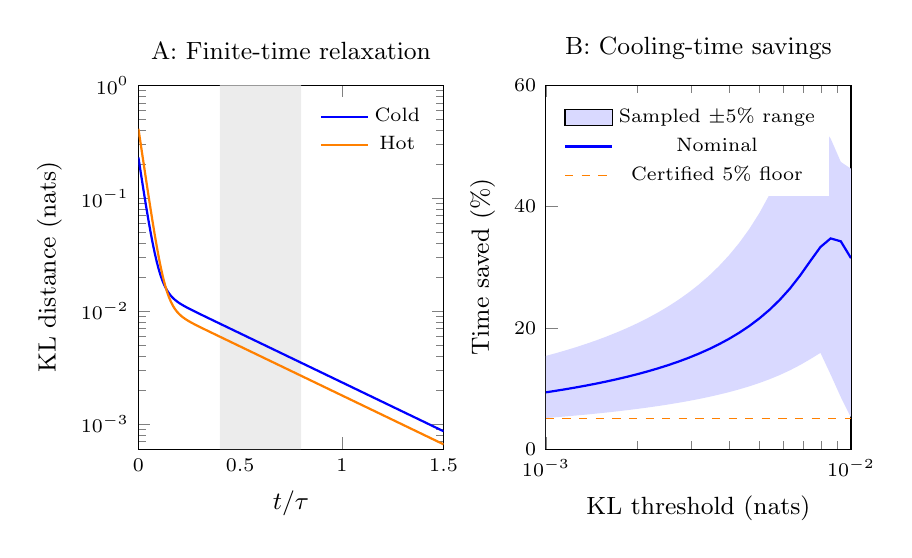
\begin{tikzpicture}
\begin{groupplot}[group style={group size=2 by 1,horizontal sep=1.3cm},
width=0.45\textwidth,height=6.2cm,tick label style={font=\scriptsize},
label style={font=\small},title style={font=\small},
legend style={font=\scriptsize,draw=none}]
\nextgroupplot[title={A: Finite-time relaxation},xlabel={$t/\tau$},
ylabel={KL distance (nats)},ymode=log,xmin=0,xmax=1.5,ymin=0.0006,ymax=1,
legend pos=north east]
\addplot[fill=gray!15,draw=none,forget plot] coordinates {(.4,.0006) (.8,.0006) (.8,1) (.4,1)} \closedcycle;
\addplot[blue,thick] coordinates {(0,0.229831102073) (0.01,0.175461099766) (0.02,0.134421679702) (0.03,0.103493419824) (0.04,0.0802363809521) (0.05,0.062793369371) (0.06,0.0497476452675) (0.07,0.040017862215) (0.08,0.0327793257562) (0.09,0.0274043205061) (0.1,0.0234165111778) (0.11,0.0204558814644) (0.12,0.0182516550588) (0.13,0.0166013223333) (0.14,0.0153543773142) (0.15,0.014399715338) (0.16,0.013655892375) (0.17,0.0130636297951) (0.18,0.0125800828105) (0.19,0.0121744912853) (0.2,0.0118249084438) (0.21,0.0115157635021) (0.22,0.0112360631507) (0.23,0.0109780770569) (0.24,0.0107363858492) (0.25,0.0105071974529) (0.26,0.0102878599123) (0.27,0.0100765166174) (0.28,0.00987186378747) (0.29,0.00967298078028) (0.3,0.0094792118935) (0.31,0.00929008434849) (0.32,0.00910525156273) (0.33,0.00892445401708) (0.34,0.00874749231858) (0.35,0.00857420868916) (0.36,0.00840447426079) (0.37,0.00823818036311) (0.38,0.00807523255162) (0.39,0.00791554651442) (0.4,0.00775904526518) (0.41,0.0076056572162) (0.42,0.0074553148533) (0.43,0.00730795382205) (0.44,0.00716351229536) (0.45,0.00702193053322) (0.46,0.00688315057412) (0.47,0.00674711601643) (0.48,0.00661377186161) (0.49,0.0064830643997) (0.5,0.00635494112405) (0.51,0.00622935066619) (0.52,0.0061062427446) (0.53,0.00598556812322) (0.54,0.00586727857683) (0.55,0.0057513268612) (0.56,0.00563766668676) (0.57,0.00552625269471) (0.58,0.00541704043508) (0.59,0.00530998634614) (0.6,0.00520504773494) (0.61,0.0051021827587) (0.62,0.00500135040694) (0.63,0.0049025104842) (0.64,0.00480562359324) (0.65,0.00471065111882) (0.66,0.00461755521178) (0.67,0.00452629877357) (0.68,0.00443684544113) (0.69,0.0043491595721) (0.7,0.0042632062304) (0.71,0.00417895117207) (0.72,0.00409636083141) (0.73,0.00401540230749) (0.74,0.00393604335083) (0.75,0.00385825235043) (0.76,0.00378199832107) (0.77,0.00370725089081) (0.78,0.0036339802888) (0.79,0.00356215733333) (0.8,0.0034917534201) (0.81,0.00342274051075) (0.82,0.00335509112159) (0.83,0.0032887783126) (0.84,0.00322377567664) (0.85,0.00316005732883) (0.86,0.00309759789623) (0.87,0.00303637250763) (0.88,0.00297635678363) (0.89,0.00291752682686) (0.9,0.00285985921243) (0.91,0.00280333097857) (0.92,0.00274791961741) (0.93,0.00269360306601) (0.94,0.00264035969755) (0.95,0.00258816831264) (0.96,0.0025370081309) (0.97,0.00248685878265) (0.98,0.00243770030073) (0.99,0.00238951311258) (1,0.00234227803241) (1.01,0.00229597625351) (1.02,0.00225058934079) (1.03,0.00220609922339) (1.04,0.0021624881875) (1.05,0.00211973886925) (1.06,0.00207783424783) (1.07,0.00203675763866) (1.08,0.00199649268678) (1.09,0.00195702336029) (1.1,0.00191833394398) (1.11,0.00188040903307) (1.12,0.00184323352705) (1.13,0.00180679262367) (1.14,0.00177107181307) (1.15,0.00173605687194) (1.16,0.00170173385791) (1.17,0.00166808910397) (1.18,0.00163510921303) (1.19,0.00160278105258) (1.2,0.00157109174947) (1.21,0.00154002868478) (1.22,0.00150957948878) (1.23,0.00147973203604) (1.24,0.00145047444056) (1.25,0.00142179505108) (1.26,0.00139368244642) (1.27,0.00136612543092) (1.28,0.00133911303002) (1.29,0.00131263448585) (1.3,0.00128667925301) (1.31,0.0012612369943) (1.32,0.00123629757665) (1.33,0.00121185106709) (1.34,0.00118788772879) (1.35,0.00116439801717) (1.36,0.00114137257613) (1.37,0.00111880223431) (1.38,0.00109667800145) (1.39,0.00107499106481) (1.4,0.00105373278566) (1.41,0.00103289469585) (1.42,0.00101246849446) (1.43,0.000992446044444) (1.44,0.000972819369457) (1.45,0.000953580650644) (1.46,0.000934722223541) (1.47,0.000916236575028) (1.48,0.000898116340338) (1.49,0.00088035430013) (1.5,0.000862943377617)};\addlegendentry{Cold}
\addplot[orange,thick] coordinates {(0,0.413069576939) (0.01,0.312754517084) (0.02,0.237036355156) (0.03,0.179851751991) (0.04,0.136696373478) (0.05,0.104183043175) (0.06,0.0797453422432) (0.07,0.0614299269517) (0.08,0.0477465818986) (0.09,0.0375576405163) (0.1,0.0299951774924) (0.11,0.0243982923554) (0.12,0.0202652055238) (0.13,0.0172164358556) (0.14,0.0149663662959) (0.15,0.0133012217129) (0.16,0.012061990636) (0.17,0.0111311872289) (0.18,0.0104226141239) (0.19,0.00987347950898) (0.2,0.00943836359925) (0.21,0.00908463534815) (0.22,0.00878900091334) (0.23,0.00853492869733) (0.24,0.00831074681951) (0.25,0.0081082508058) (0.26,0.00792169397059) (0.27,0.00774706154653) (0.28,0.00758155288117) (0.29,0.00742321463971) (0.3,0.00727068257854) (0.31,0.0071230007299) (0.32,0.00697949537699) (0.33,0.00683968756319) (0.34,0.00670323255458) (0.35,0.00656987806806) (0.36,0.00643943551365) (0.37,0.00631176023233) (0.38,0.00618673793512) (0.39,0.00606427540721) (0.4,0.00594429414011) (0.41,0.00582672597115) (0.42,0.00571151009711) (0.43,0.00559859102813) (0.44,0.00548791718424) (0.45,0.00537943993106) (0.46,0.00527311291549) (0.47,0.00516889160641) (0.48,0.00506673297531) (0.49,0.00496659527278) (0.5,0.00486843787038) (0.51,0.00477222114741) (0.52,0.00467790640846) (0.53,0.00458545582202) (0.54,0.00449483237378) (0.55,0.00440599982994) (0.56,0.00431892270756) (0.57,0.0042335662498) (0.58,0.00414989640469) (0.59,0.00406787980626) (0.6,0.00398748375763) (0.61,0.00390867621529) (0.62,0.00383142577443) (0.63,0.00375570165508) (0.64,0.0036814736888) (0.65,0.00360871230592) (0.66,0.00353738852318) (0.67,0.00346747393177) (0.68,0.00339894068566) (0.69,0.00333176149024) (0.7,0.00326590959124) (0.71,0.0032013587639) (0.72,0.00313808330237) (0.73,0.00307605800939) (0.74,0.00301525818609) (0.75,0.00295565962212) (0.76,0.00289723858591) (0.77,0.00283997181516) (0.78,0.00278383650751) (0.79,0.0027288103114) (0.8,0.00267487131716) (0.81,0.0026219980482) (0.82,0.00257016945243) (0.83,0.00251936489387) (0.84,0.00246956414437) (0.85,0.00242074737555) (0.86,0.00237289515087) (0.87,0.00232598841787) (0.88,0.00228000850055) (0.89,0.00223493709194) (0.9,0.00219075624677) (0.91,0.00214744837433) (0.92,0.00210499623143) (0.93,0.00206338291555) (0.94,0.00202259185805) (0.95,0.00198260681764) (0.96,0.00194341187382) (0.97,0.00190499142059) (0.98,0.00186733016022) (0.99,0.00183041309712) (1,0.00179422553191) (1.01,0.00175875305554) (1.02,0.00172398154354) (1.03,0.00168989715042) (1.04,0.00165648630411) (1.05,0.00162373570063) (1.06,0.00159163229869) (1.07,0.0015601633146) (1.08,0.0015293162171) (1.09,0.00149907872241) (1.1,0.00146943878933) (1.11,0.00144038461446) (1.12,0.00141190462747) (1.13,0.00138398748652) (1.14,0.00135662207374) (1.15,0.00132979749081) (1.16,0.00130350305461) (1.17,0.00127772829297) (1.18,0.00125246294052) (1.19,0.0012276969346) (1.2,0.00120342041122) (1.21,0.00117962370119) (1.22,0.00115629732626) (1.23,0.0011334319953) (1.24,0.00111101860068) (1.25,0.00108904821458) (1.26,0.00106751208549) (1.27,0.00104640163469) (1.28,0.00102570845286) (1.29,0.00100542429674) (1.3,0.000985541085809) (1.31,0.000966050899137) (1.32,0.000946945972185) (1.33,0.000928218693732) (1.34,0.000909861602851) (1.35,0.000891867385937) (1.36,0.000874228873804) (1.37,0.000856939038826) (1.38,0.000839990992149) (1.39,0.000823377980949) (1.4,0.000807093385747) (1.41,0.000791130717776) (1.42,0.0007754836164) (1.43,0.000760145846589) (1.44,0.000745111296431) (1.45,0.000730373974712) (1.46,0.000715928008525) (1.47,0.000701767640939) (1.48,0.000687887228708) (1.49,0.000674281240029) (1.5,0.000660944252339)};\addlegendentry{Hot}
\nextgroupplot[title={B: Cooling-time savings},xlabel={KL threshold (nats)},
ylabel={Time saved (\%)},xmode=log,xmin=.001,xmax=.01,ymin=0,ymax=60,
legend pos=north west]
\addplot[fill=blue!15,draw=none,area legend] coordinates {(0.001,5.12034706242) (0.00107977516233,5.25298774826) (0.00116591440118,5.39269050865) (0.00125892541179,5.54003489787) (0.00135935639088,5.69566565957) (0.00146779926762,5.86030215575) (0.00158489319246,6.03474948096) (0.00171132830416,6.21991162273) (0.00184784979742,6.41680712254) (0.00199526231497,6.6265878084) (0.00215443469003,6.85056132465) (0.00232630506715,7.09021838652) (0.00251188643151,7.34726595301) (0.00271227257933,7.62366786517) (0.00292864456463,7.92169496726) (0.00316227766017,8.24398735289) (0.00341454887383,8.59363219428) (0.00368694506452,8.97426163302) (0.00398107170553,9.3901763285) (0.00429866234708,9.84650098055) (0.00464158883361,10.3493767645) (0.00501187233627,10.9061868706) (0.00541169526546,11.5257795881) (0.00584341413374,12.2185532679) (0.0063095734448,12.9959703119) (0.00681292069058,13.8682222482) (0.0073564225446,14.8365152472) (0.00794328234724,15.8713220525) (0.00857695898591,12.2877132049) (0.00926118728129,8.56888761073) (0.01,5.18329812309) (0.01,46.2570156307) (0.00926118728129,47.3858708722) (0.00857695898591,51.2323400603) (0.00794328234724,53.4580683359) (0.0073564225446,54.3357430206) (0.00681292069058,53.0193103127) (0.0063095734448,49.5526715625) (0.00584341413374,45.5843851838) (0.00541169526546,42.0288770871) (0.00501187233627,38.9633216503) (0.00464158883361,36.3112679084) (0.00429866234708,33.9967465096) (0.00398107170553,31.9595158307) (0.00368694506452,30.1526198344) (0.00341454887383,28.5391007689) (0.00316227766017,27.0894990624) (0.00292864456463,25.7800480066) (0.00271227257933,24.5913629434) (0.00251188643151,23.5074760881) (0.00232630506715,22.5151155467) (0.00215443469003,21.6031594569) (0.00199526231497,20.7622175822) (0.00184784979742,19.9843069487) (0.00171132830416,19.2625977562) (0.00158489319246,18.5912124228) (0.00146779926762,17.9650652349) (0.00135935639088,17.3797333438) (0.00125892541179,16.8313521857) (0.00116591440118,16.3165300936) (0.00107977516233,15.8322781166) (0.001,15.375951976)} \closedcycle;\addlegendentry{Sampled $\pm5\%$ range}
\addplot[blue,thick] coordinates {(0.001,9.36019343417) (0.00107977516233,9.6193733786) (0.00116591440118,9.89332575988) (0.00125892541179,10.1833506989) (0.00135935639088,10.4909054679) (0.00146779926762,10.8176289717) (0.00158489319246,11.1653709518) (0.00171132830416,11.5362270118) (0.00184784979742,11.9325808654) (0.00199526231497,12.3571556046) (0.00215443469003,12.8130763182) (0.00232630506715,13.3039471057) (0.00251188643151,13.8339464961) (0.00271227257933,14.4079466182) (0.00292864456463,15.0316633085) (0.00316227766017,15.7118469379) (0.00341454887383,16.4565274158) (0.00368694506452,17.2753320938) (0.00398107170553,18.1799028319) (0.00429866234708,19.1844489587) (0.00464158883361,20.3064855692) (0.00501187233627,21.5678126759) (0.00541169526546,22.9957418333) (0.00584341413374,24.6242446847) (0.0063095734448,26.4930595067) (0.00681292069058,28.6355387686) (0.0073564225446,31.0184914733) (0.00794328234724,33.340215479) (0.00857695898591,34.7558697668) (0.00926118728129,34.2743028445) (0.01,31.5054901455)};\addlegendentry{Nominal}
\addplot[orange,dashed] coordinates {(.001,5) (.01,5)};\addlegendentry{Certified $5\%$ floor}
\end{groupplot}
\end{tikzpicture}
\caption{The constrained Arrhenius candidate of Section~\ref{sec:physicalresults}.
The shaded time interval in A has an interval certificate of at least
$10\%$ KL-distance advantage with cold distance above $10^{-3}$ nats.
The distance claim now holds throughout the simultaneous $\pm5\%$ box.
In B, the nominal model has a certified lower bound of $8.12\%$ time savings
throughout the threshold band. The shaded parameter envelope uses 256 corners
and 3,000 sampled interior points at 31 thresholds; it is not a certificate
for the whole parameter box. The dashed $5\%$ floor is separately
certified throughout the full simultaneous $\pm5\%$ box for every
threshold in the band (Section~\ref{sec:physicalboxcertificate}).
The approximate nominal relaxation time is
$\tau=147.232\,\nu_0^{-1}$.}
\label{fig:physicalfinite}
\end{figure}

\subsection{An energy-conserving thermal-collision realization of the same rates}
\label{sec:thermalcollision}
The Arrhenius network also has an exact stochastic bath realization that
does not invoke a large-barrier escape approximation. This clarifies what
can be physically modeled without claiming a particular material or a
continuum potential. The system retains the same four energies, the same
three shared saddle excesses, and the same eight uncertain parameters.

Give each unordered pair $ij$ an independent Poisson contact clock of
rate $\nu_0$. At a contact, draw a fresh reservoir energy
$Y\geq0$ with density $\beta_b e^{-\beta_bY}$. This is a canonical
reservoir with constant density of energy states. If the system is in
endpoint $j$, the contact changes it to $i$ precisely when
\[
 E_j+Y\geq B_{ij}.
\]
After an accepted contact, the outgoing reservoir energy is
$Y'=Y+E_j-E_i$. Otherwise the state and reservoir energy are unchanged.
Contacts on pairs not containing the current state do nothing.
Because $B_{ij}>\max(E_i,E_j)$, accepted moves always have $Y'\geq0$.
They conserve the combined energy exactly.

\paragraph{Rate reduction and detailed balance.}
Integrating out the independent reservoir mark yields
\[
 a_{ij}=\nu_0\Pr(Y\geq B_{ij}-E_j)
       =\nu_0e^{-\beta_b(B_{ij}-E_j)}.
\]
This is the original generator, with its original physical contact clock;
no residence time is deleted and no rate is rescaled to improve the
advantage. For an accepted move the reverse contact is allowed because
$E_i+Y'=E_j+Y\geq B_{ij}$. Applying the map twice returns the original
state and energy, and the translation $Y\mapsto Y'$ preserves its
integration measure. The joint canonical density
$e^{-\beta_b(E_j+Y)}$ is also unchanged. Thus each contact kernel, and
their Poisson superposition, obey detailed balance. These identities
hold throughout the uncertainty box, not just at the nominal point.

Equivalently, with $h_{ij}=B_{ij}-\max(E_i,E_j)$, the rate is
$\nu_0e^{-\beta_bh_{ij}}\min\{1,e^{-\beta_b(E_i-E_j)}\}$.
The acceptance factor is the familiar
\href{https://doi.org/10.1063/1.1699114}{Metropolis form (1953)};
auxiliary-energy simulation methods also have a long history, for example
\href{https://doi.org/10.1103/PhysRevLett.50.1411}{Creutz (1983)}.
No new thermostat or sampling algorithm is claimed here.
The contribution of this construction is an explicit bath interpretation
of the particular constrained rate family and its finite-time clock.

\paragraph{A two-coordinate interpretation of the states.}
Label the ordered states by $(x,y)=(0,0),(1,0),(1,1),(0,1)$ and write
\[
 H(x,y)=\epsilon_x x+\epsilon_y y+Jxy,
\quad
(\epsilon_x,\epsilon_y,J)=(E_2,E_4,E_3-E_2-E_4).
\]
Nominally these coefficients are approximately
$(0.83089,3.67638,-3.56003)\,k_BT_b$.
The two basins fix $x$; their internal degree of freedom is $y$.
Within basin $A$, its excited configuration is expensive, whereas the two
configurations in basin $B$ are nearly degenerate. The exact equilibrium
basin free energies are
\[
 F_A(T)=-T\log(1+e^{-E_4/T}),\qquad
 F_B(T)=E_2-T\log(1+e^{-(E_3-E_2)/T}),
\]
with $k_B=1$ and $E_1=0$. Their different temperature dependence explains
the changing basin populations used in the slow-mode mechanism. This
interpretation does not assume exact lumpability into two basins. Changes
of these Hamiltonian coefficients are correlated by the independently
perturbed gaps; no additional independent uncertainty claim is made.
Contacts may change one or both coordinates. Thus this is not a claim
about standard single-spin-flip dynamics or an identified spin material.

\paragraph{Independent event-clock check and physical limits.}
An executable algebra check verifies the canonical tail integral, energy
conservation and the contact involution. An independent simulation uses
500,000 trajectories per preparation and Poisson contact counts, with no
fixed time step. It samples the thermal reservoir energies explicitly.
For efficiency it thins only the state-independent gate $Y\geq h_{ij}$:
the retained pair clock has rate $\nu_0e^{-\beta_bh_{ij}}$, and the
conditional reservoir energy is $h_{ij}$ plus a fresh exponential energy.
This exact thinning retains the waiting-time cost of rejected contacts.
At five checked physical times, simulated probabilities agree with direct
matrix exponentials within $0.00118$ in every component, passing the
declared six-standard-error diagnostic envelopes. This Monte Carlo check
is supplementary; the collision-to-generator equality is analytic and
the performance certificates do not depend on sampling.
Code and receipts are \path{research/thermal_collision_model.py} and
\path{research/thermal_collision_audit.json}.

The result is an idealized stochastic collision model. Its assumptions
include fresh independent thermal contacts, a constant reservoir density
of states, Poisson contact clocks and instantaneous energy-conserving
updates. It is not a derivation from an autonomous Hamiltonian, an
identified material or a measured bath. The costs of maintaining the
reservoir/contact process and preparing the two initial temperatures are
not included in the post-quench relaxation comparison. For the activated
landscape interpretation, intrawell equilibration and the accuracy of a
continuum escape-rate approximation remain separate physical questions.
The collision realization avoids that approximation within its stated
stochastic assumptions; it does not validate it for a material.

\subsection{An explicit activated-intermediate check of the physical clock}
\label{sec:activatedintermediates}
The four-well study can be extended to retain time spent in transition
regions. This gives a mesoscopic check of one coarse-graining assumption,
not a derivation from a continuum potential or an experimental system.
For each of the six well pairs $ij$, add an intermediate $s_{ij}$ with
energy $B_{ij}$ and phase-space weight $\eta>0$. Well weights are one.
At the bath temperature, in the same dimensionless energy convention,
set
\[
 Q_{s_{ij},j}=2\nu_0 e^{-(B_{ij}-E_j)},\qquad
 Q_{j,s_{ij}}=2\nu_0/\eta,
\]
and use the corresponding pair of rates at endpoint $i$. All other
off-diagonal rates vanish. The diagonal entries conserve probability.
The stationary weights are $g_a e^{-E_a}$, where $g_j=1$ and
$g_{s_{ij}}=\eta$. Each edge obeys detailed balance because its equilibrium
flux in either direction is proportional to $2\nu_0 e^{-B_{ij}}$.

An intermediate has total escape rate $4\nu_0/\eta$ and mean residence
time $\eta/(4\nu_0)$. Partitioning $Q$ into well and intermediate blocks
gives the exact identity
\[
 Q_{ww}-Q_{ws}Q_{ss}^{-1}Q_{sw}=M.
\]
Indeed, each entrance rate is twice the original well-to-well rate,
and the next exit chooses either endpoint with probability $1/2$.
Thus the original generator is the exact trace generator when time in
intermediates is deleted. The following calculation instead evolves the
full ten-state generator in physical time, including those residence
times. Both preparations are full weighted Gibbs distributions
$p_a(T)\propto g_a e^{-E_a/T}$, including the intermediate populations.
Distances are KL divergences from the full ten-state bath distribution.

\paragraph{Numerical results and independent checks.}
For each displayed $\eta$, the nominal parameters are unchanged from
Section~\ref{sec:physicalresults}. The threshold grid contains 41
logarithmically spaced values in $[10^{-3},10^{-2}]$. The perturbation
sample contains all 256 corners of the eight-parameter $\pm5\%$ box
and 500 seeded interior points for each fixed $\eta$.
\begin{center}
\begin{tabular}{rrr}
\toprule
$\eta$ & Nominal minimum time saving & Sampled worst time saving\\
\midrule
$0.025$ & $9.5759\%$ & $5.2719\%$\\
$0.050$ & $9.7883\%$ & $5.4207\%$\\
$0.100$ & $10.2036\%$ & $5.7115\%$\\
\bottomrule
\end{tabular}
\end{center}
All 2,268 parameter samples passed the sampled finite-time benchmarks.
The shortest sampled window with at least a $10\%$ distance advantage
was approximately $1.0889\tau$, with the cold distance at least $10^{-3}$
and times below $5\tau$; here $\tau$ is the full model's slow time.
These are finite grids in parameters, thresholds and time, not certificates
over their continuous ranges or over an interval of $\eta$ values.

At $\eta=0.05$, the cold and hot preparations have respectively about
$1.90\%$ and $4.07\%$ probability in intermediates. Independently
constructed 70-digit direct matrix exponentials agree with the spectral
calculation to within $6.55\times10^{-13}$ in KL distance at five checked
times. Independent numerical root solves give cold/hot arrival times
$210.67249/190.05131$ at threshold $10^{-3}$ and
$40.83628/27.51015$ at $10^{-2}$, in $\nu_0^{-1}$ units.
These correspond to $9.78826\%$ and $32.63307\%$ time savings.
The finite-time benefit therefore survives this explicit extension at
the tested points; it is not an artifact of deleting intermediate
residence times in this model.

\paragraph{Scope and remaining work.}
The original moderate bounds still describe the four well energies and
their effective rates. They do \emph{not} describe every state and rate
of the expanded model: its highest transition-state energy is about
$9.32\,k_BT_b$, and its fast intermediate exits make the full directed
rate ratio exceed the original $10^3$ cap. This extension is a separate
test of the physical approximation, not a replacement candidate claimed
to satisfy the original all-state bounds. The phase-space weight is a
transition-region volume parameter, not an integer degeneracy.
No continuum-potential derivation, material identification or absolute
time calibration has been established.

Both finite-time benchmarks throughout the original four-state $\pm5\%$
uncertainty box are now certified in Section~\ref{sec:physicalboxcertificate}.
Earlier interval methods that could not close that box remain historical
incomplete attempts; their enclosure overestimation was not evidence of
negative probabilities or a failed physical benchmark. The completed
spectral and temperature-reduction proof concerns the four-state model.
It does not turn the ten-state numerical checks into a continuous
robustness theorem. The exact stochastic bath realization of
Section~\ref{sec:thermalcollision} supplies an independent interpretation
of the original rates. A specified material or continuum system would
still require its own rate and preparation-weight validation.

The model and nominal scan are in
\path{research/activated_intermediate_model.py}; the independent audit is
\path{research/check_activated_intermediates.py}. Machine-readable results
are \path{research/activated_intermediate_results.json} and
\path{research/activated_intermediate_audit.json}.

\subsection{Other open mathematical questions}
A separate open mathematical question is finite-time relative-entropy heating order for general contrast-Metzler generators outside the quantified bath neighborhood. Theorems~\ref{thm:contrastchainentropy} and~\ref{thm:nearbatheentropy} now settle, respectively, all heating temperatures for tridiagonal contrast generators and both bath sides within $|\beta-\beta_b|(E_n-E_1)\leq2/\sqrt5$. The general case is still open here. Section~\ref{sec:thermalratioobstruction} proves that the monotone-ratio step of the tridiagonal proof cannot simply be assumed for general admissible dynamics. A completed 1200-second search evaluated 6,740,275,200 sampled derivatives in dimensions 4, 5, 6 and 8 and found none negative; this is search evidence, not a proof. A subsequent 3602-second targeted four-state optimizer made 66,396,528 objective calls and found no negative score. Its best candidate remained positive under an independent 100-digit direct matrix exponential; neither search proves absence. The full four-state amplitude supremum and the location of its possible anomalous interval are now settled. For larger state counts, Theorem~\ref{thm:highdimamplitude} supplies the achievable limit $1-3/n$ under all original tests, whereas the general contrast upper bound remains $1-2/n$. A sharp full-premise bound for $n>4$ remains open between these bounds. Proposition~\ref{prop:highdimboundreduction} reduces a matching upper bound to the slow-mode inequality $w_1+w_2\geq2w_3$. Section~\ref{sec:resettraceobstruction} gives an exact obstruction to one natural proof route: even after subtraction of its minimum reset, a generator satisfying every original triplet inequality can have a three-state trace violating $F_{123}\leq0$. The arithmetic implication itself remains unresolved in higher dimension. These questions exploit the new structure rather than searching again for strong effects that the theorem now excludes.

For external review, the package includes explicit generators, two distinct primary counterexample checks, finite-time certificates, the all-dimension contrast proof and symbolic checks, the finite classifier with polynomial-reference audits, and exact sharpness constructions. The package now also includes the Lean verification described in Section~\ref{sec:lean}. The remaining analytic proofs and executable checks are not thereby formalized. All work belongs to the same project; no external human peer review is claimed.

\section{Explicit slow-mode cofactor polynomials}\label{app:cofactors}
The primary counterexample's exact left eigenvector is $w_i=P_i(r)/P_1(r)$, where $r$ is the simple slow root specified in Theorem~1 and
\begin{align*}
P_1(x)={}&3184000000x^3+1287155436000x^2\\
&+74562002576870x+532366138003157,\\
P_2(x)={}&3184000000x^2+9060415184000x+532366138003157,\\
P_3(x)={}&89152000000x^2+14211422840400x+532366138003157,\\
P_4(x)={}&79281600000x^2+28279185628400x+532366138003157.
\end{align*}

\section{The rational slow-mode companion}\label{app:rational}
The data and strict overlap reversal below are verified in Lean, together with an initial-to-eventual Pearson chi-square relaxation reversal. Section~\ref{sec:lean} states the exact coverage and distinguishes the Lean enclosures from the tighter Python-certified intervals printed here.

Keep the same $q$, $a_{12}$, $a_{13}$, $a_{14}$ and $a_{24}$, but set
\[
a_{23}=\frac{330154675693}{1470375000},\qquad
 a_{34}=\frac{1527327066}{151990625}.
\]
Use detailed balance and conservative diagonals as before. Then
\[
w=\left(1,-\frac{759}{1000},-\frac{48957}{80000},-\frac1{250}\right),
\qquad \lambda_2=-\frac{4966671}{250000}
\]
obey $M^\top w=\lambda_2w$ and $q^\top w=0$ by rational arithmetic. Here $N=27567998009/16000000000$ and $v=\diag(q)w/N$.

The characteristic polynomial factors as
\[
\frac{x(250000x+4966671)R(x)}{632507162050000000000000},
\]
where
\begin{align*}
R(x)={}&2530028648200000000x^2\\
&+1002356769715761942000x+50981800562345565497767.
\end{align*}
One root of $R$ lies in $(-337,-336)$ and the other in $(-60,-59)$, as exact endpoint signs show. The rational eigenvalue is therefore the simple slow mode. The companion certificate checks all original predicates strictly and proves
\begin{align*}
b_2(1/1000)&\in(-0.093755177882,-0.093755177881),\\
b_2(1/100)&\in(-0.093857287853,-0.093857287852).
\end{align*}




\section{Explicit rates for the formal sharpness family}\label{app:formalsharp}
This family is the one used in the focused paper's sharp-supremum proof
and in \path{formal/Mpemba/SharpFamily.lean}. It is distinct from the
uniformly gapped construction in Appendix~\ref{sec:quarterlimit}.
For sufficiently small $\varepsilon>0$, use
\[
q=(1,1-\varepsilon/3,3/5,\varepsilon^2),\qquad
w=(1,-4/5,-1/3-4\varepsilon/9+5\varepsilon^3/3,-\varepsilon).
\]
Set $a_{12}=1$ and define
\begin{align*}
P&=15\varepsilon^4-5\varepsilon^3+69\varepsilon^2-20\varepsilon+68,\\
R&=15\varepsilon^3-4\varepsilon-12,\qquad
S=75\varepsilon^3-20\varepsilon+21,\\
a_{13}&=\frac{150\varepsilon^6+640\varepsilon^5+190\varepsilon^4+
459\varepsilon^3+138\varepsilon^2-252\varepsilon-1224}{RP},\\
a_{14}&=\frac{30\varepsilon^3+125\varepsilon^2-42\varepsilon+240}{3P},\\
a_{23}&=\frac{5(3-\varepsilon)(225\varepsilon^5-185\varepsilon^4+
425\varepsilon^3-113\varepsilon^2-60\varepsilon+204)}{SP},\\
a_{24}&=\frac{5(3-\varepsilon)(9\varepsilon^2-2\varepsilon+16)}{3P},
\qquad a_{34}=\frac{3(9\varepsilon^2-2\varepsilon+16)}{P}.
\end{align*}
Detailed balance determines the upward rates and the diagonals conserve
probability. Rational identities give $q^\top w=0$, $M^\top w=-3w$,
$F_{124}=0$ and $G_{234}=0$. To make the continuity argument precise,
write $(a,b,c,d,e,f)=(a_{12},a_{13},a_{14},a_{23},a_{24},a_{34})$ and
$(t,u,v)=(q_2,q_3,q_4)$, and define the cleared expressions
\begin{align*}
\widehat F_{123}&=bt(2+u)-d(2t+u)-2at(1-t),\\
\widehat F_{134}&=cu(2+v)-f(2u+v)-2bu(1-u),\\
\widehat F_{234}&=eu(2t+v)-ft(2u+v)-2du(t-u).
\end{align*}
These have the same signs as the corresponding original $F$ expressions.
The following thirteen rational functions are continuous and strictly
positive at $\varepsilon=0$:
\[
P,-R,S,b,c,d,e,f,d-bt,-\widehat F_{123},-\widehat F_{134},
-\widehat F_{234},\frac{2(\varepsilon-3)(15\varepsilon^2-5\varepsilon-6)}{9P}.
\]
They remain positive on a nonempty interval of positive $\varepsilon$.
The last expression multiplied by $\varepsilon$ equals $e-ct$, giving
$G_{124}<0$ there. The equality $eu=ft$ and $e-ct>0$ imply $cu<f$,
so $G_{134}<0$ as well. All original triplets therefore fail.
The positive contrast coordinates of $w$ and two connecting positive
off-diagonal contrast entries establish that $-3$ is the simple largest
contrast eigenvalue. The formal proof transfers this to the full
generator; it does not assume a numerical eigensystem or a uniform gap.
Appendix~\ref{sec:lean} gives the formal theorem names and reproduction
instructions. The limits with $\varepsilon=e^{-L^2}$,
$\beta_h=L^{-3}$ and $\beta_c=L^{-1}$ complete the sharpness proof.

\end{document}
